\section{Introduction}
The structure and working methodology of smart parking system based on internet of things is mentioned in this chapter. There are mainly three sections in this chapter. The architecture of this device of the proposed model will be discussed in this section. The analysis of this method will be covered here. This chapter provides the discussion on the framework and inner working principle of this system. Various diagrams and flow charts will also be given here.

\section{Diagram/Overview of Framework}
In our thesis we developed a smart car parking system. In this section the overview of working principle of this system is discussed. This system has two parts-hardware part and software part. Hardware part has three parts-data collecting part, data processing part and data transferring part. IR obstacle sensor is used for sensing the slot status. Each slot has different sensor. Sensors send status signal to arduino for processing. After processing signals arduino can know the total slot status of the parking spot. Each slot has a status LED. IF slot is free the light turns on and if slot is not free light turns off. After processing signals arduino send this data to wifi module to send slot status to server. NodeMCU sends data to firebase realtime database to store data. The parking spot has a main gate which is automated. Each slot has its own automated controlled gate. Those gate are remained off all the time. Only at the time when car enter or exit, the gates open automatically. User use android application to access the system. User has to sign up to this system by submitting his E-wallet phone number and car serial number. User can request for a slot. when requests a pin code is generated and displays on the android screen. The user has to input this pin code into the parking device keyboard. If the pin is matched the main gate and the slot gate opened for a certain amount of time. If car is parked then the time counting started. At the time of unparking only from the android application "Unparked" button is pressed the parked time is calculated and from E-banking wallet the bill is paid. The slot gate and main gate is opened for a certain amount of time for leaving the car. All the data will be generated from device and saved to cloud server. There is an alarming feature in this system. If user does not request system for unpark the car from android application and then if someone wants to steal the car from slot, an early alarm will be given and a notification will be generated from server to android application for notifying the car owner.
\begin{figure}[H]
\centering
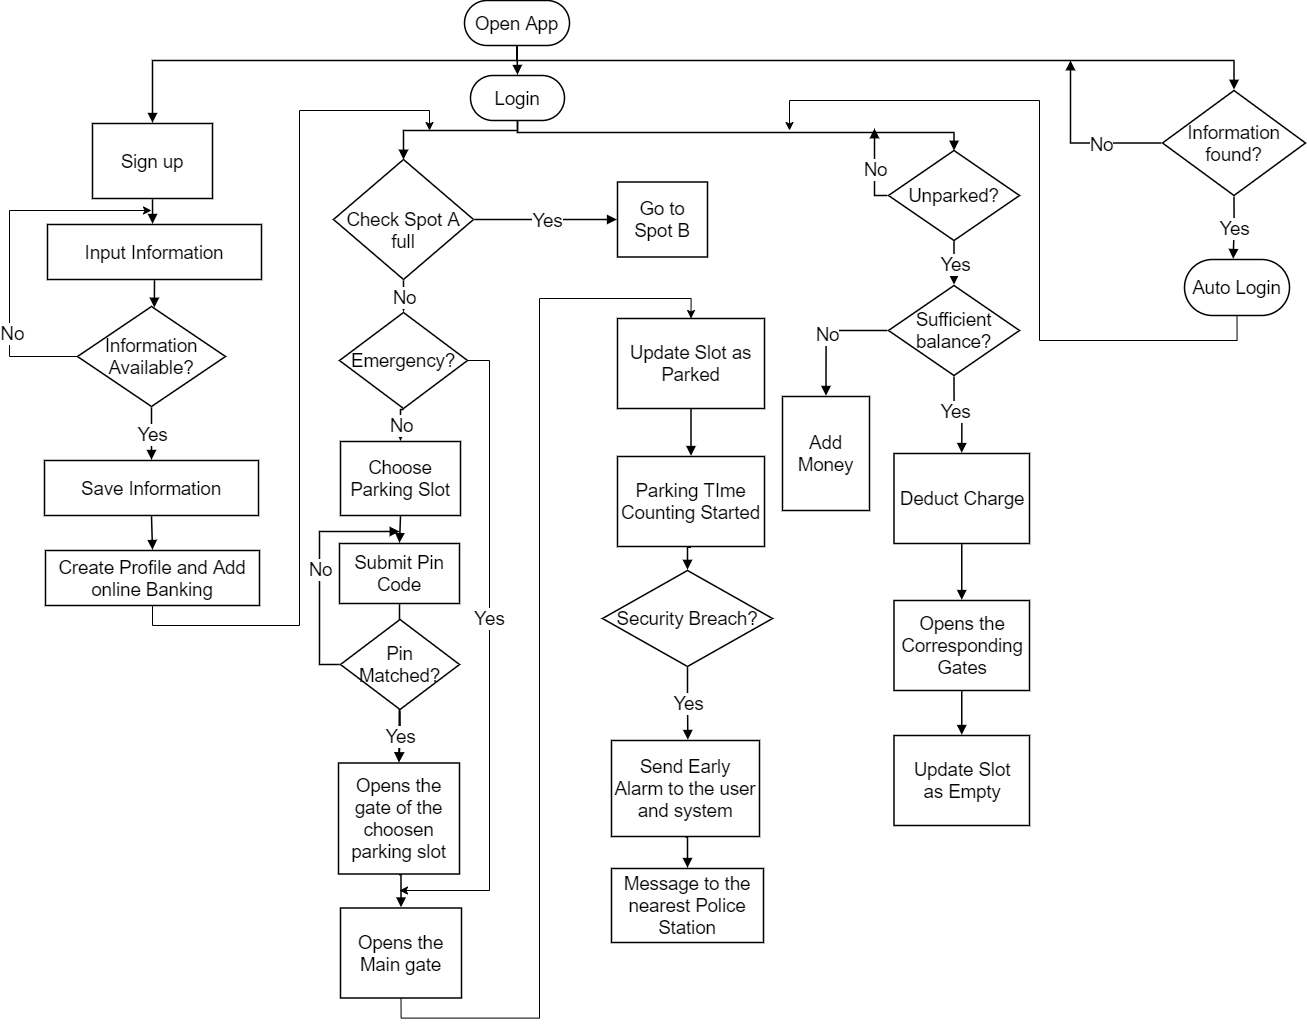
\includegraphics[width=1.0\textwidth]{figures/flowChartFull.png}
\caption{Flow Chart of Developed System}
\label{floww}
\end{figure}
Figure \ref{floww} represents the overall flow chart of our smart parking system.

\section{Feature of This System}
Our system has some features that are given below:
\begin{itemize}
    \item This system can automatically check slot status
    \item This system has LED at each slot for displaying status
    \item This system has automatically controlled gate
    \item This system can update slot status to cloud server
    \item This system has pin verification feature.
    \item This system has anti theft early alarming feature
    \item This system has different advantages for emergency and non emergency parking slot
    \item User can interact with this system using android application
    \item This system has automatically payment feature
    
\end{itemize}{}
\section{Detailed Explanation}
In this system we used different sensor, servo motor, LED, Node MCU, keyboard, Arduino and other hardware. With android application user can use all this feature of this smart parking system. In this section we will discuss on  the circuit diagram, prototype and detailed methodology here.

\begin{figure}[H]
\centering
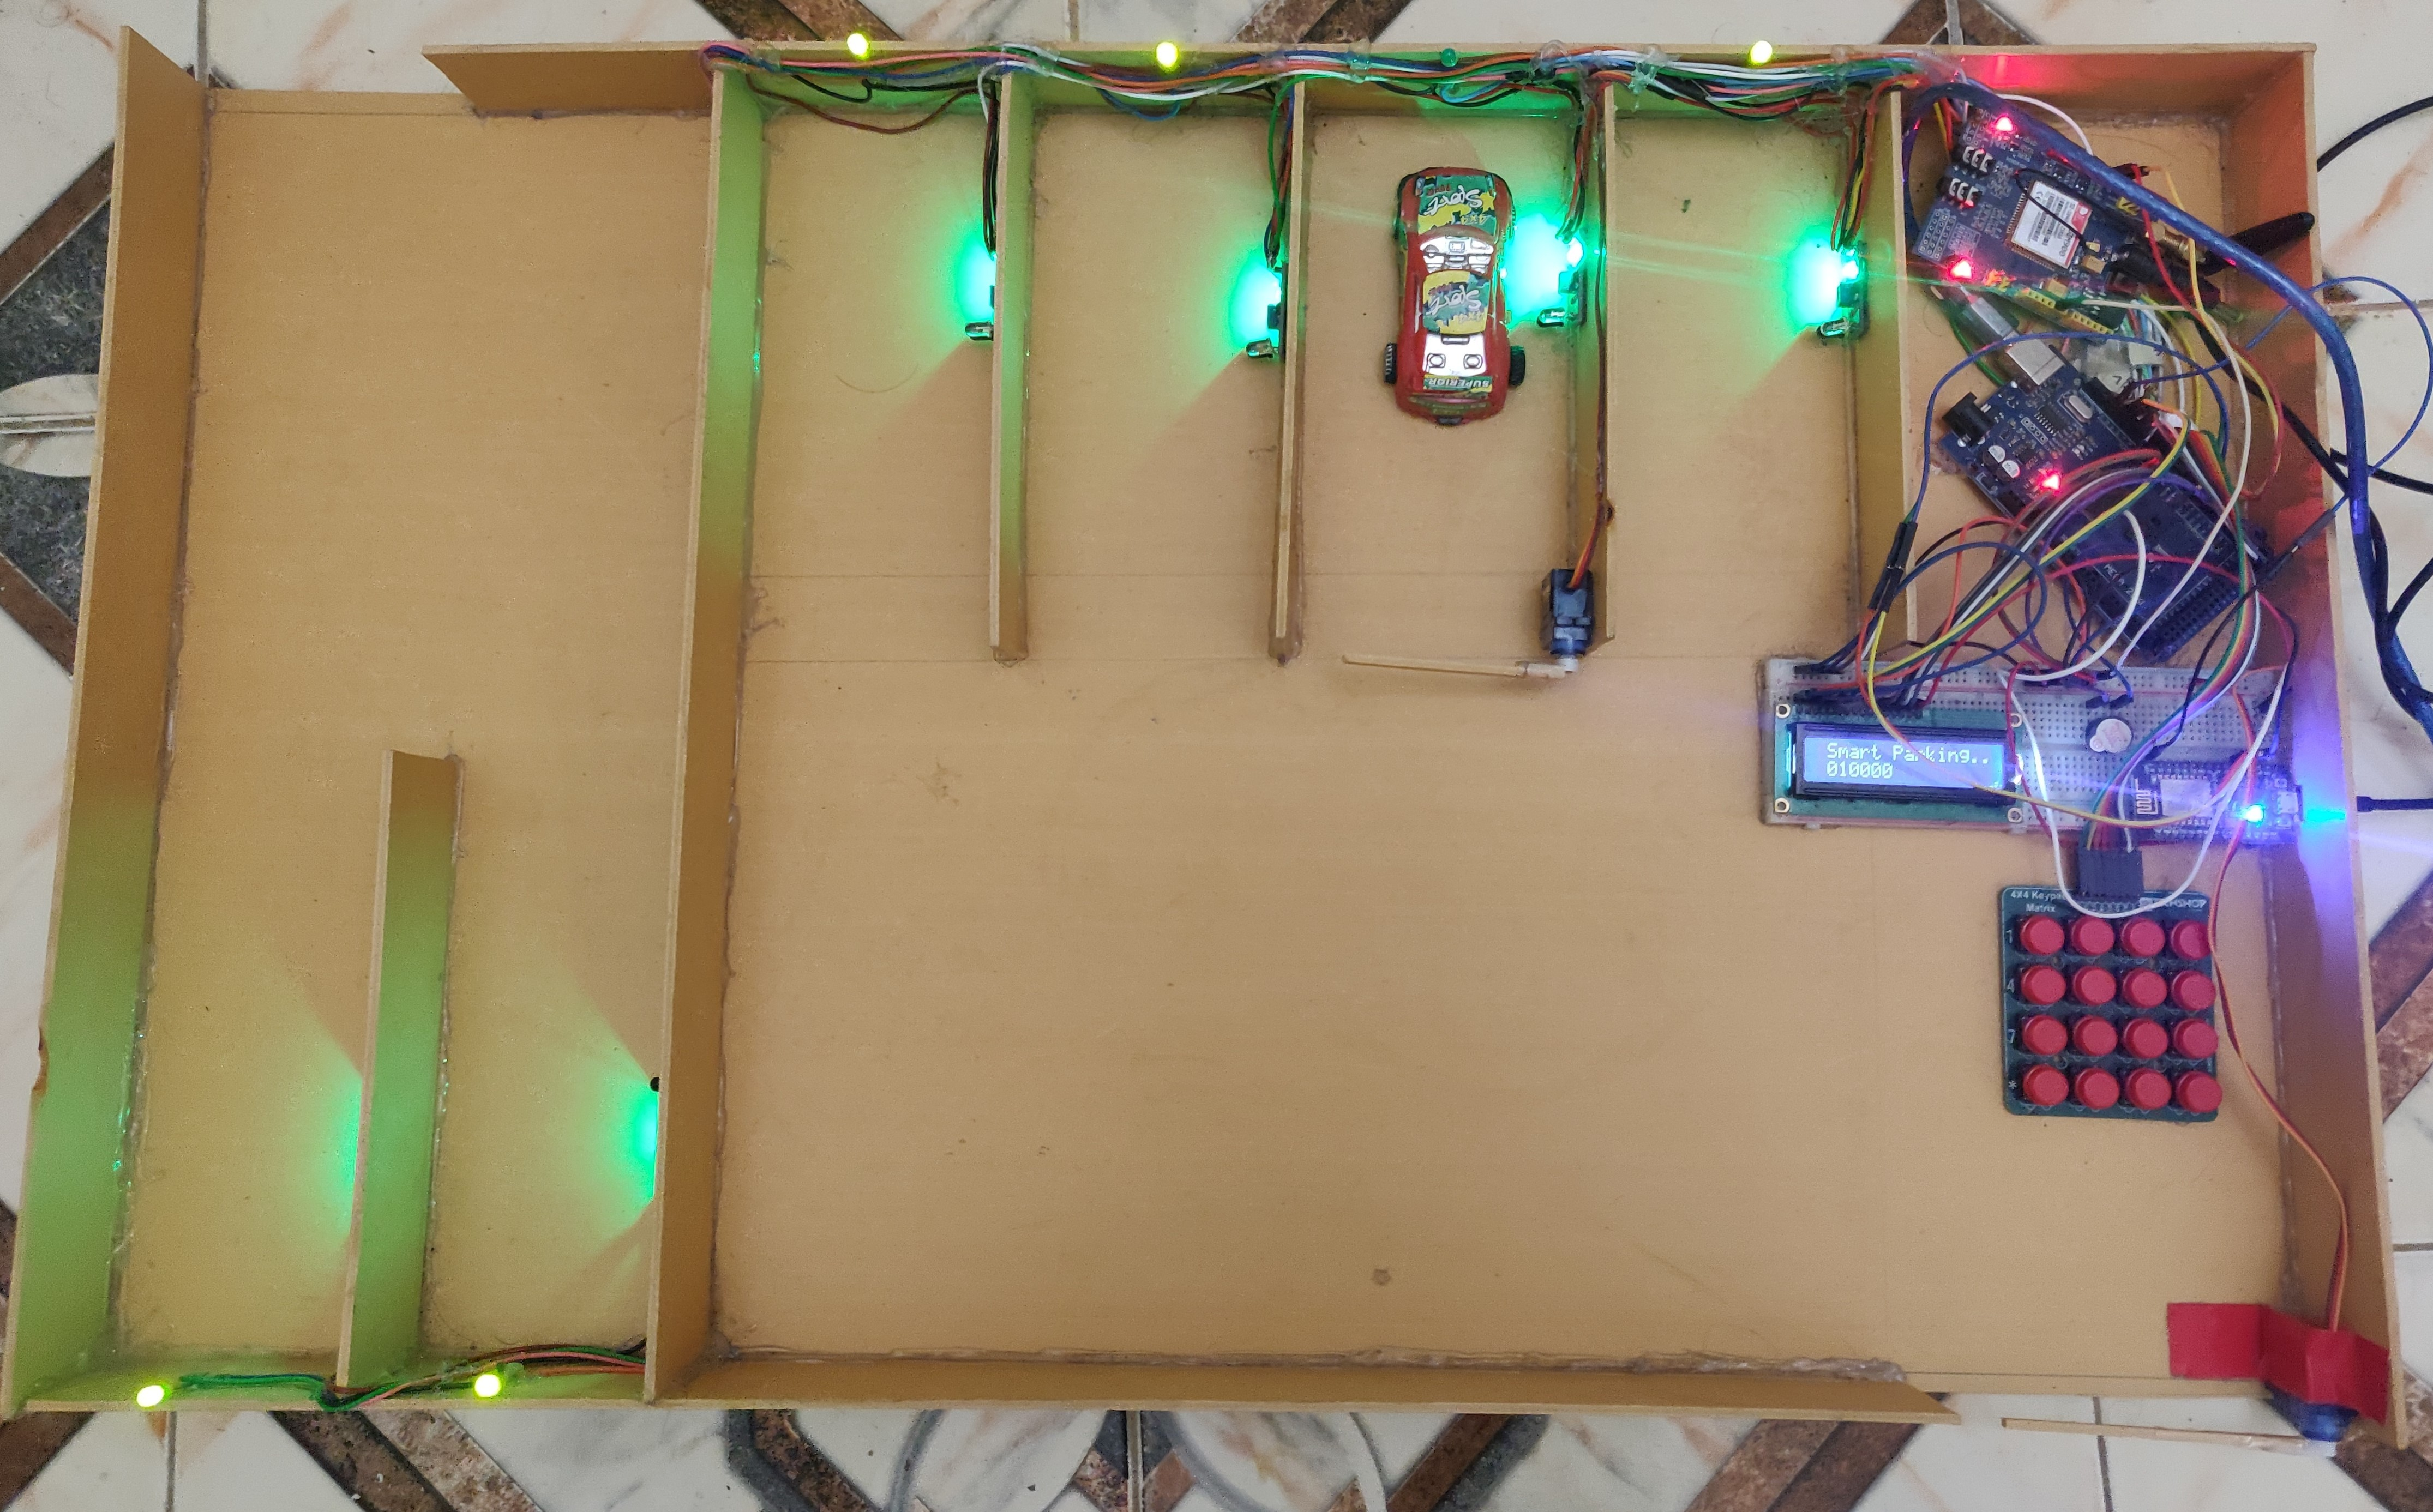
\includegraphics[width=0.5\textwidth]{figures/real_setup.jpg}
\caption{Real Setup of Prototype}
\label{real_setup}
\end{figure}
Figure \ref{real_setup} represents prototype of the real setup of our smart parking system.

\subsection{Schematic Diagram of the System}
The total circuit diagram of this system is given below:

\begin{figure}[H]
\centering
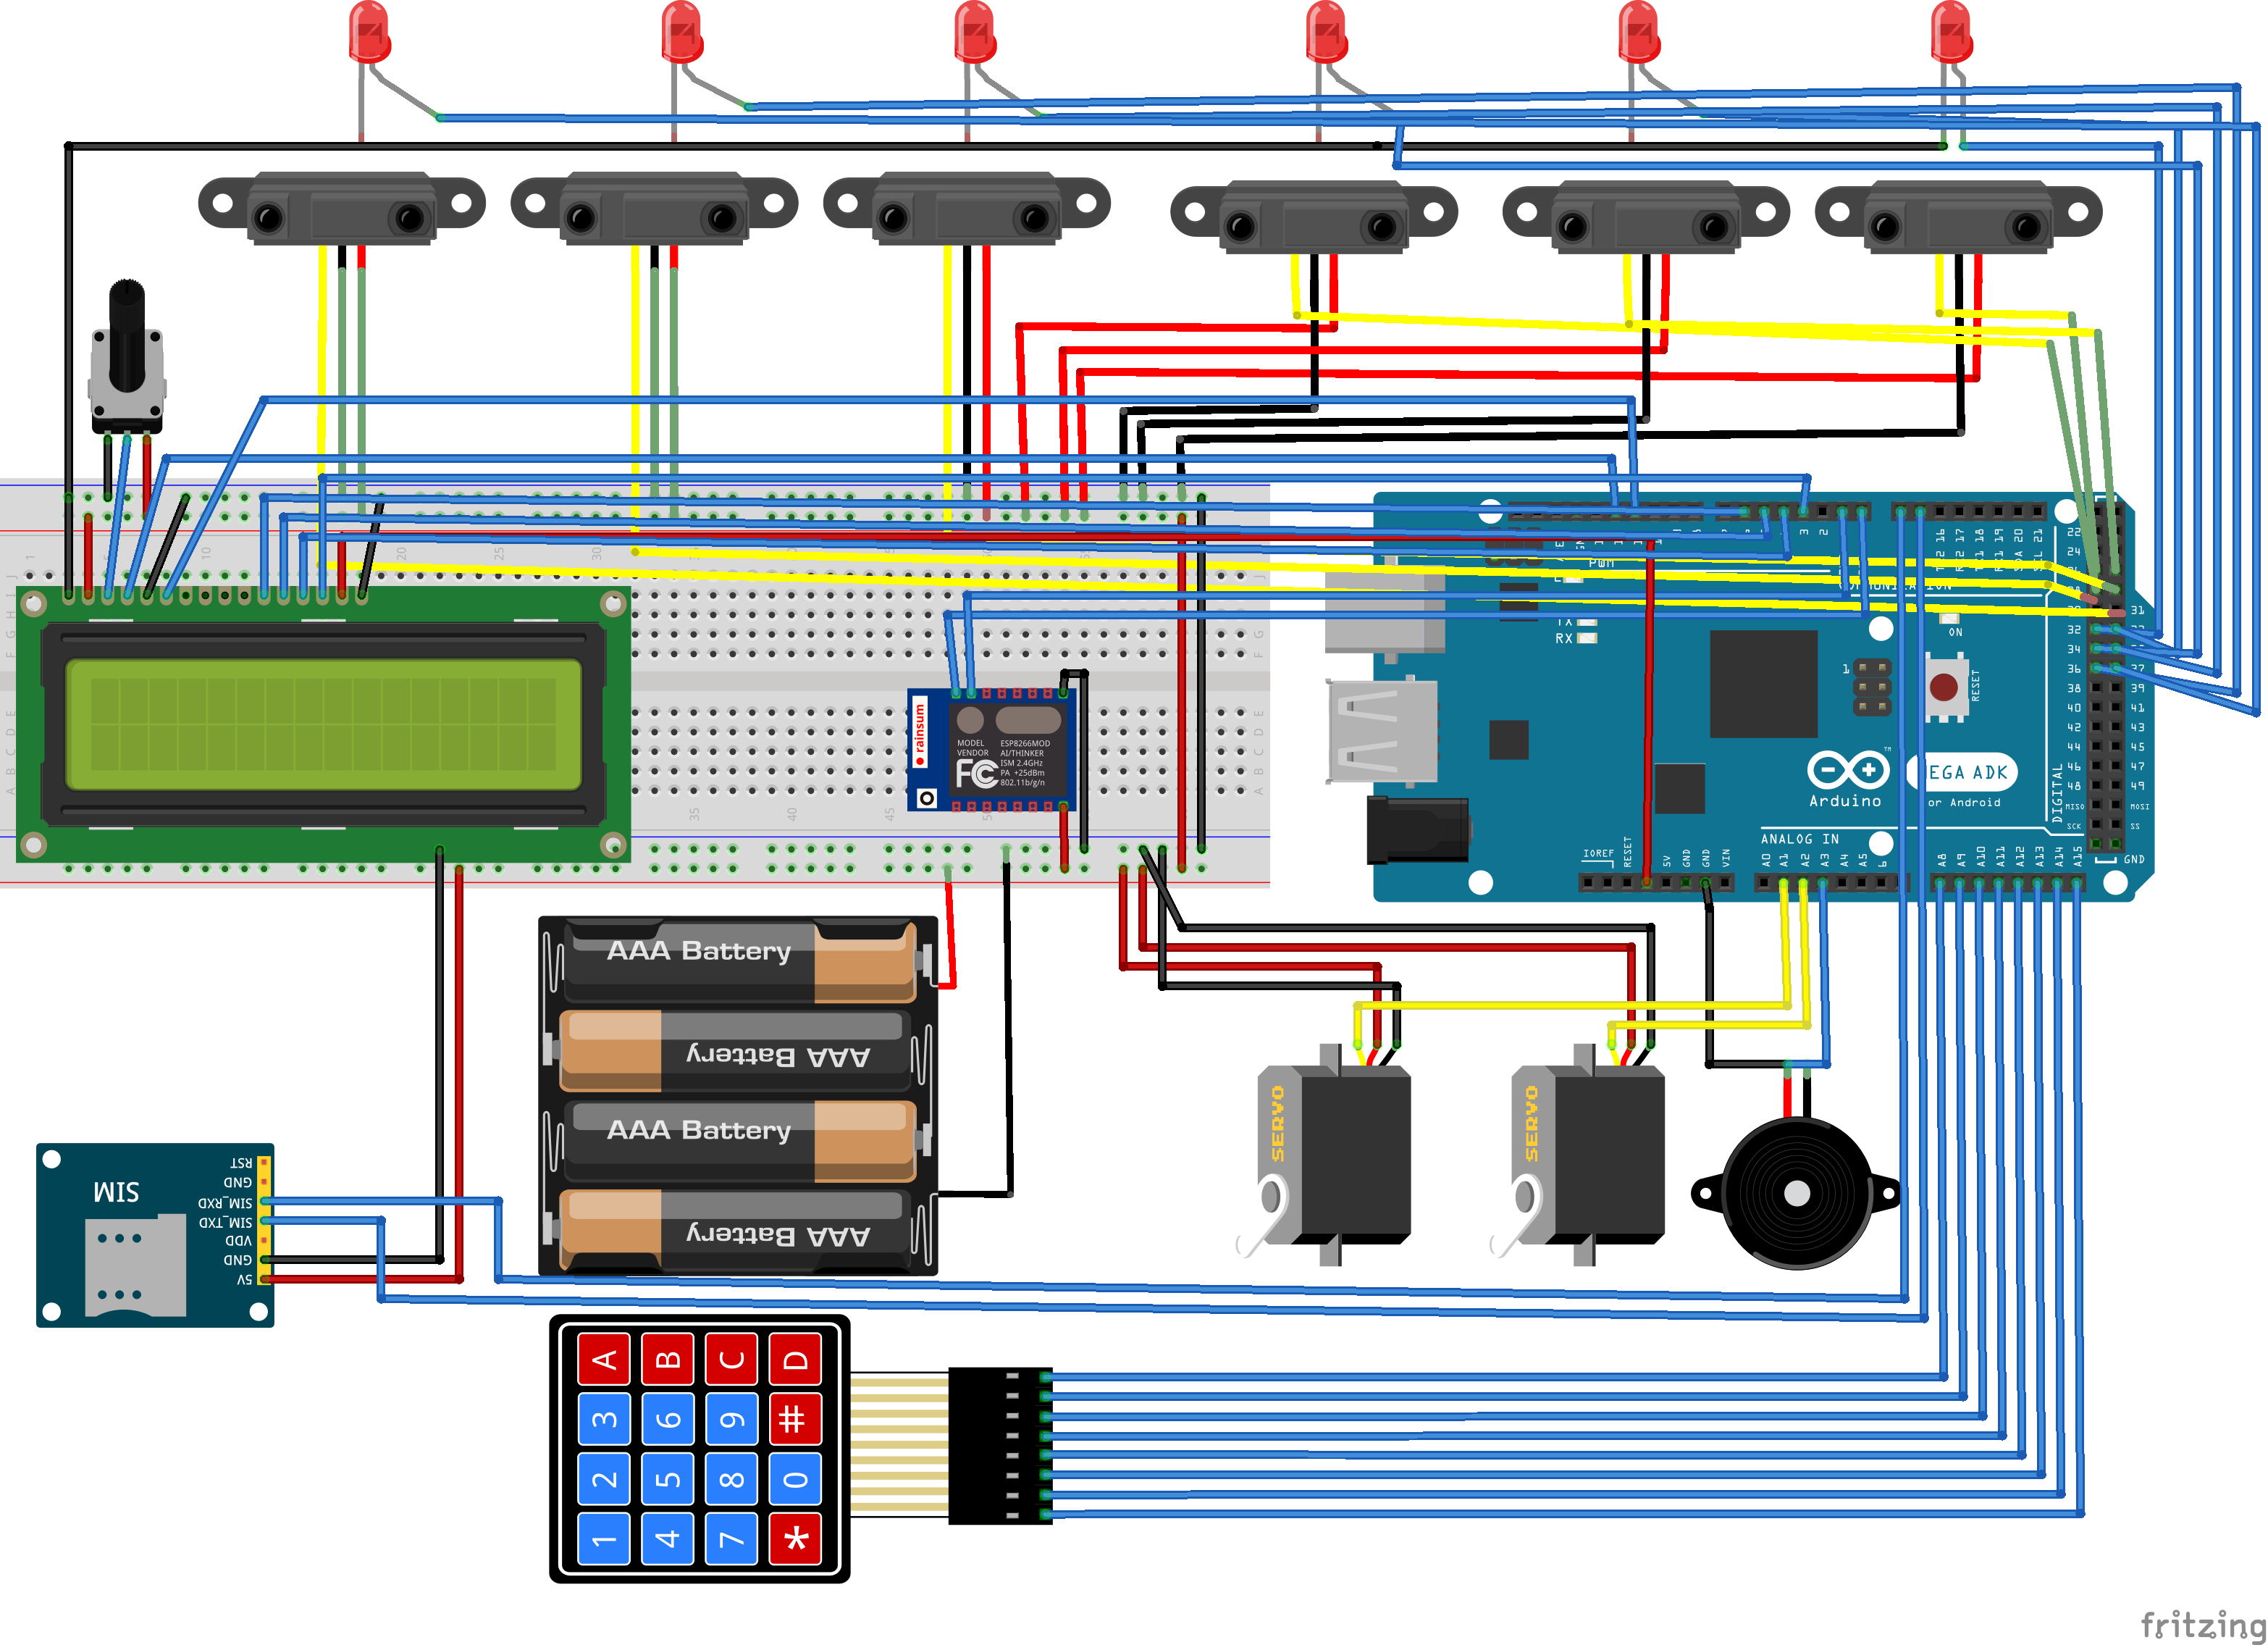
\includegraphics[width=1.0\textwidth]{figures/circuit_diagram.png}
\caption{Circuit Diagram of Smart Parking System}
\label{circuit_diagram}
\end{figure}

Initially all the sensors data is collected by Arduino mega 2560. Each LED is for each slot. In this circuit diagram we can see that each all the component is connected with arduino. It is the controller of this system. After collecting all the sensor data it turn on leds according to slot status and sends slot data to wifi module. Wifi module sends data to server using internet. With android application user can request for a free slot. Here using keypad user can input pin code. Keystroke is taken by arduino. arduino can read this code and check. At the time of parking and unparking gate is opened by servo motor. Buzzer is for making anti theft alarm. When car is placed without requesting for unpark system considers it as  stealing. With wifi module a notification is sent to android application. 
All the data is shown with 16*2 LCD. In the following section we will discuss the working mechanism of each module separately. 

\subsection{Collecting Sensor Data}
For sensing the slot status we used infrared sensor. It has two sensor one is infrared emitter and other is infrared receiver. When there is no car receiver does not receive any signal and it considers as slot is free. When any car parked at the slot the infrared ray is reflected by car and received by IR receiver sensor and it considers as slot is not free.
\begin{figure}[H]
\centering
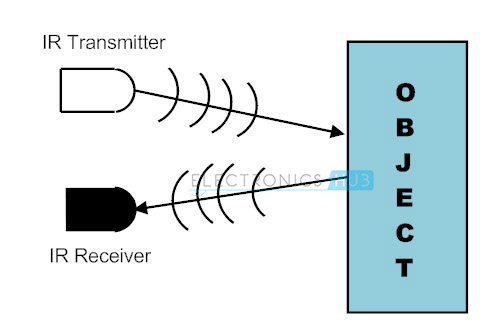
\includegraphics[width=0.5\textwidth]{figures/ir_sensors_work.jpg}
\caption{IR Signal reflections}
\label{ir_work}
\end{figure}

\begin{figure}[H]
\centering
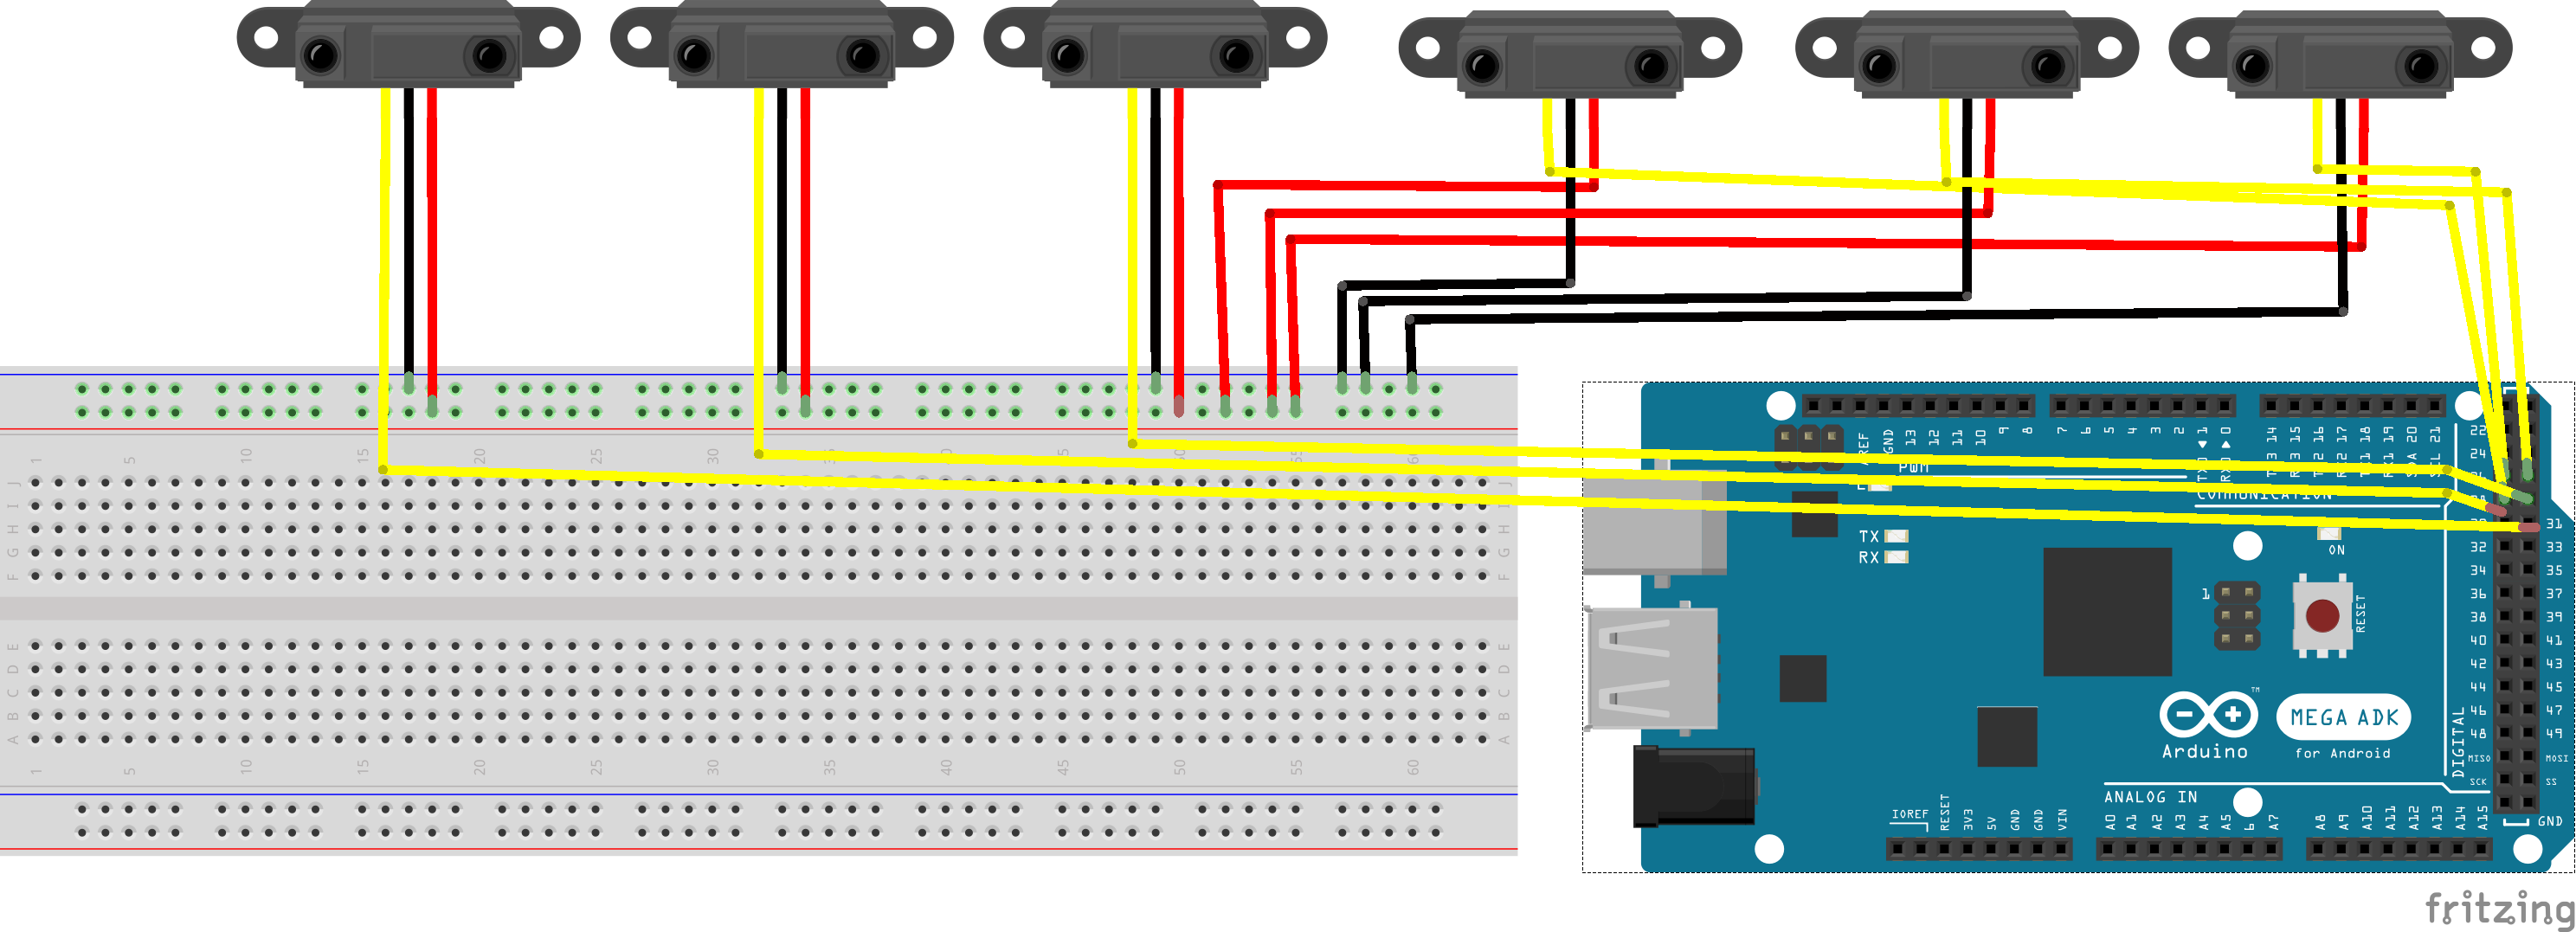
\includegraphics[width=0.8\textwidth]{figures/sensor_bb.png}
\caption{IR Sensor with Arduino}
\label{Ir_sensor_arduino}
\end{figure}
Figure \ref{ir_work} represents the IR sensor working principle. Figure \ref{Ir_sensor_arduino} represents the connection we have used in our system. 

\subsection{LED as status indicator}
Light emitting diode LED is used to indicate the slot status. Each slot has its own LED to indicate its status. If car is parked light is turned off and if the slot is free light is turned on. Figure \ref{light_} shows the connection of LED with arduino. 
% \begin{figure}[H]
% \centering
% 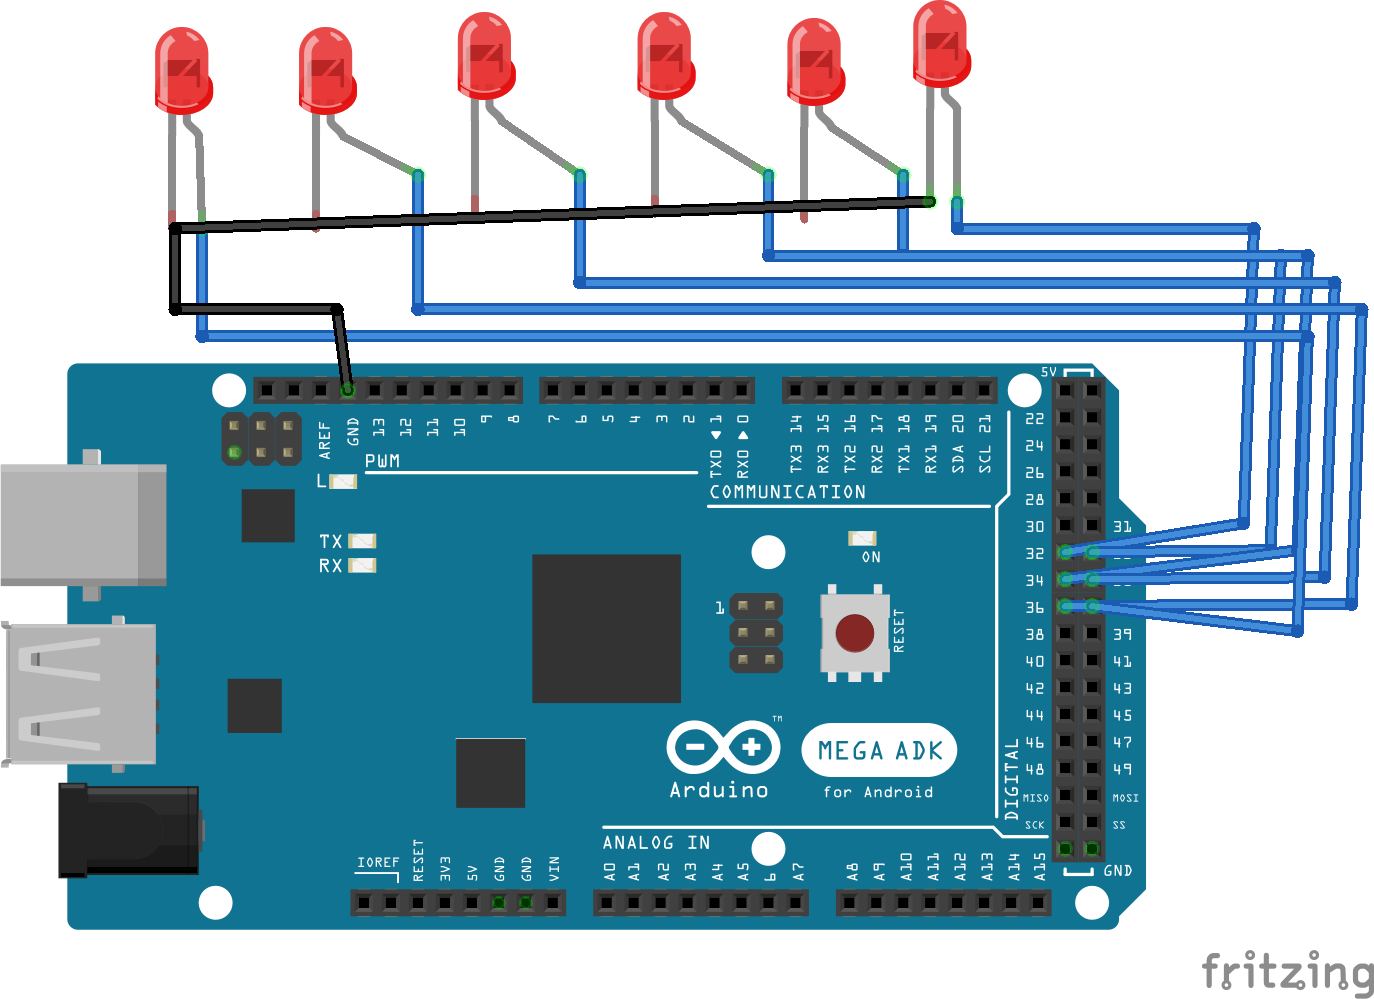
\includegraphics[width=0.5\textwidth]{figures/Led_bb.png}
% \caption{IR Signal reflections}
% \label{light_}
% \end{figure}

% \begin{figure}[H]
% \centering
% 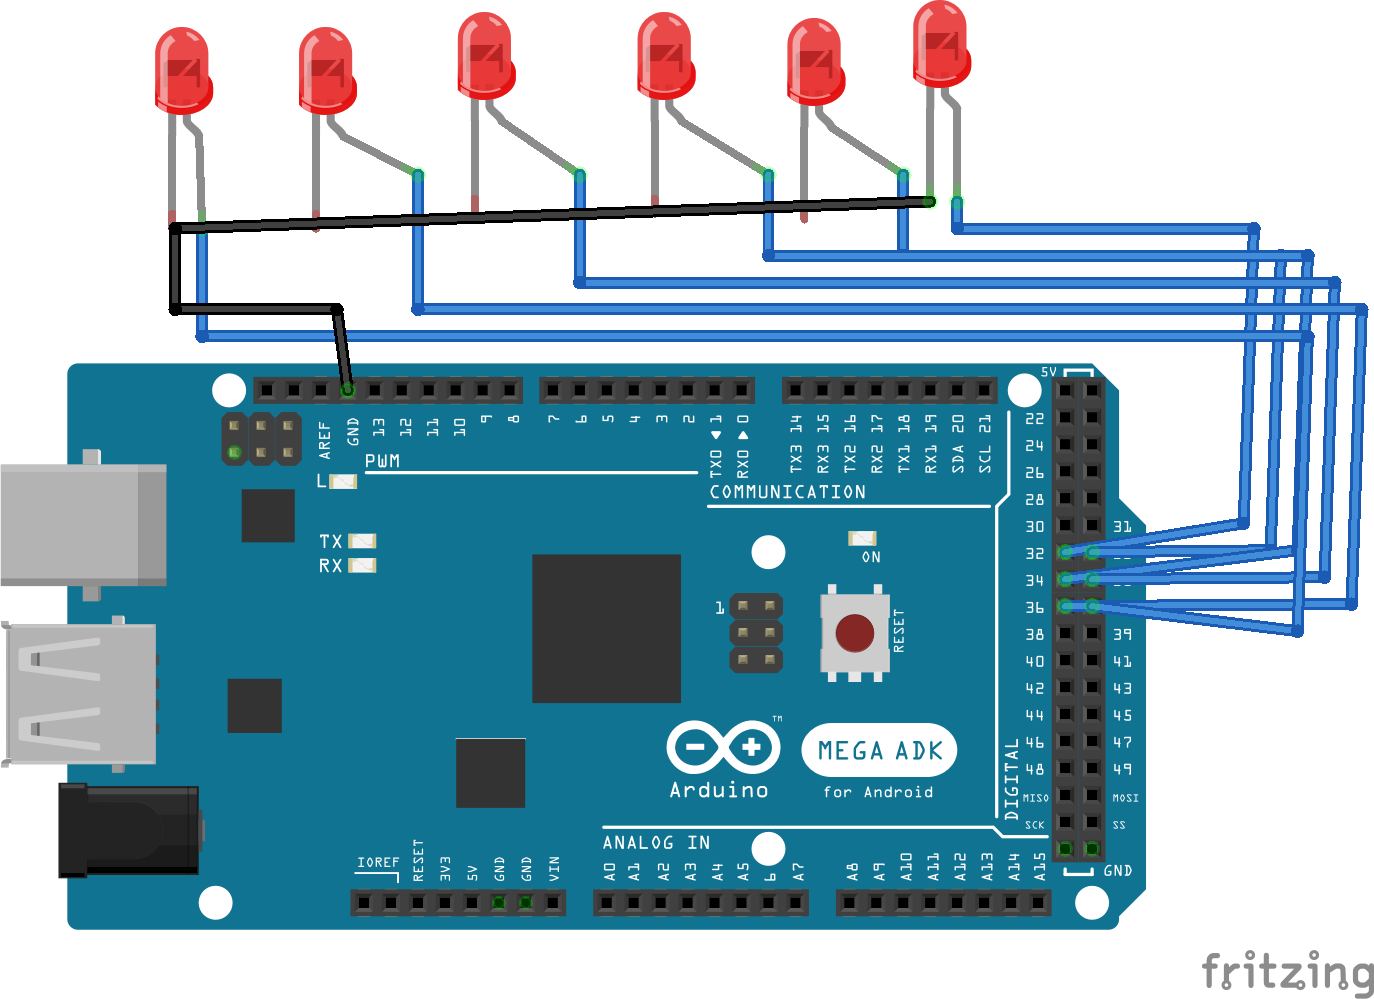
\includegraphics[width=0.5\textwidth]{figures/Led_bb.png}
% \caption{IR Signal reflections}
% \label{ligh_}
% \end{figure}

\begin{figure}[H]
\centering
\subfloat[LED Connected to Arduino]{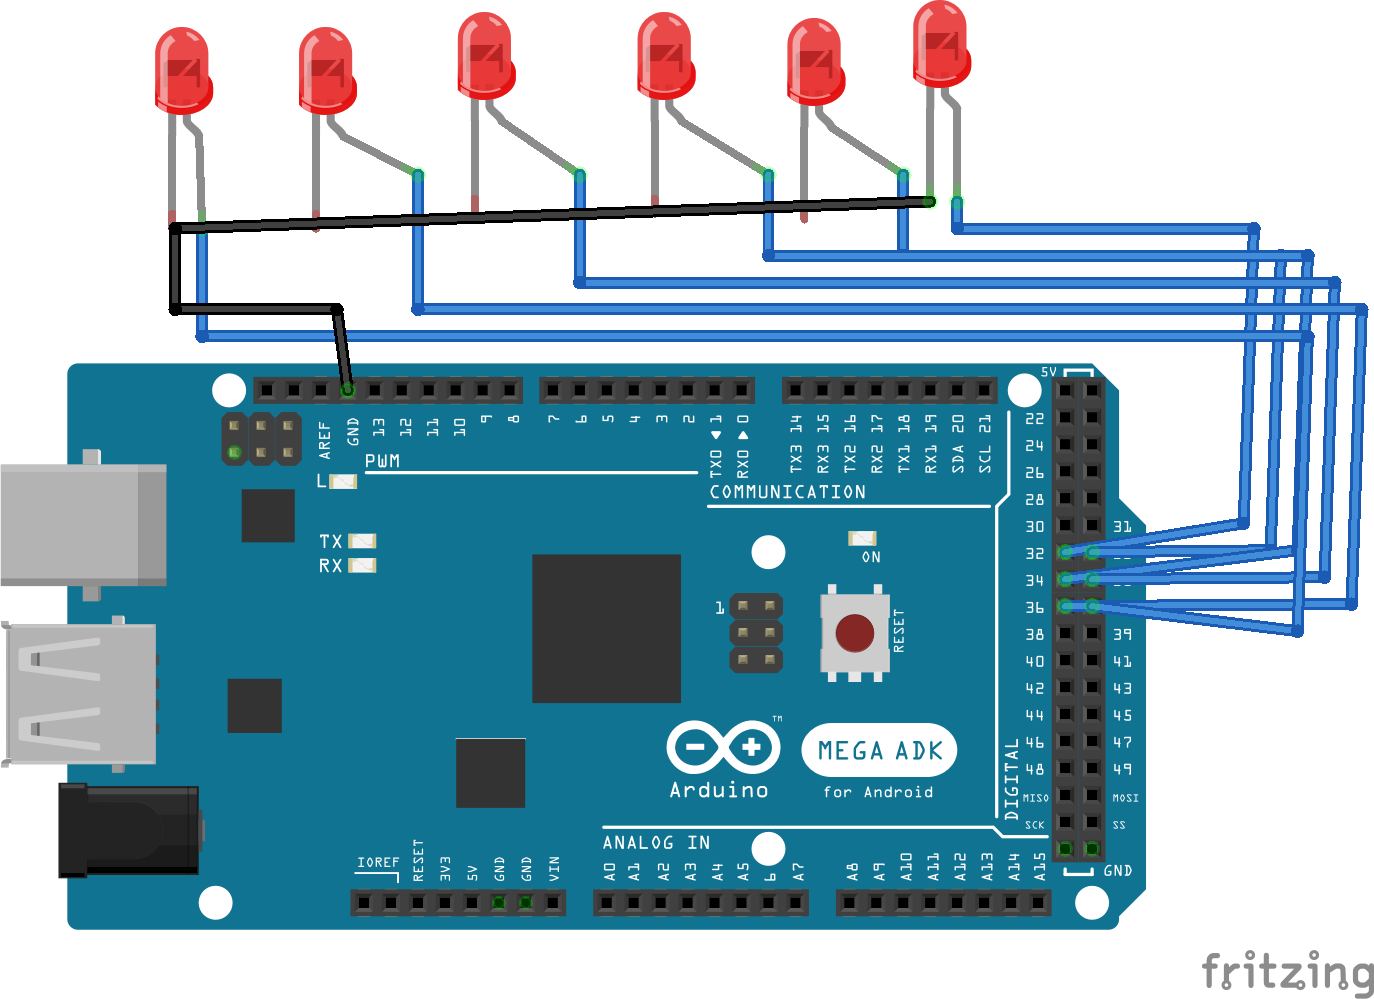
\includegraphics[width = 0.35\textwidth]{figures/Led_bb.png}
\label{light_}} 
\hspace{1cm}
\subfloat[LED at Prototype]{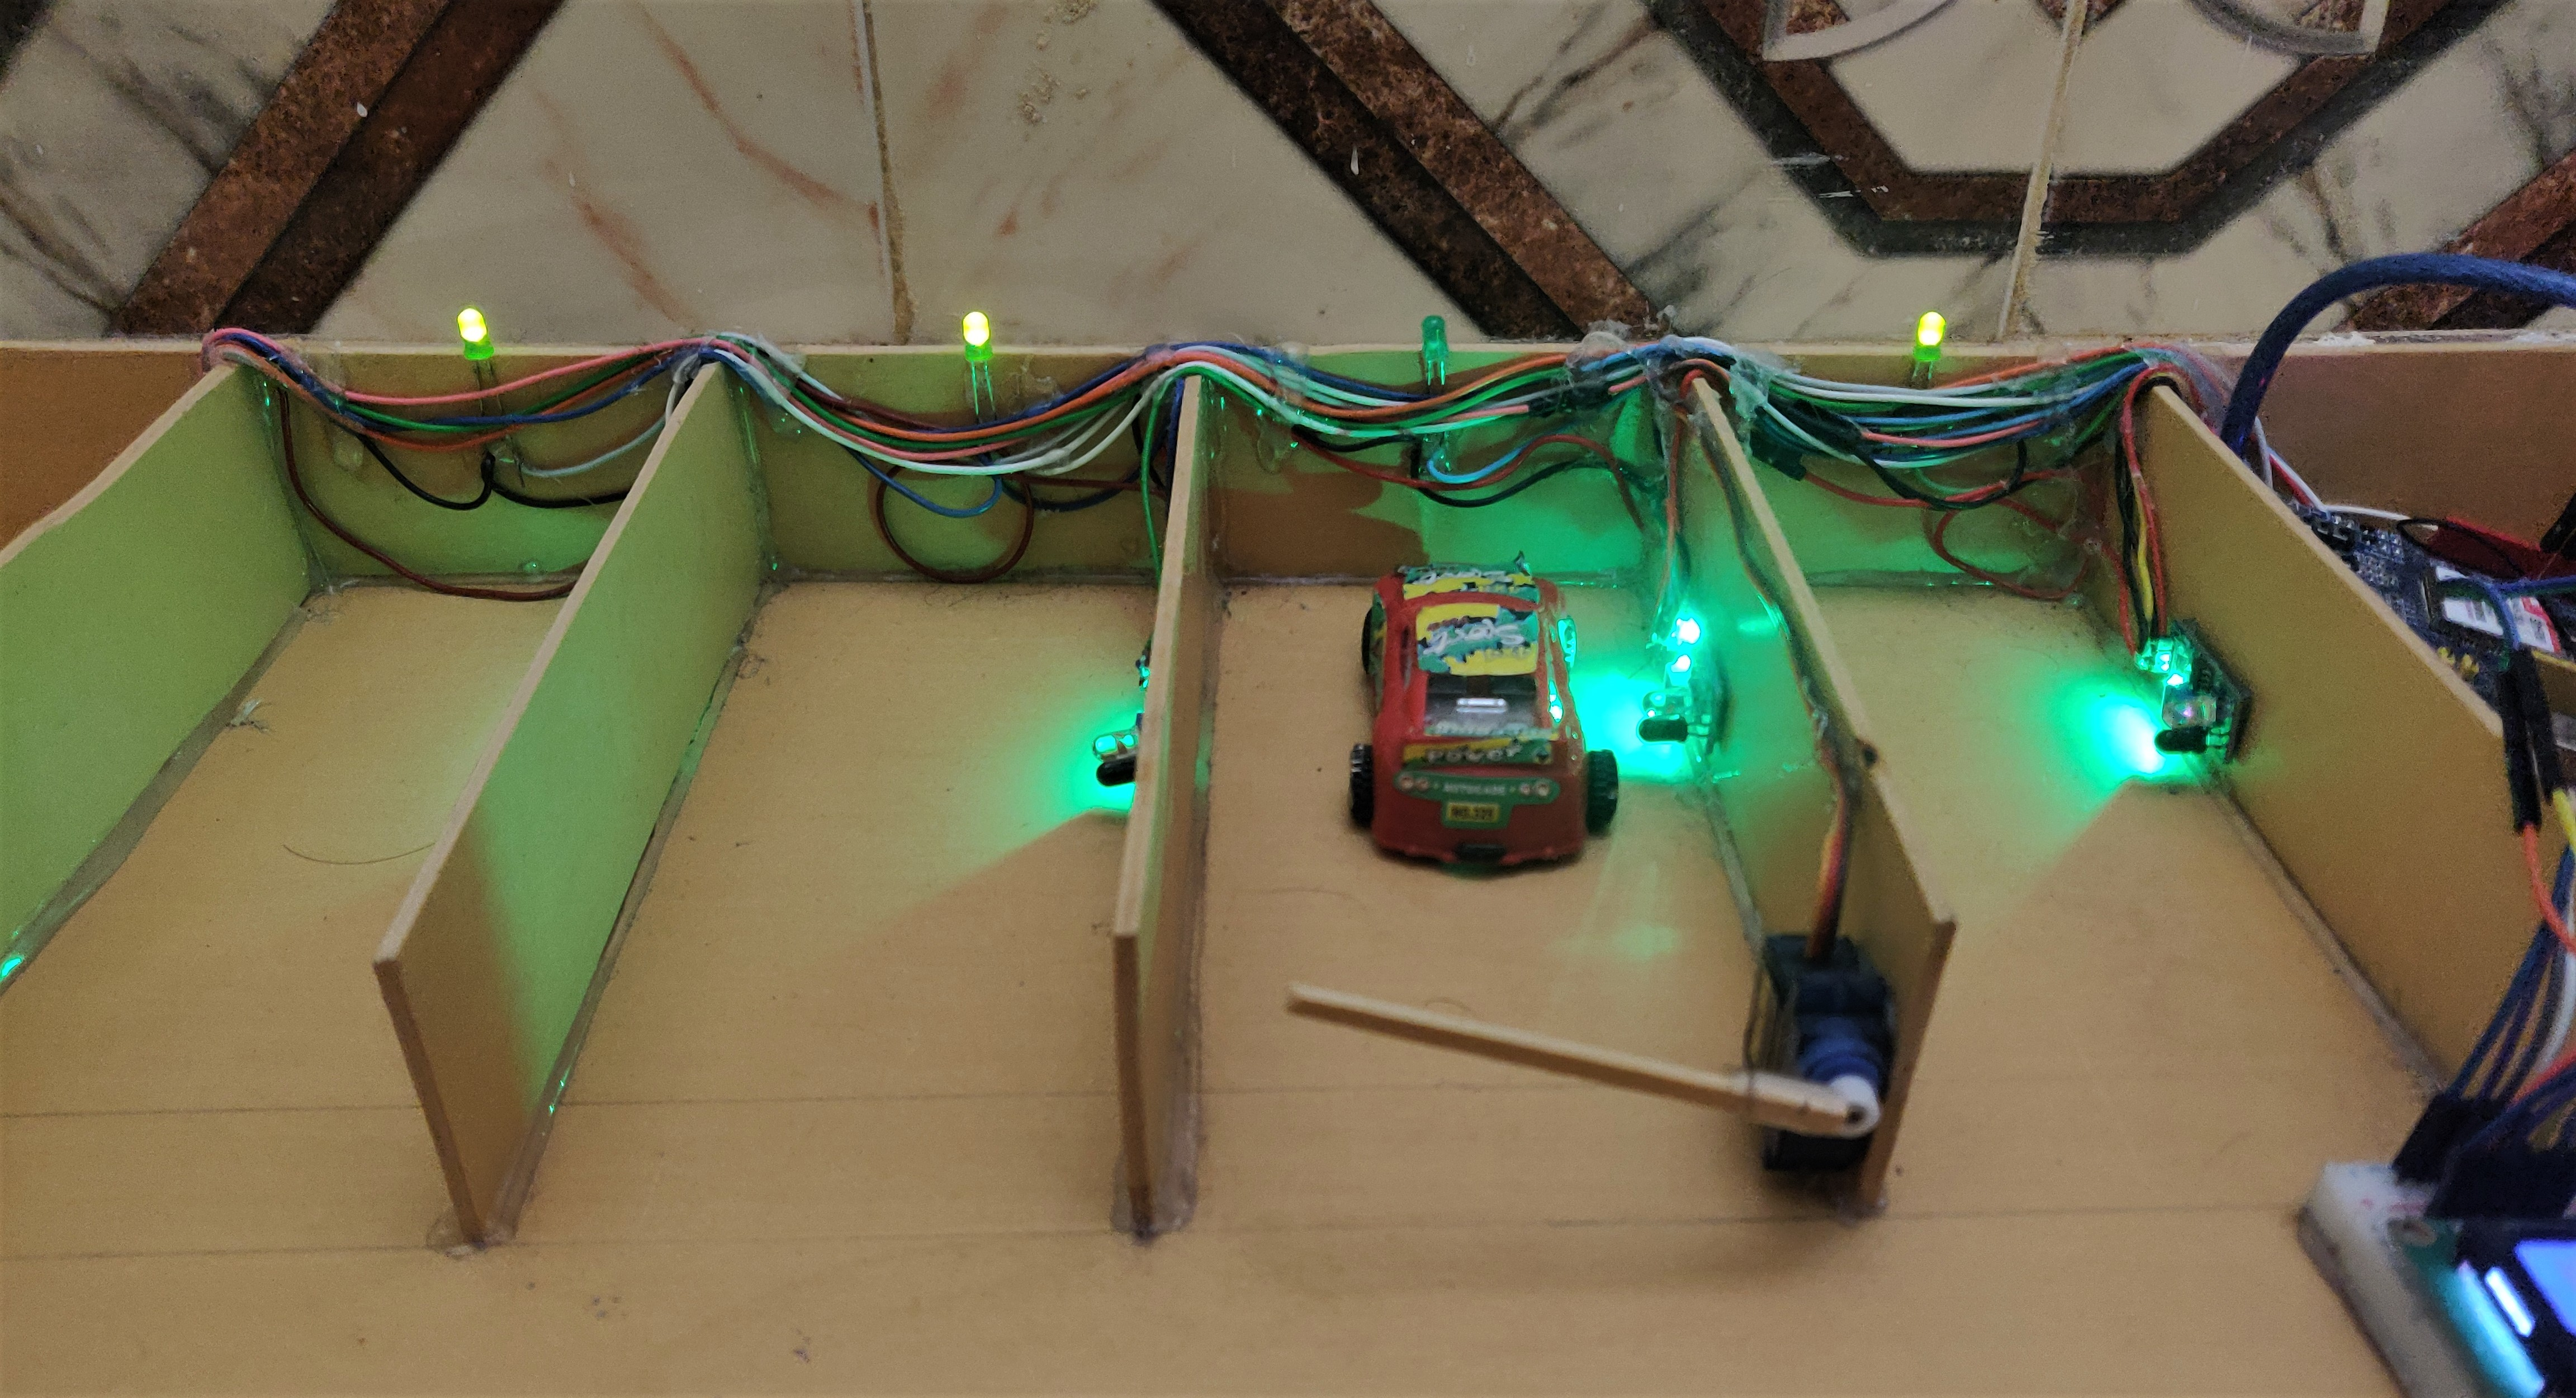
\includegraphics[width = 0.35\textwidth]{figures/slot_led.jpg}
\label{ligh_}}
\caption{LED Indicating Status}
\end{figure}
In figure \ref{ligh_} off LED represents that  slot is not free and other slots are free.

\subsection{Transferring Data to Wifi Module}
After collecting data from sensors arduino transfer data to NodeMCU. Arduino can be conneted to wifi module via universal asynchronous receiver transmitter(UART). In this connection one device Rx is connected to another device Tx and Tx is connected to Rx.
\begin{figure}[H]
\centering
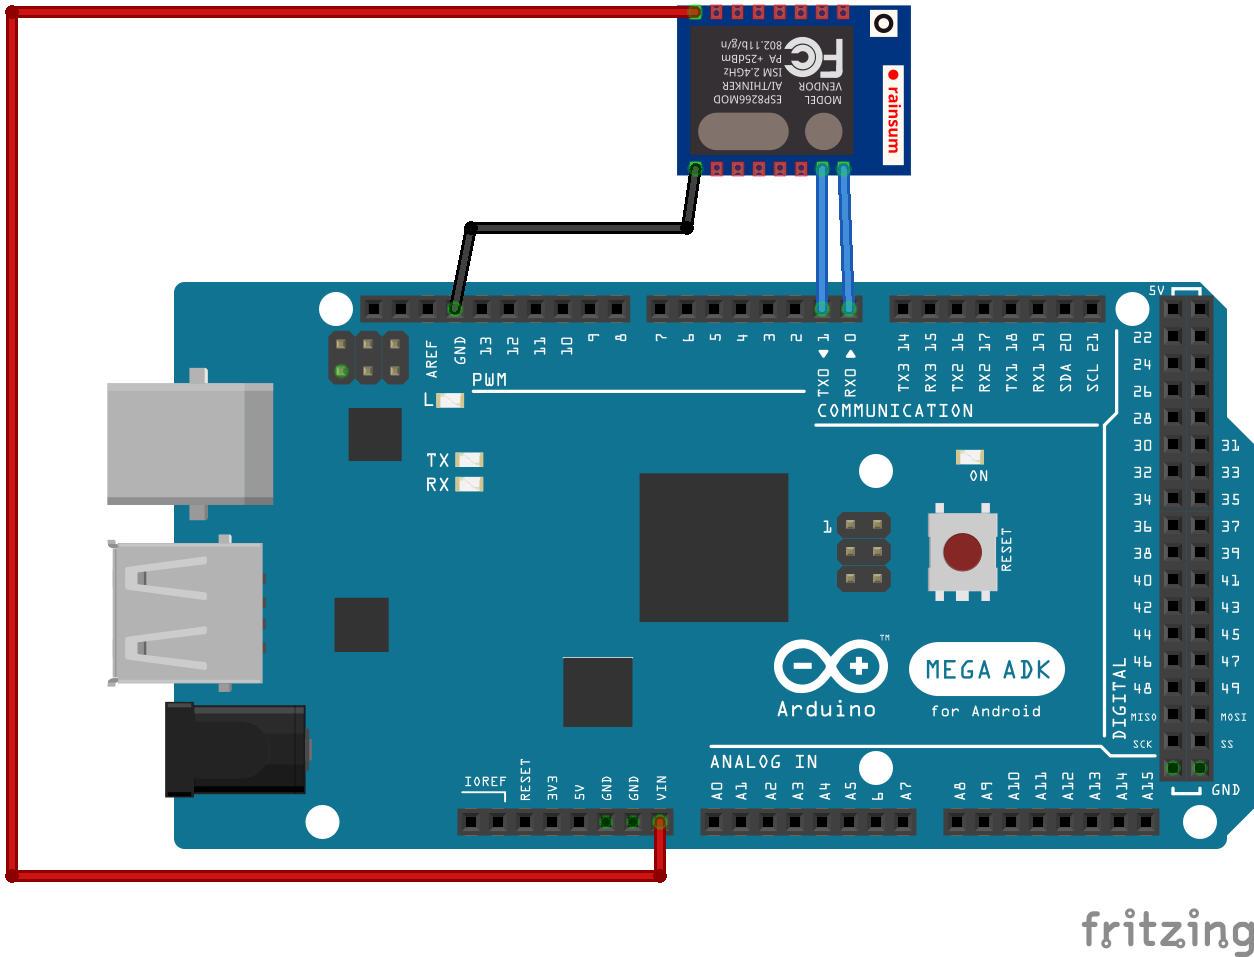
\includegraphics[width=0.5\textwidth]{figures/wifi_bb.png}
\caption{NodeMCU Connection to Arduino}
\label{node1}
\end{figure}
Figure \ref{node2} represents that data is updating to firebase database.

\subsection{Sending Data to Server With Internet}
Wifi module can be connected to local hotspot or any 2.4GHz internet providing network. With Internet It sends data to firebase realtime cloud server to store data. Figure \ref{node1} represents the connection of NodeMCU to arduino.
\begin{figure}[H]
\centering
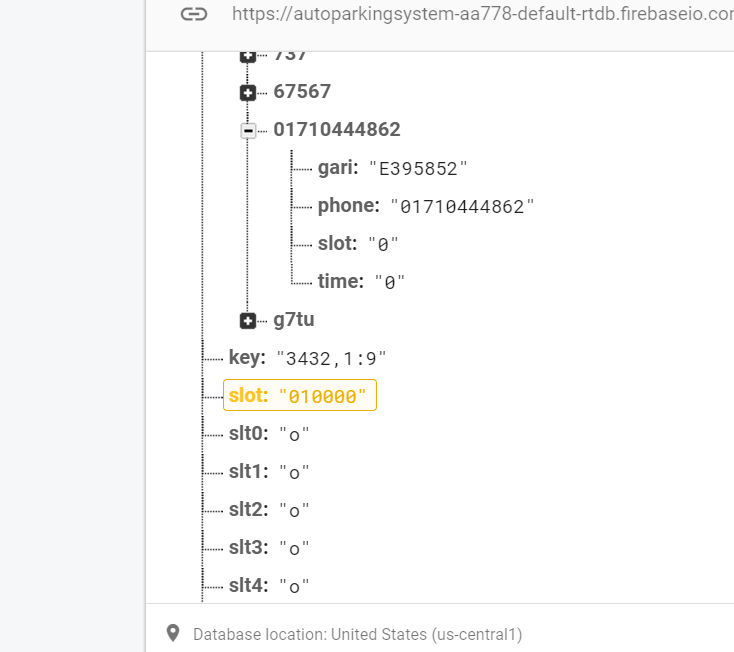
\includegraphics[width=0.5\textwidth]{figures/slot_updating.png}
\caption{Data Updating to Firebase}
\label{node2}
\end{figure}
Figure \ref{node2} represents that data is updating to firebase database.

\subsection{Inputting Pin Code}
For submitting pin code we used 4*4 matrix keyboard. Where 4 pin for row and 4 pin for column. 
\begin{figure}[H]
\centering
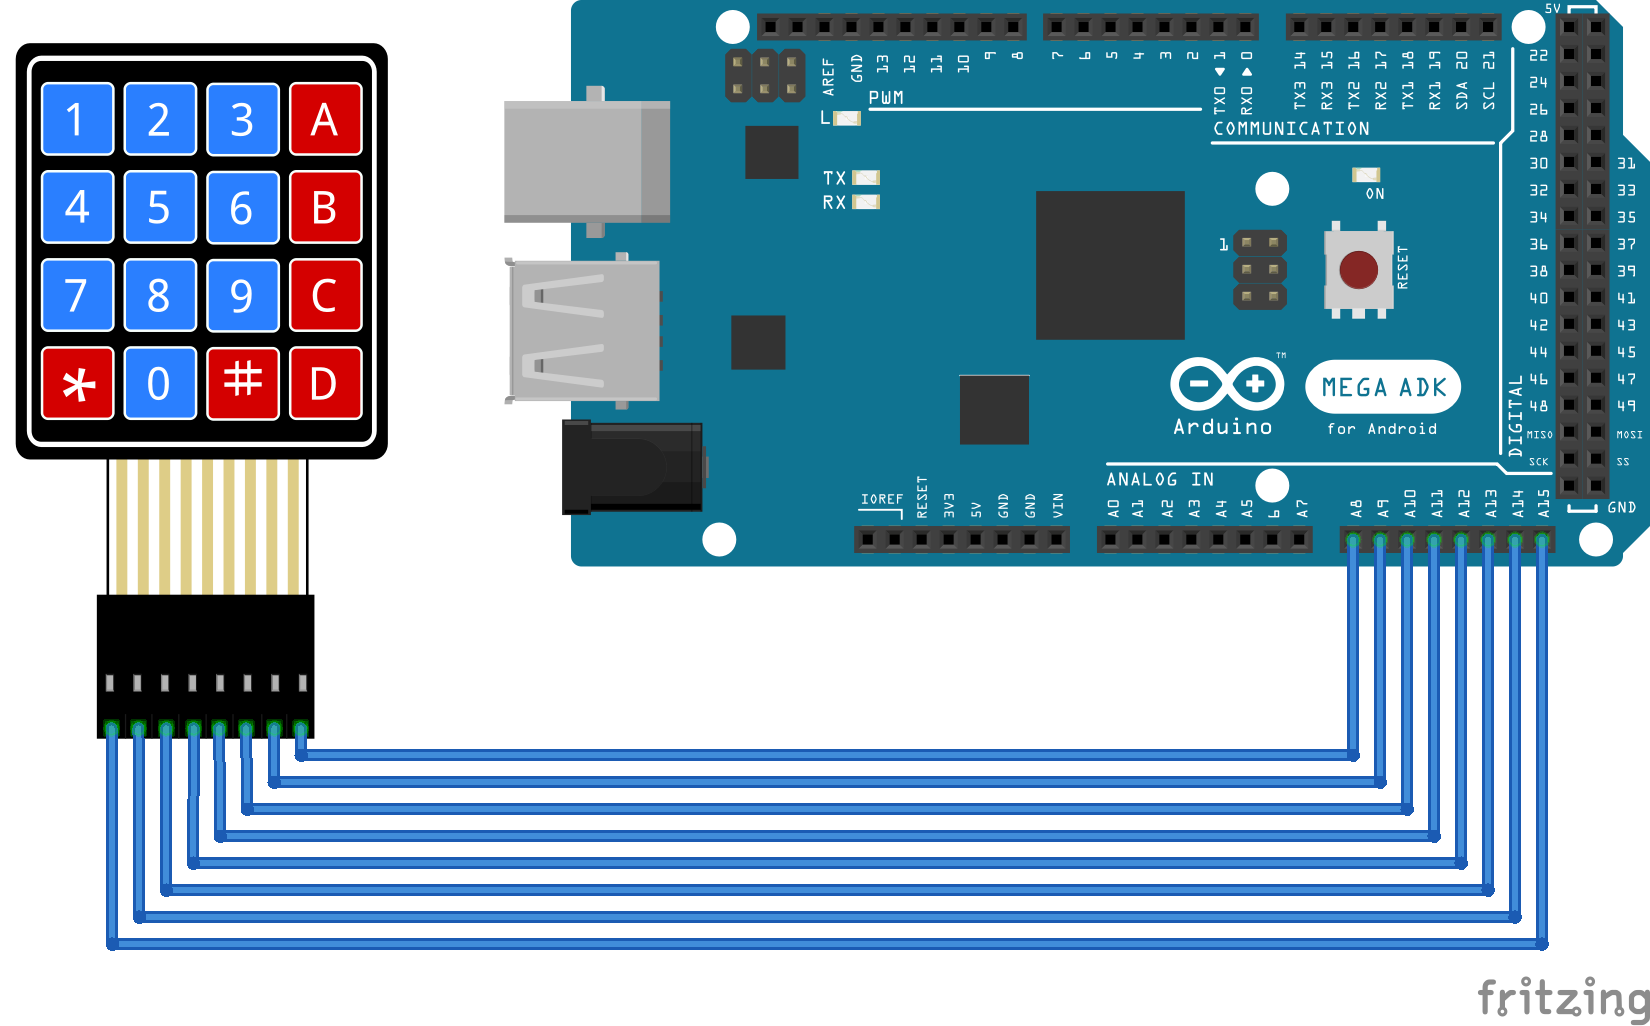
\includegraphics[width=0.5\textwidth]{figures/keybord_bb.png}
\caption{Keypad connection to Arduino}
\label{keyboard}
\end{figure}
Figure \ref{keyboard} represents the connection of 4*4 matrix keyboard to Arduino.

\subsection{Displaying Data}
We used a 16*2 liquid crystal display in this system to display the data. Slot status, parked or unparked or any other state.

\begin{figure}[H]
\centering
\subfloat[Display Connected to Arduino]{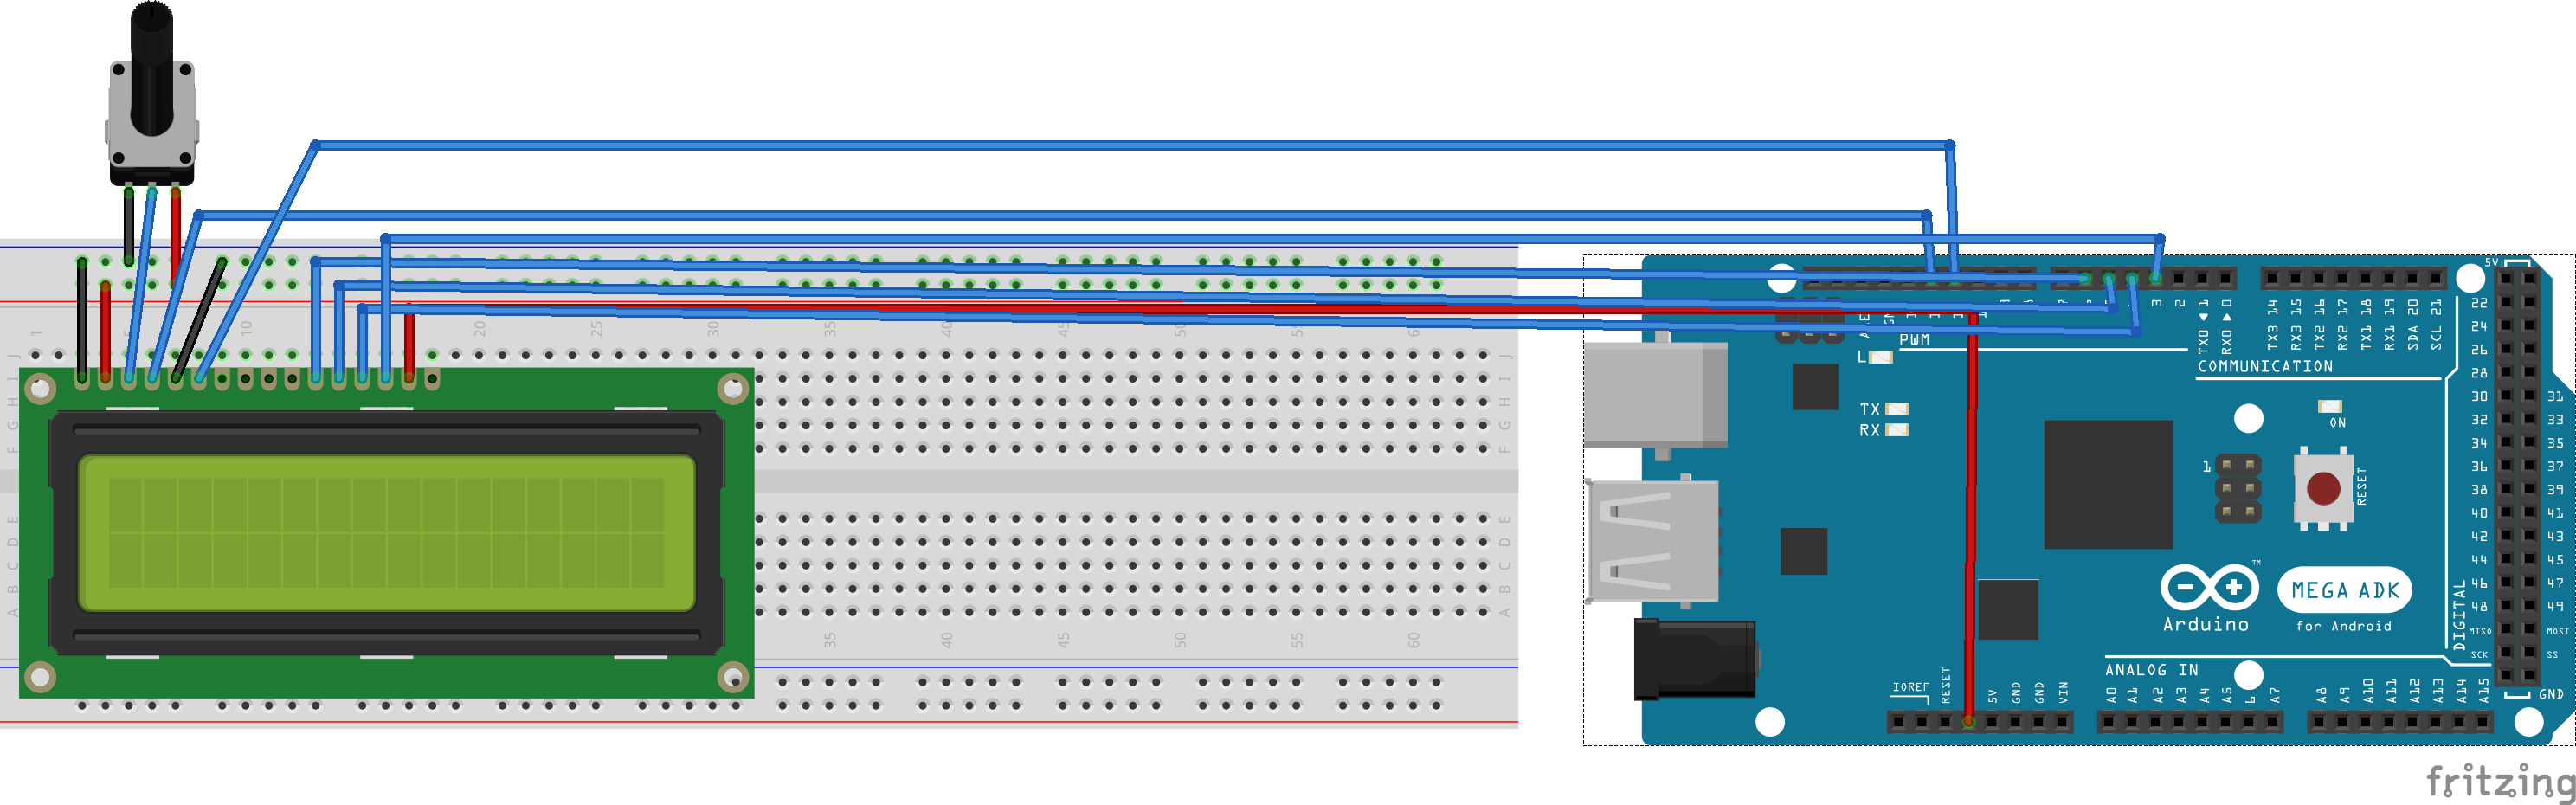
\includegraphics[width = 0.8\textwidth]{figures/display_bb.png}
\label{display1}} 
\hspace{1in}
\vspace{1cm}
\subfloat[Displaying Status]{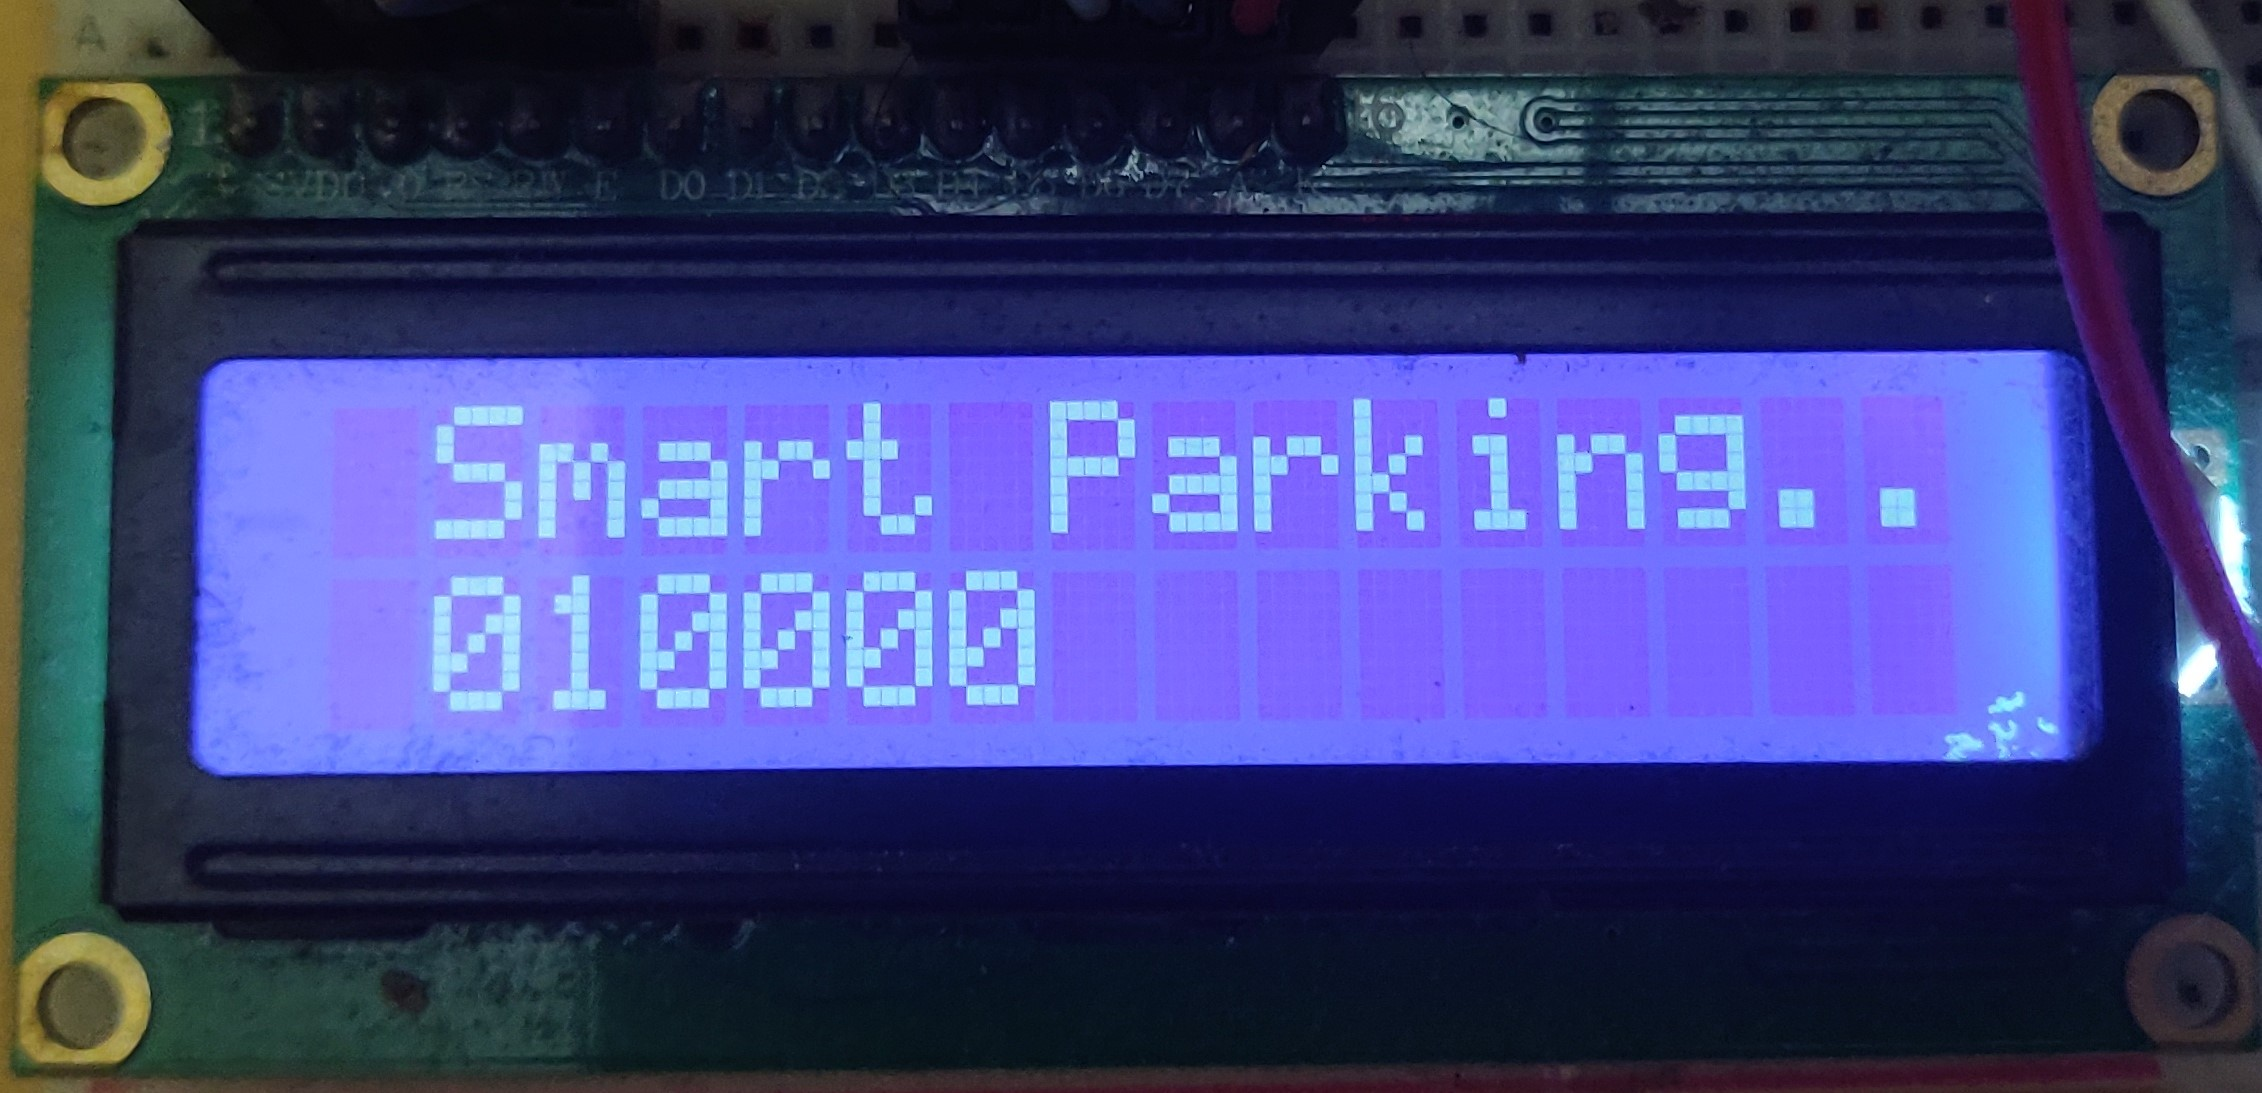
\includegraphics[width = 0.4\textwidth]{figures/display.jpg}
\label{display2}}
\caption{LCD Display}
\end{figure}

Figure \ref{display1} represents the connection of 16*2 liquid crystal display to Arduino. In figure\ref{display2} displaying slot status. Here '0' means the slot is free and '1' means that slot is not free.

\subsection{Making early alarm}
We used buzzer to make anti theft alarm. If a user parked car at a slot in server and in his profile it is updated that car is parked. If user does not request for unpark to server from his application but someone tries to place or steal car from parked state, this system considers that stealing is going on and an early alarm will be given. 
\begin{figure}[H]
\centering
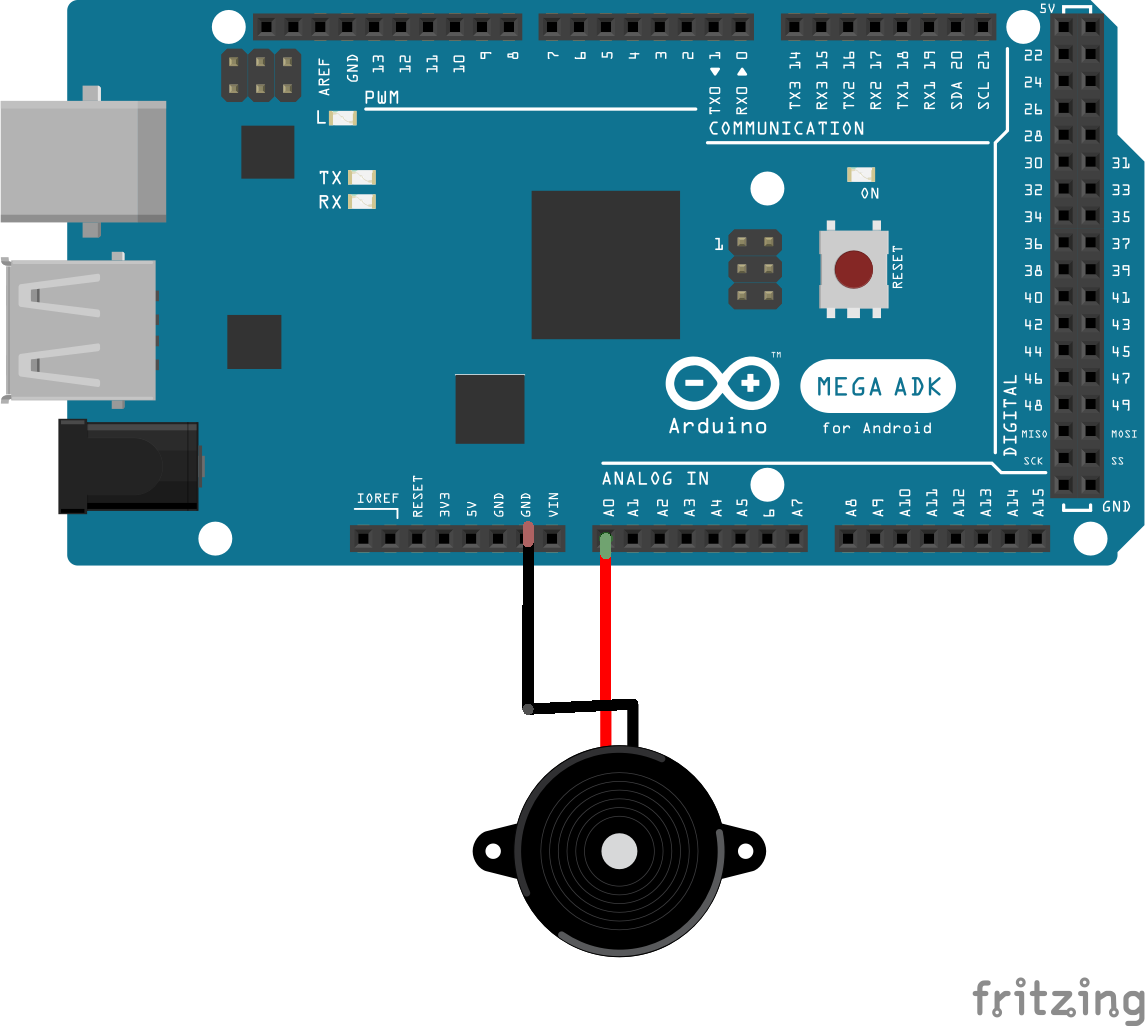
\includegraphics[width=0.5\textwidth]{figures/buzzer_bb.png}
\caption{Buzzer connection to Arduino}
\label{display}
\end{figure}
Figure \ref{display} represents the connection of alarm making buzzer to Arduino.

\subsection{Controlling Gate}
We used a main gate for parking spot. we used different servo motor for each slot. Gates are controlled by servo motor. If user request for a slot and pin is matched then gate is opened for a certain amount of time for parking the car. Again when user request for unpark the car. gates are opened for a certain amount of time to unpark the car.
\begin{figure}[H]
\centering
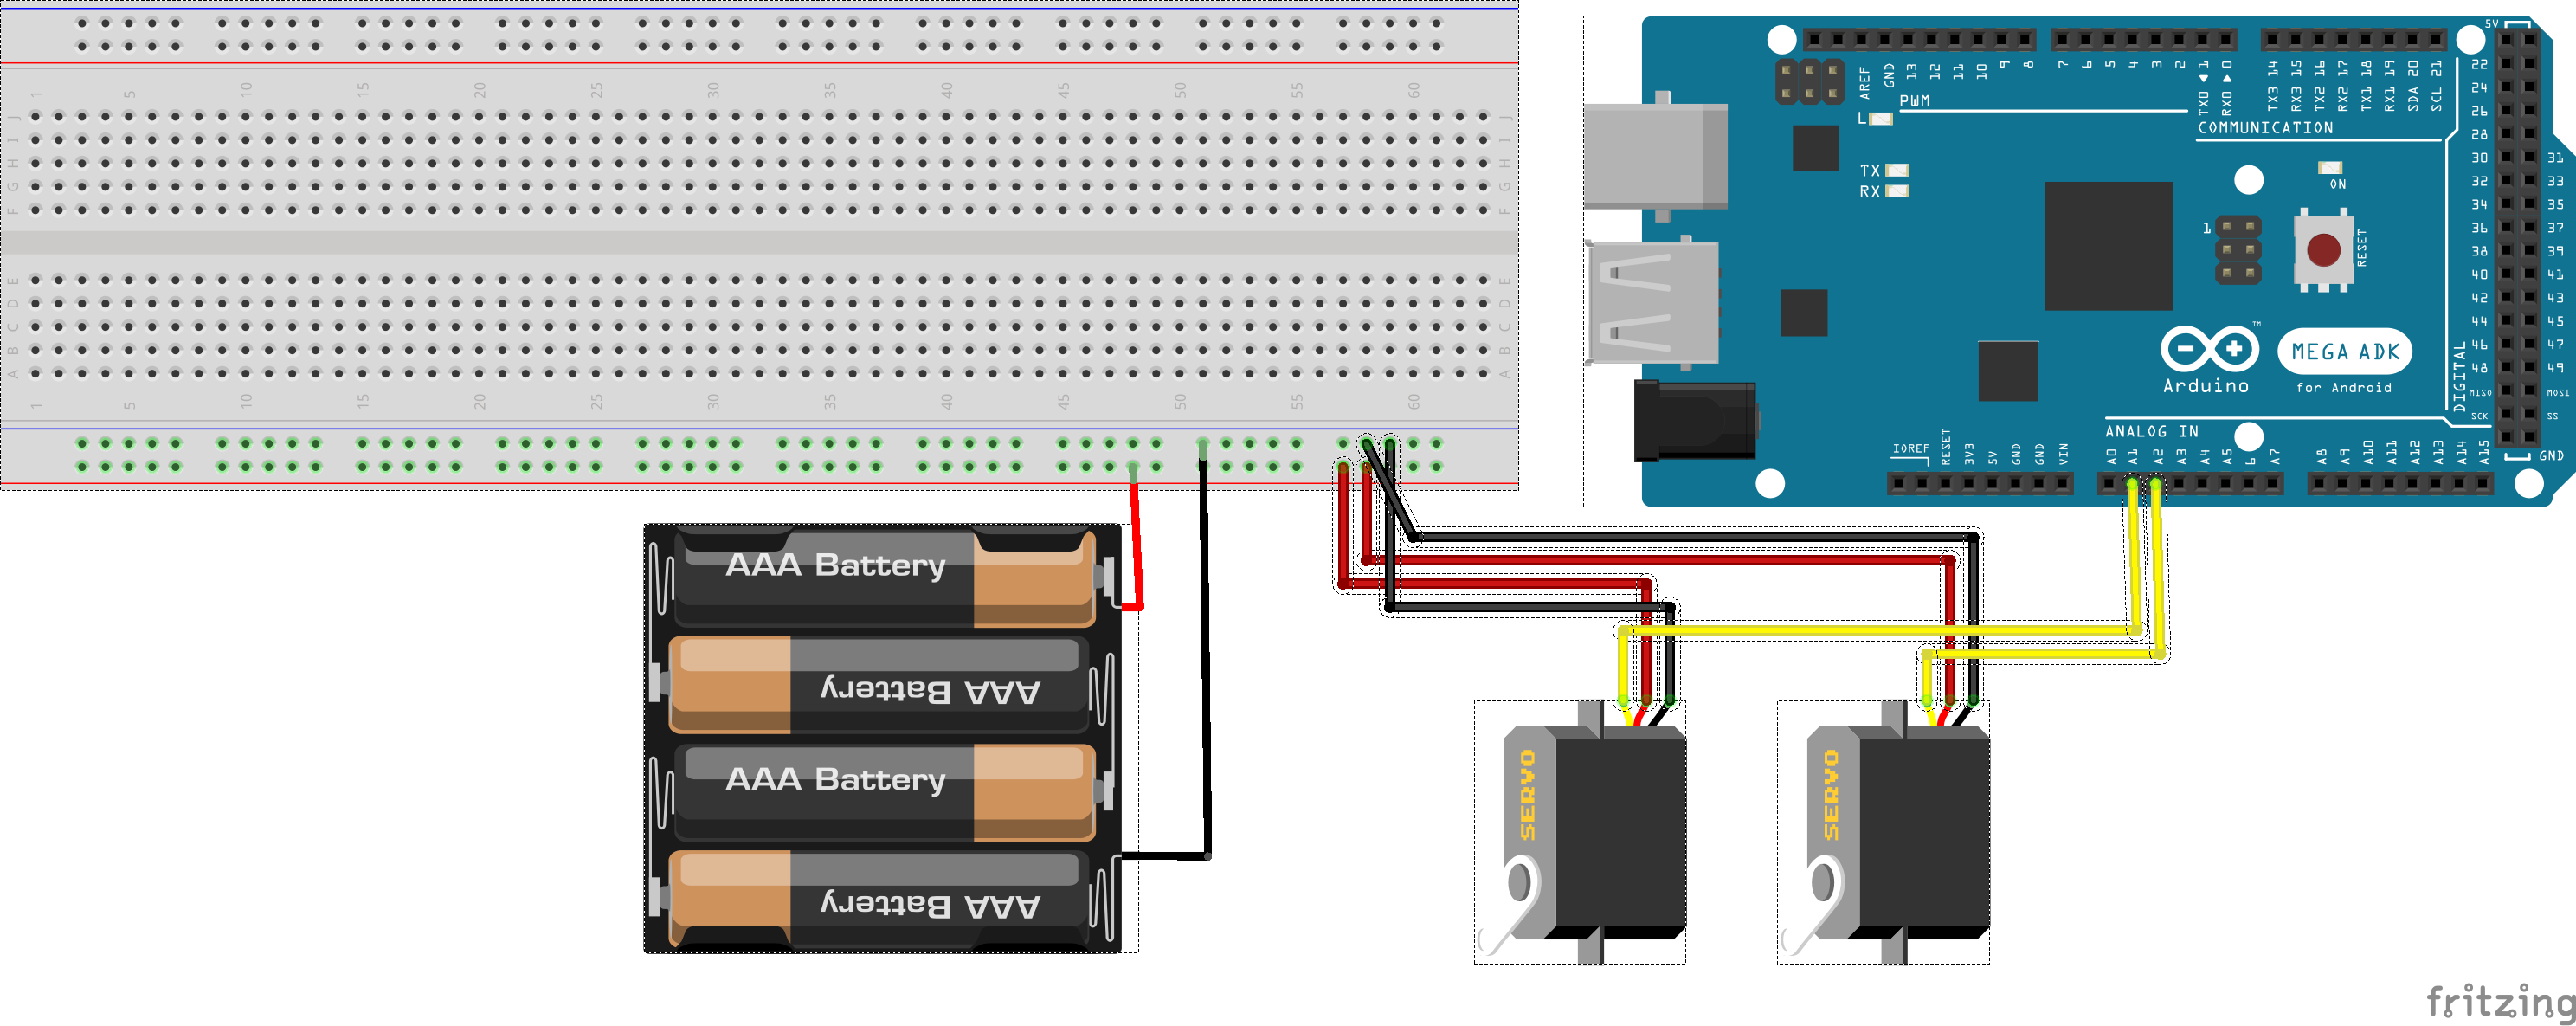
\includegraphics[width=0.5\textwidth]{figures/servo_bb.png}
\caption{Servo Motor Connection to Arduino}
\label{servo}
\end{figure}
Figure \ref{servo} represents the connection of servo motor to Arduino as gate.

\subsection{SMS sending with GSM Mdoule}
We used SIM900 GSM module for sending SMS to respective person. When the system found that someone is stealing car, it makes an early alarm and send an alarming SMS to the respective person with this module.

\begin{figure}[H]
\centering
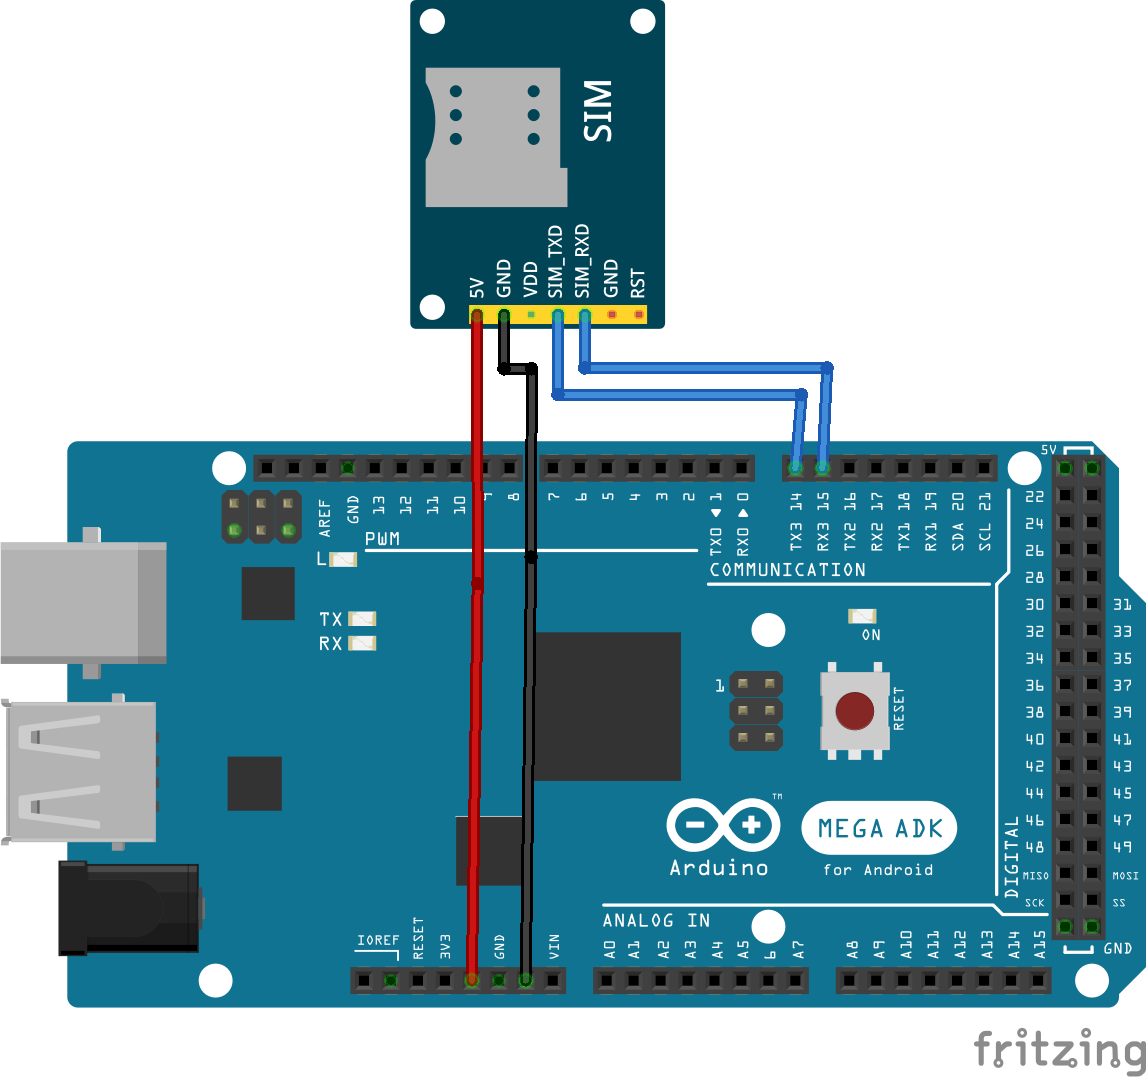
\includegraphics[width=0.5\textwidth]{figures/gsm_bb.png}
\caption{GSM Module Connection to Arduino}
\label{gsm}
\end{figure}
Figure \ref{gsm} represents the connection of SIM900 GSM module to Arduino.

\subsection{Android Application as Interacting interface}
We developed android application to interact with this system. Figure \ref{icon} is the android application icon. Figure \ref{login1} is the login interface. For only one time user has to enter the phone number and car serial. Figure \ref{login2} represents that information is save and profile is created. After profile is created every time user launch the app it login automatically using saved information. Figure \ref{profile} represents that on firebase database cloud server a profile in his information is created.

\begin{figure}[H]
\centering
\subfloat[Android Application Icon]{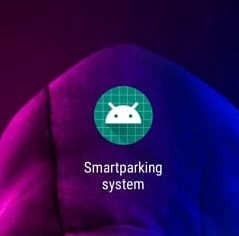
\includegraphics[width = 0.4\textwidth]{figures/app_icon.jpg}
\label{icon}} 
\hspace{1cm}
\subfloat[Profile Creating on Server]{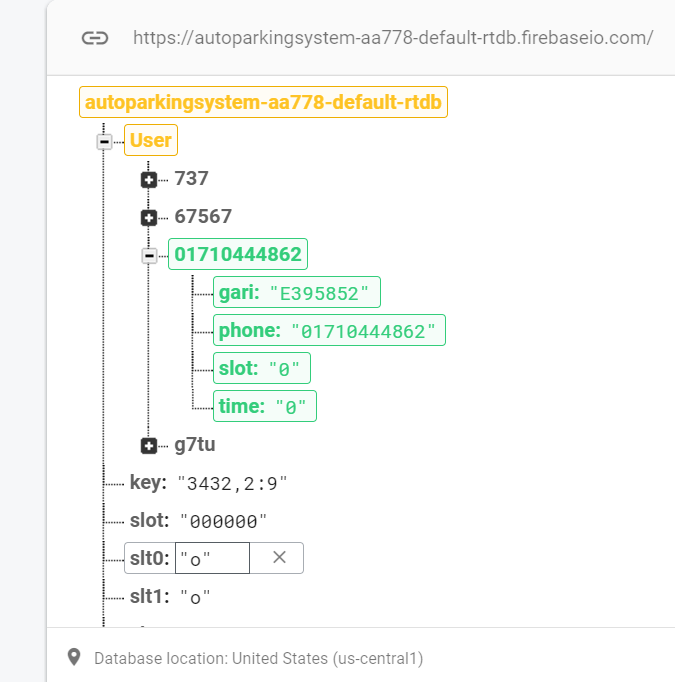
\includegraphics[width = 0.4\textwidth]{figures/profile_s.png}
\label{profile}}
% \caption{Login Interface and Profile Creation}
\end{figure}

\begin{figure}[H]
\centering
\subfloat[Login Page]{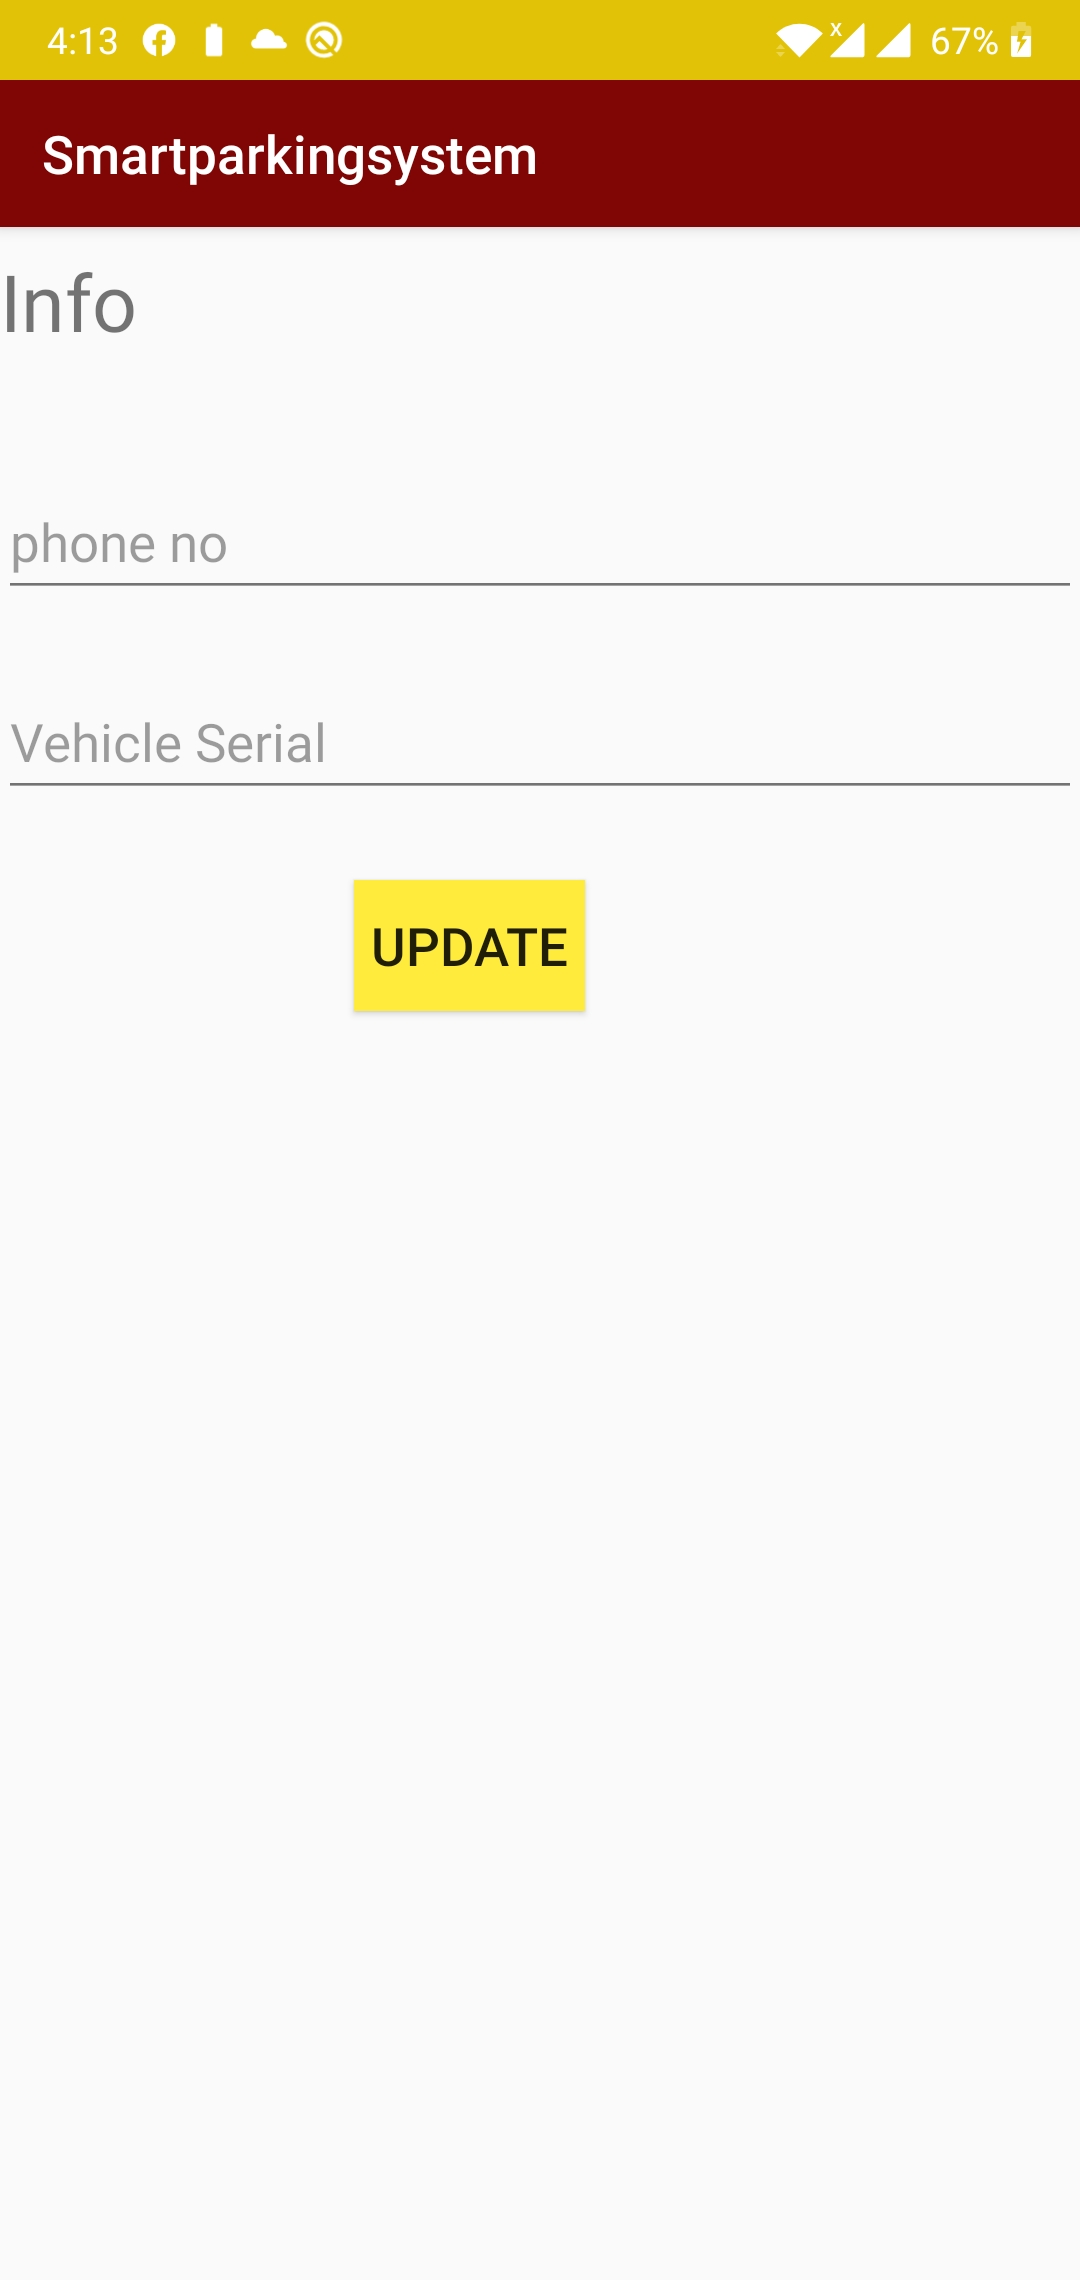
\includegraphics[width = 0.35\textwidth]{figures/home_m.jpg}
\label{login1}} 
\hspace{1cm}
\subfloat[Information Saved]{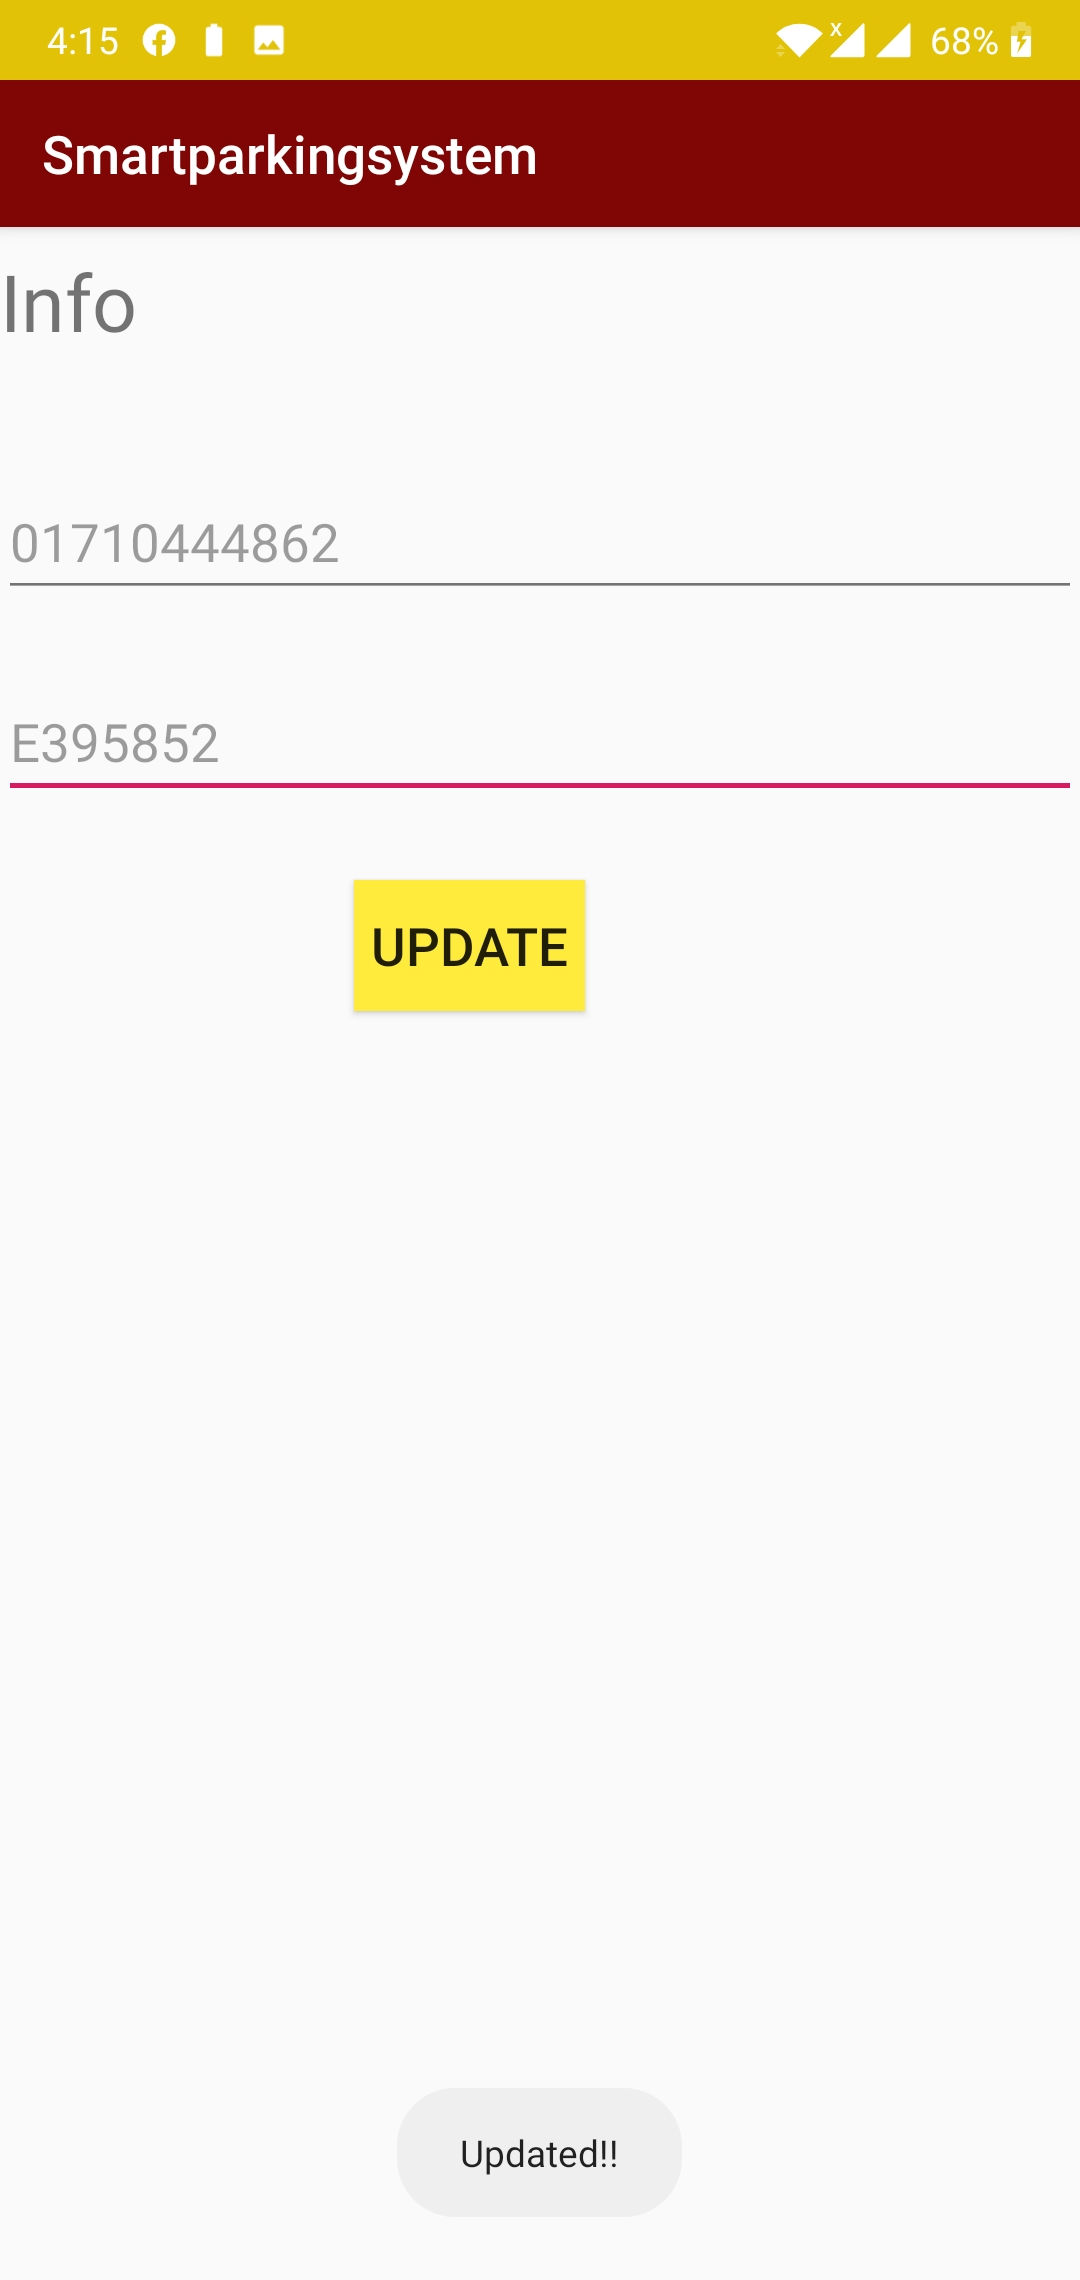
\includegraphics[width = 0.35\textwidth]{figures/profile_m.jpg}
\label{login2}}
\caption{Login Interface and Profile Creation}
\end{figure}




% \begin{figure}[H]
% \centering
% \subfloat[Android Application Icon]{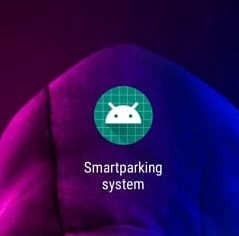
\includegraphics[width = 0.4\textwidth]{figures/app_icon.jpg}
% \label{icon}} 
% \hspace{1cm}

% \subfloat[Login Page]{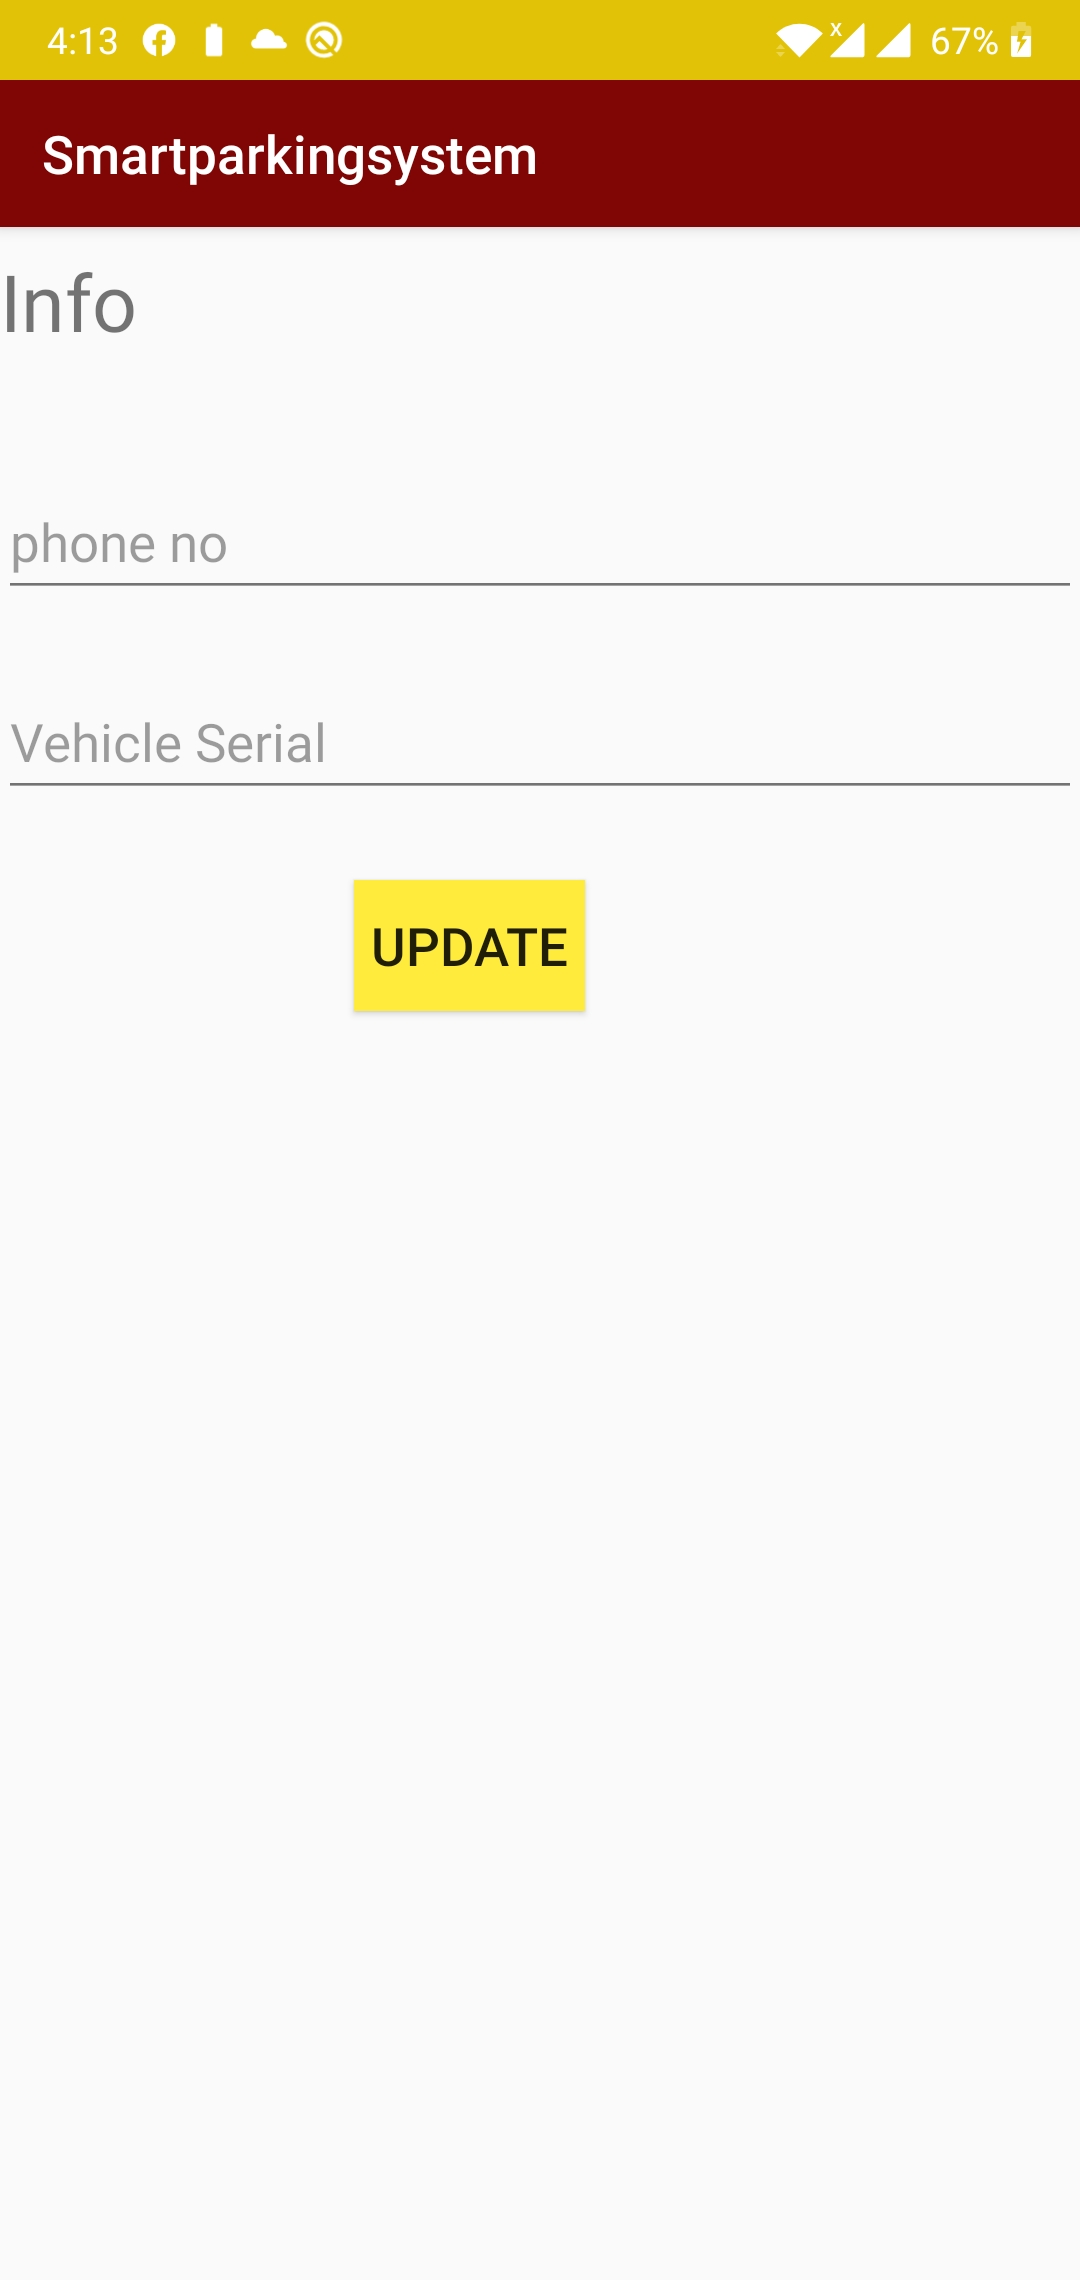
\includegraphics[width = 0.3\textwidth]{figures/home_m.jpg}
% \label{login1}}
% \hspace{1cm}
% \subfloat[Login Page]{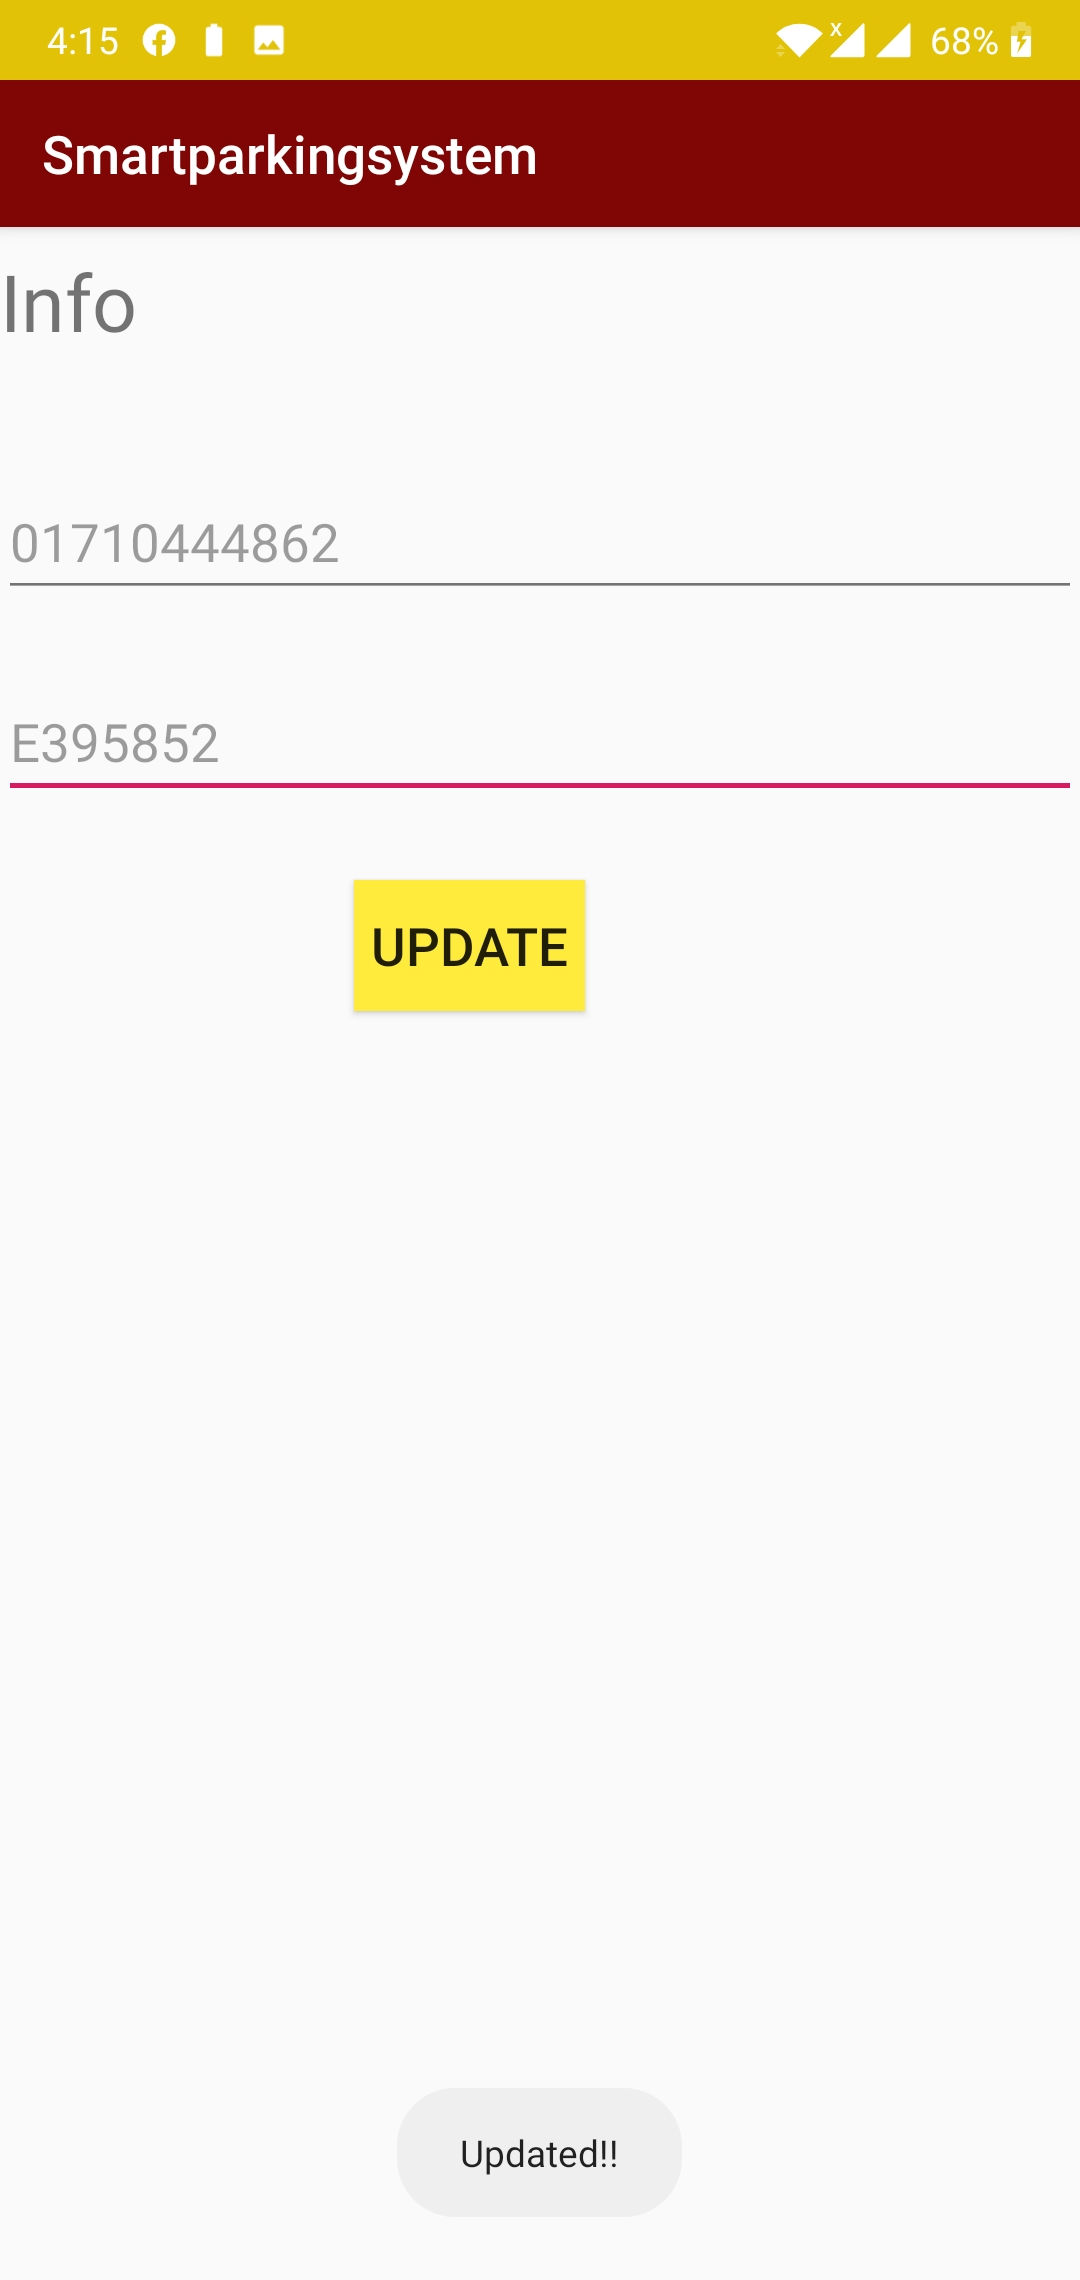
\includegraphics[width = 0.3\textwidth]{figures/profile_m.jpg}
% \label{login2}}
% \hspace{1cm}

% \subfloat[Login Page]{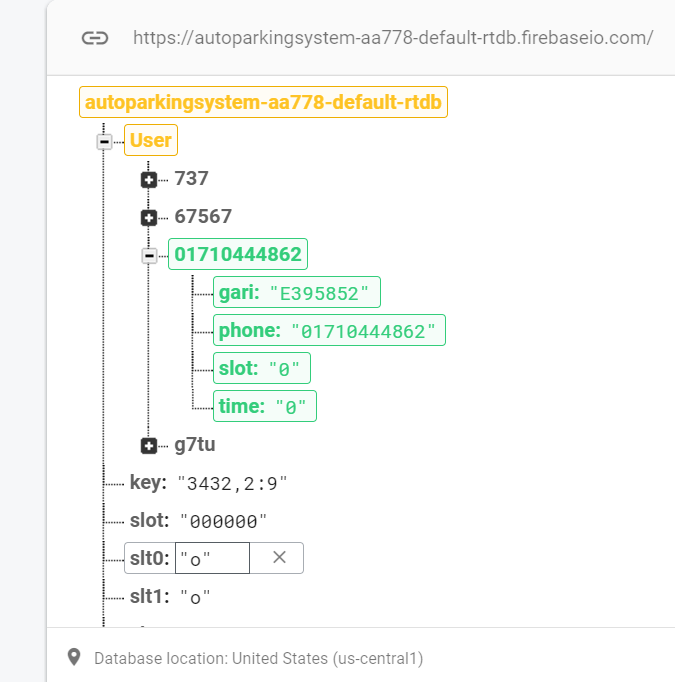
\includegraphics[width = 0.3\textwidth]{figures/profile_s.png}
% \label{profile}}
% \caption{Login Interface and Profile Creation}
% \end{figure}

\section{Implementation}
Here we will discuss on the implementation of hardware, software, application and features.

\subsection{Required Hardware:}
In our system we have used the following hardware components. These hardware components have been selected since they are relatively cheaper than others. At the testing stage, the viability of our suggested system is successfully determined by employing these components.
\begin{itemize}
    \item Arduino
    \item GSM module
    \item Display
    \item Keypad
    \item IR obstacle sensor
    \item Buzzer
    \item Servo motor
    \item NodeMCU
\end{itemize}
\subsection{Required Software:}
In our system we have used the following softwares.
\begin{itemize}
    \item Arduino IDE
    \item Android Studio
    \item Firebase
    \item Web Browser
\end{itemize}
\subsection{Required Programming Language:}
\begin{itemize}
    \item C
    \item Python
    \item Extensive markup language (XML)
    \item JAVA
\end{itemize}

\subsection{Emergency and Non Emergency Parking Slot}
In figure \ref{type1} we see two button for emergency slot and non emergency slot. Requesting for emergency slot does not required any pin verification but for non emergency slot pin verification is needed which will be discussed in the following section. Emergency slot has no servo controlled gate. Only the main gate will be opened at the time of parking. And for non emergency slot gate is there. At the time of parking at non emergency slot the main gate and slot gate is opened. Figure \ref{slottype} represents that the number 1 slot is emergency slot and others are non emergency slot.  

\begin{figure}[H]
\centering
\subfloat[Emergency and non Emergency Button]{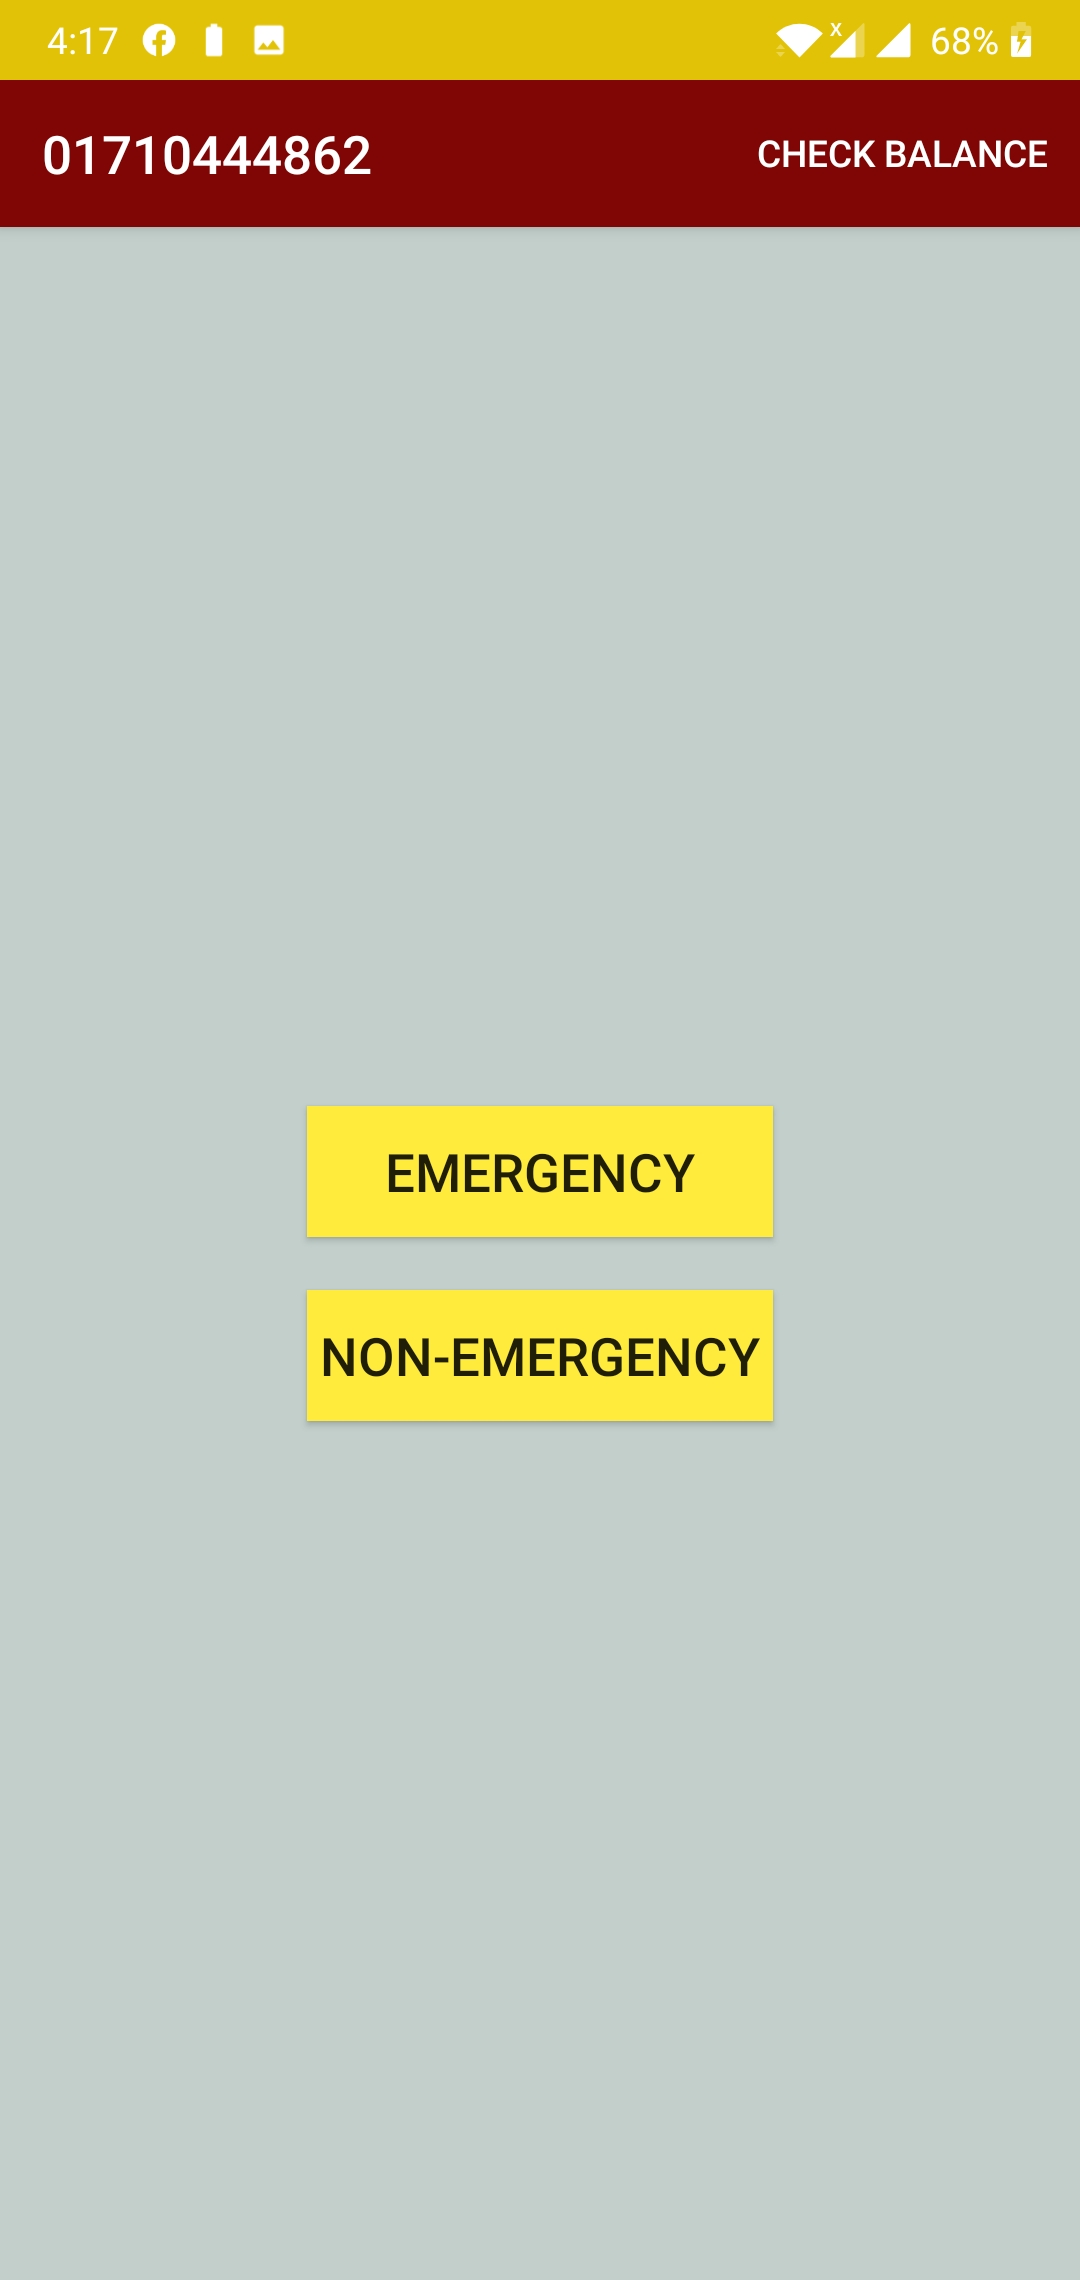
\includegraphics[width = 0.35\textwidth]{figures/slot_type_m.jpg}
\label{type1}} 
\hspace{1cm}
\subfloat[First is Emergency Slot]{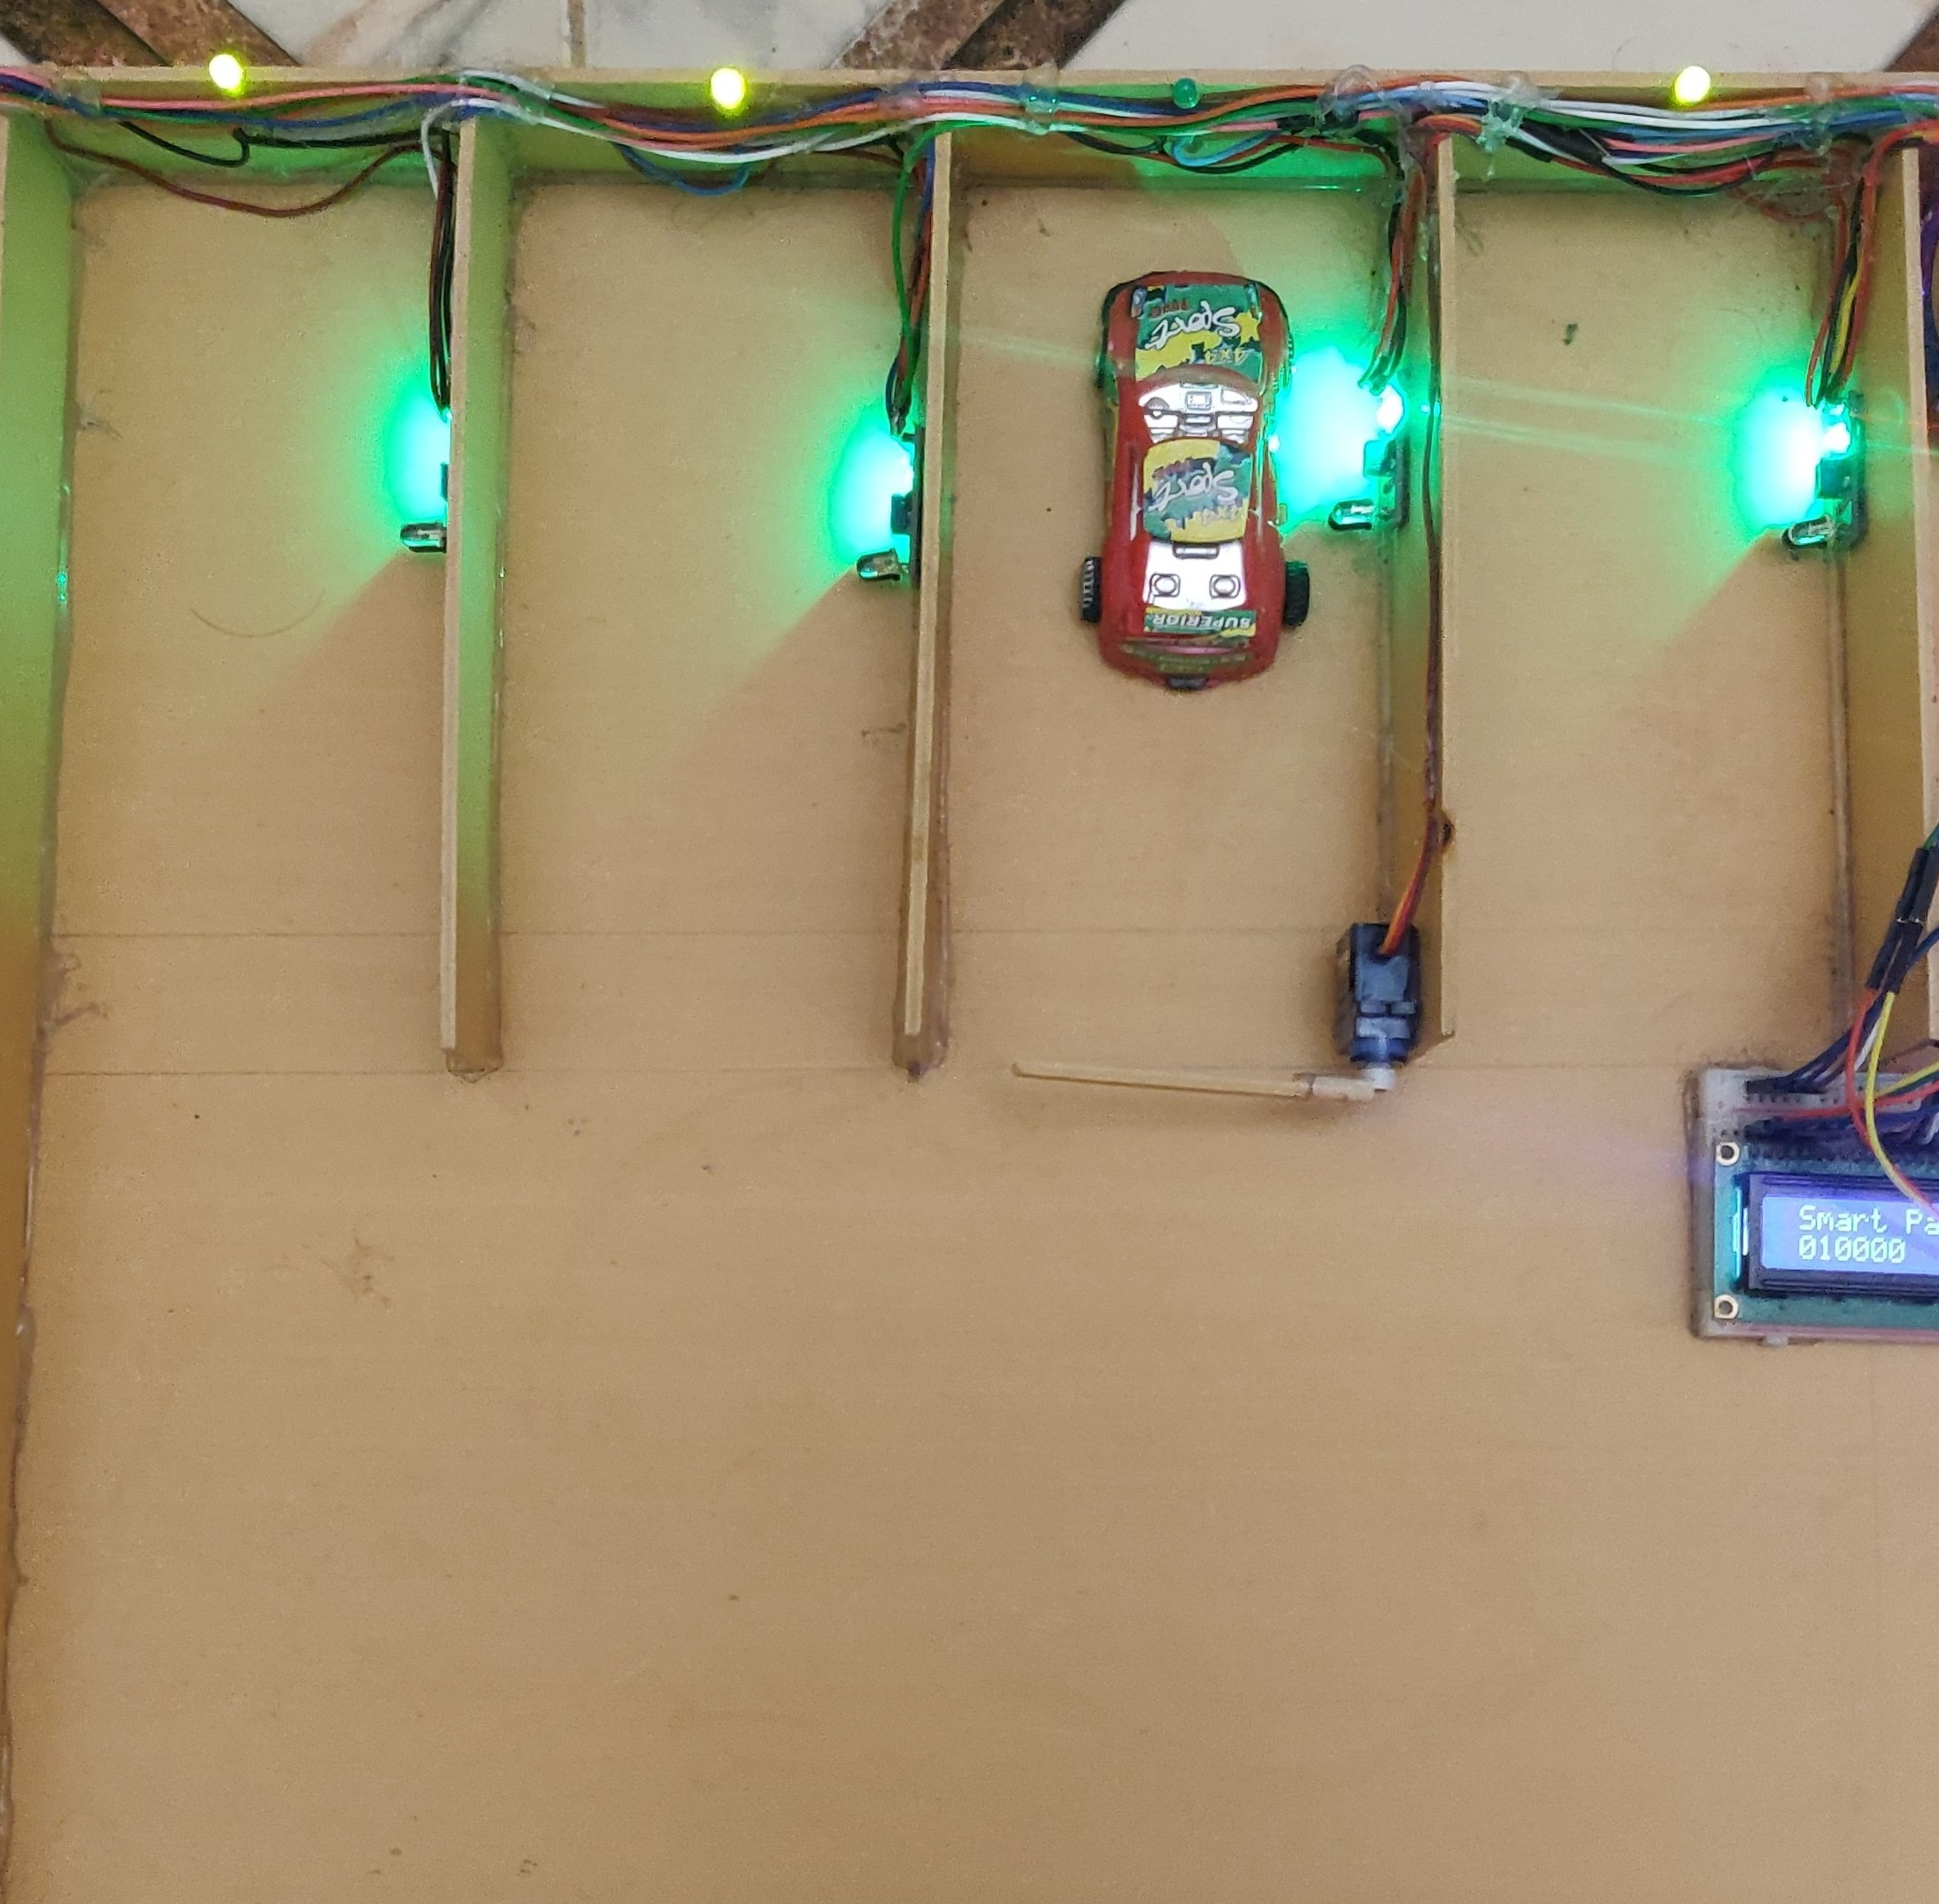
\includegraphics[width = 0.35\textwidth]{figures/E_ne.jpg}
\label{slottype}}
\caption{Emergency and non Emergency }
\end{figure}

\subsection{Requesting for a slot}
For emergency slot no submitting for slot number is needed. If "Emergency" button is pressed slot request will be sent to system. Thus there is no complexity for emergency slot, it is very easy and fast for parking. This slot is mainly designed for emergency vehicle such as ambulance. After requesting for emergency button if the car parked at emergency slot the time counting is started and on application it shows that at slot 1 car is parked \ref{e_parked}. For non emergency slot the slot number is to be submitted \ref{input_num}. 
% \begin{figure}[H]
% \centering
% 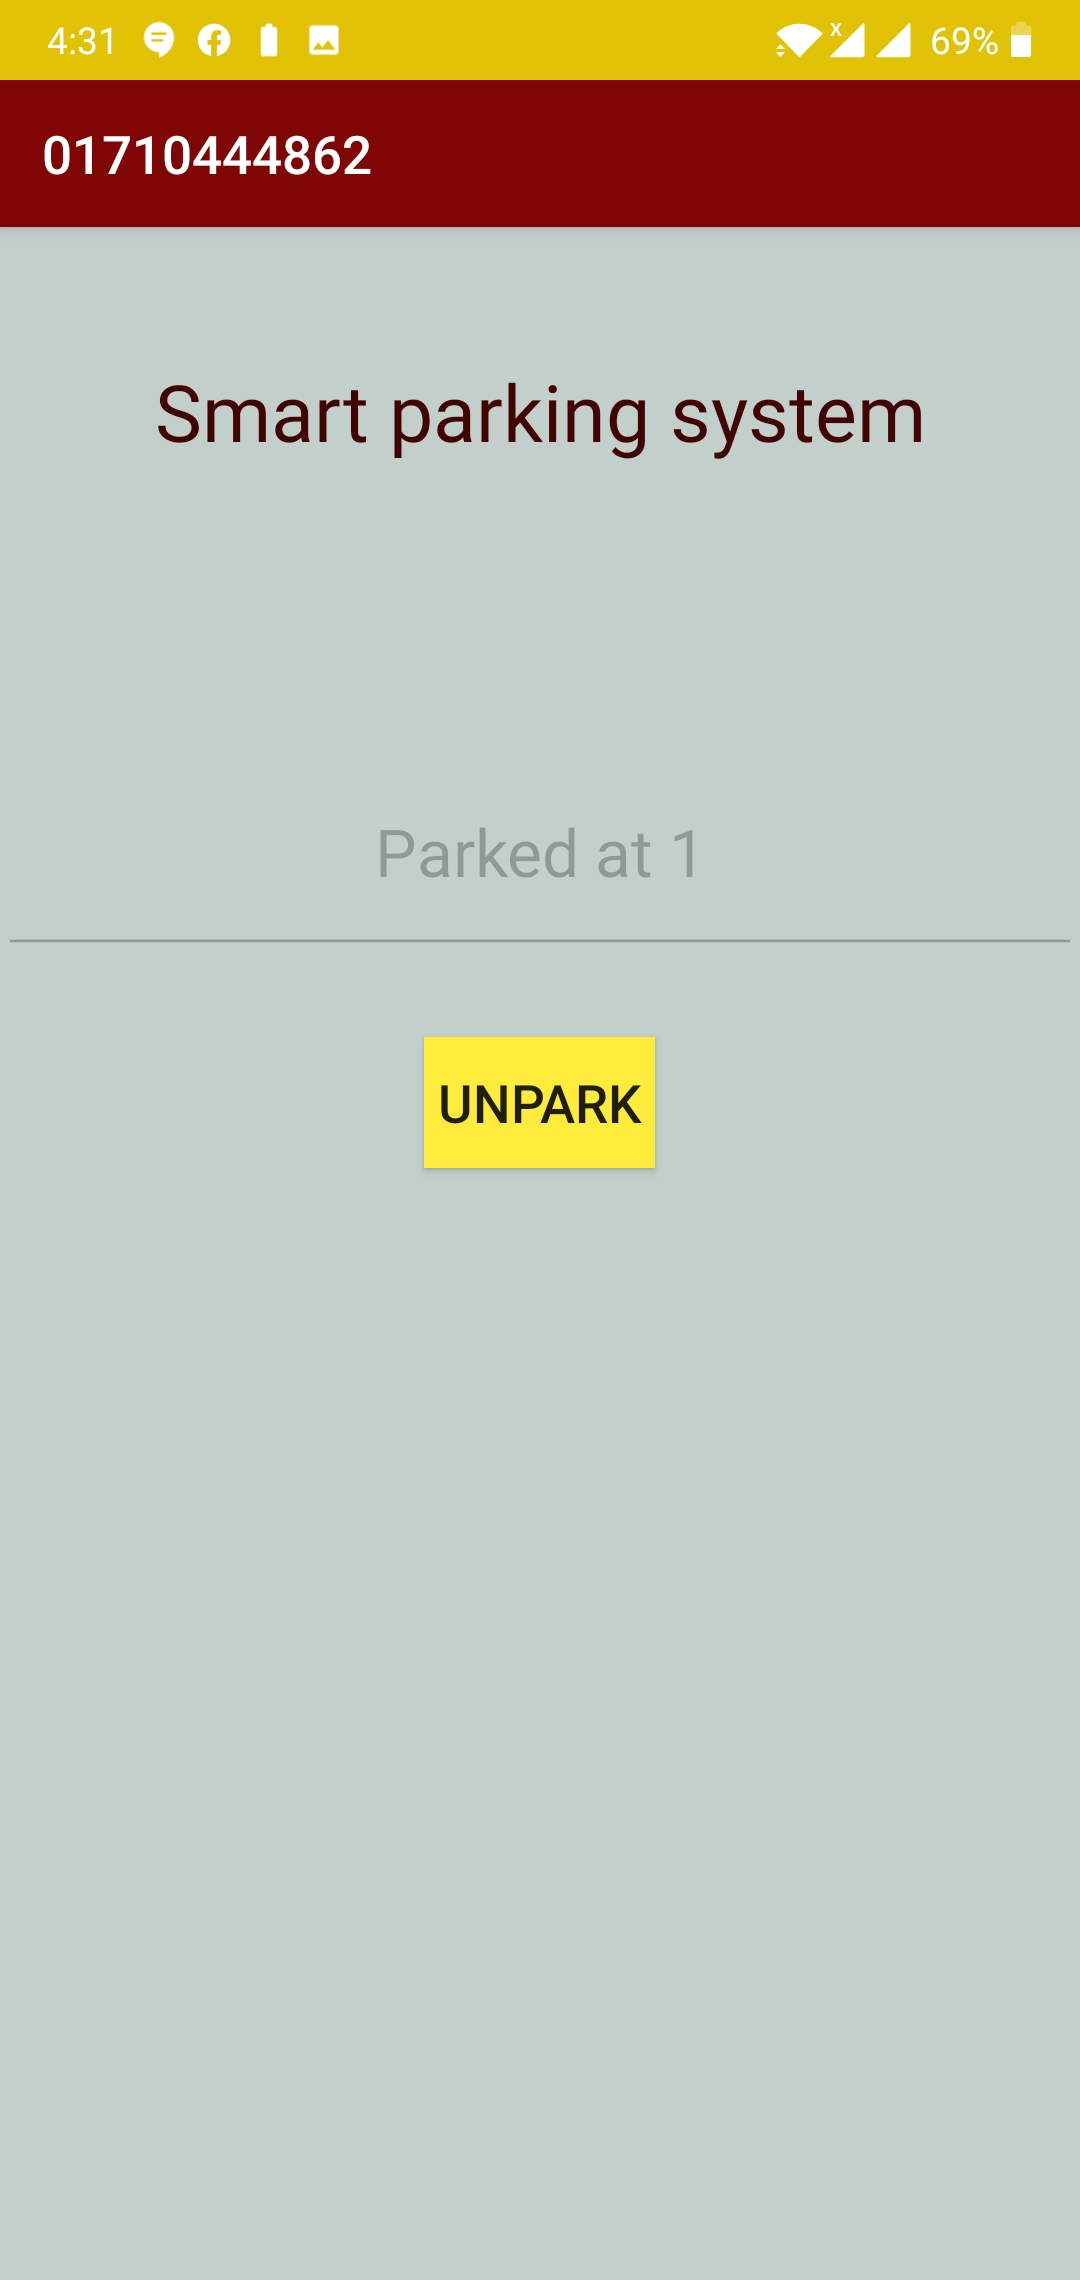
\includegraphics[width=0.5\textwidth]{figures/emergency_parked_m.jpg}
% \caption{Parked at Emergency Slot}
% \label{e_parked}
% \end{figure}

\begin{figure}[H]
\centering
\subfloat[Parked at Emergency Slot]{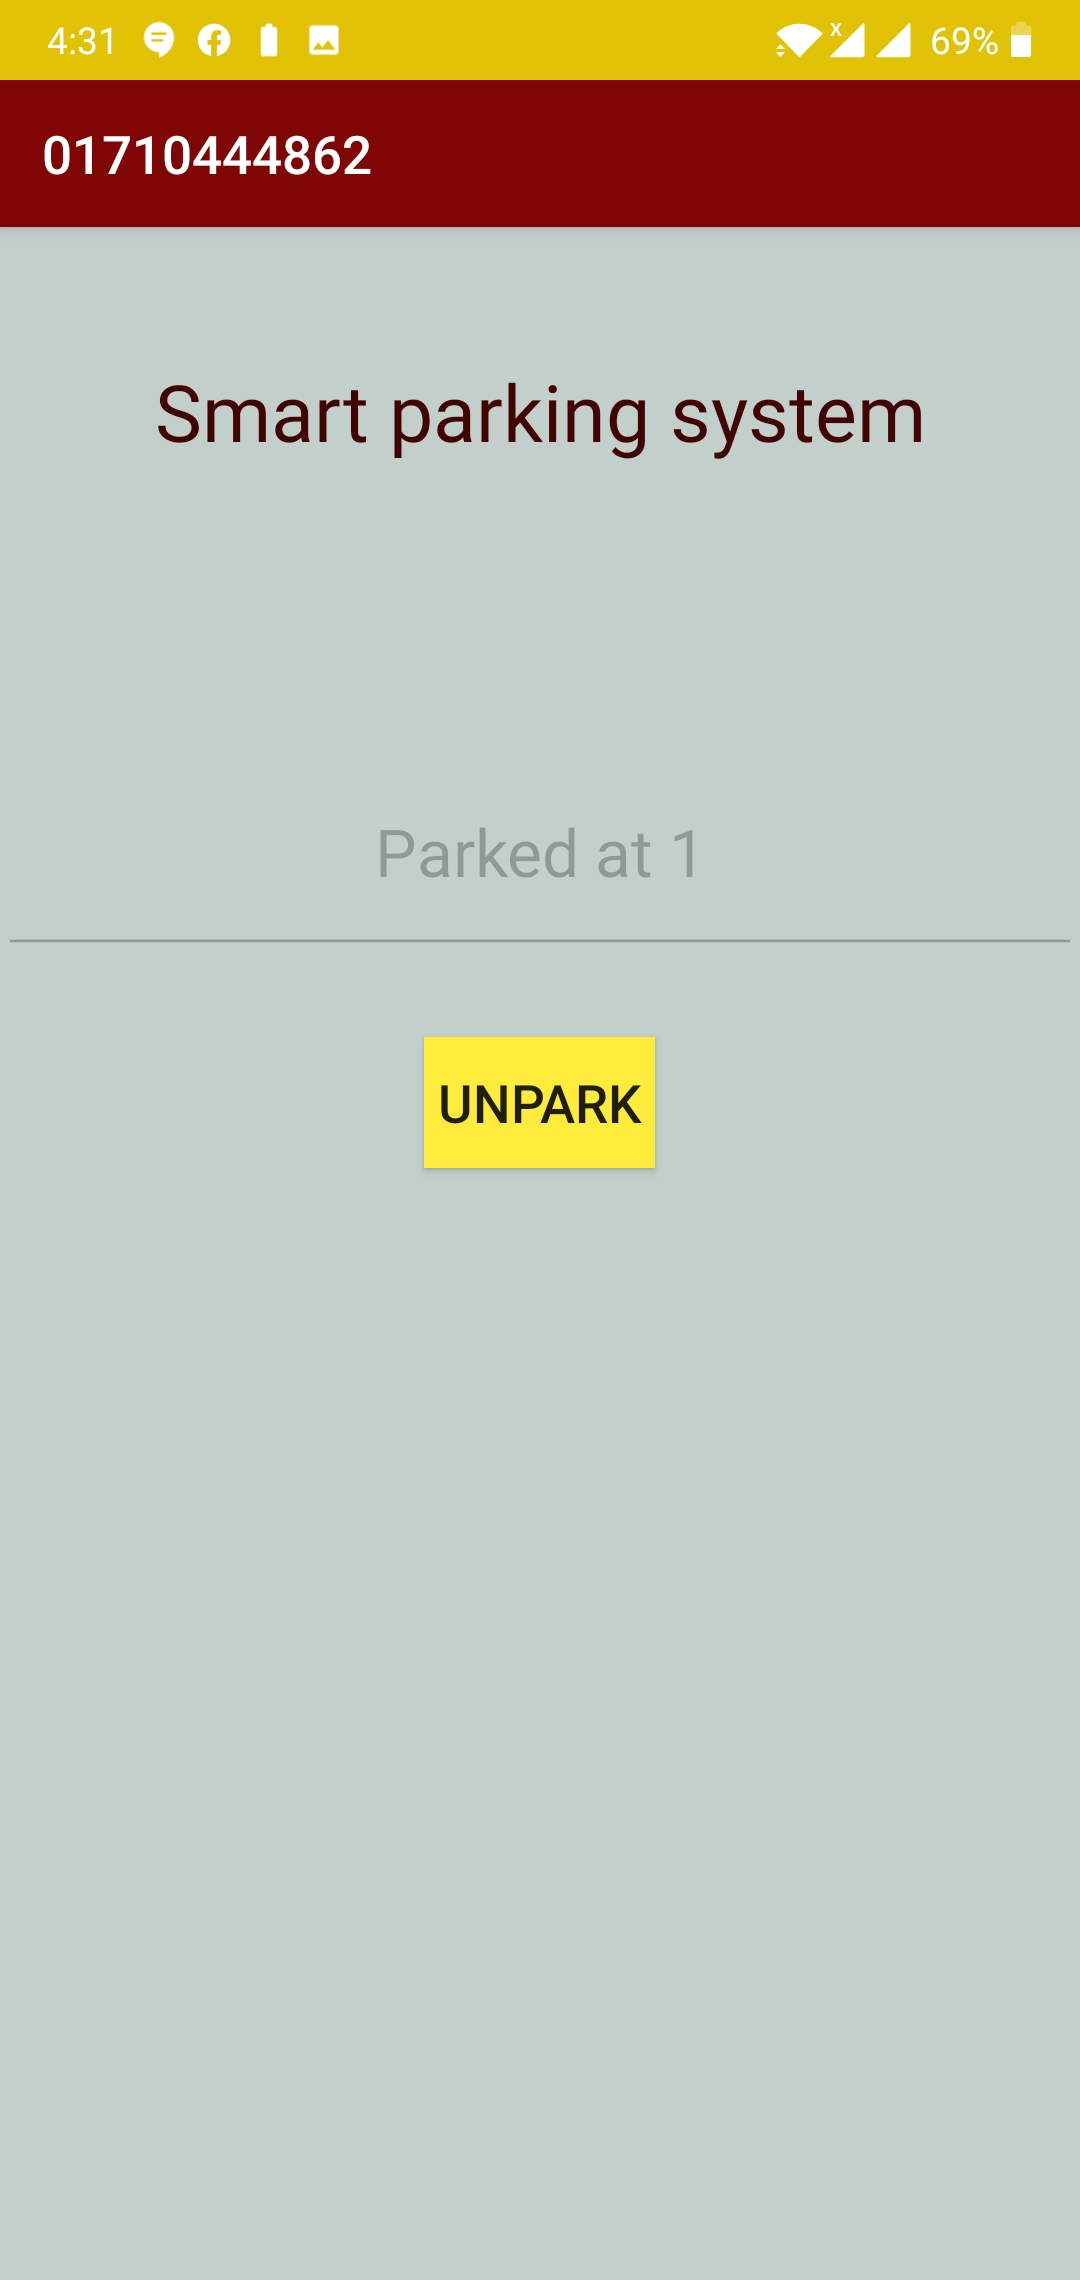
\includegraphics[width = 0.4\textwidth]{figures/emergency_parked_m.jpg}
\label{e_parked}}
\hspace{1cm}
\subfloat[Slot Number inputting]{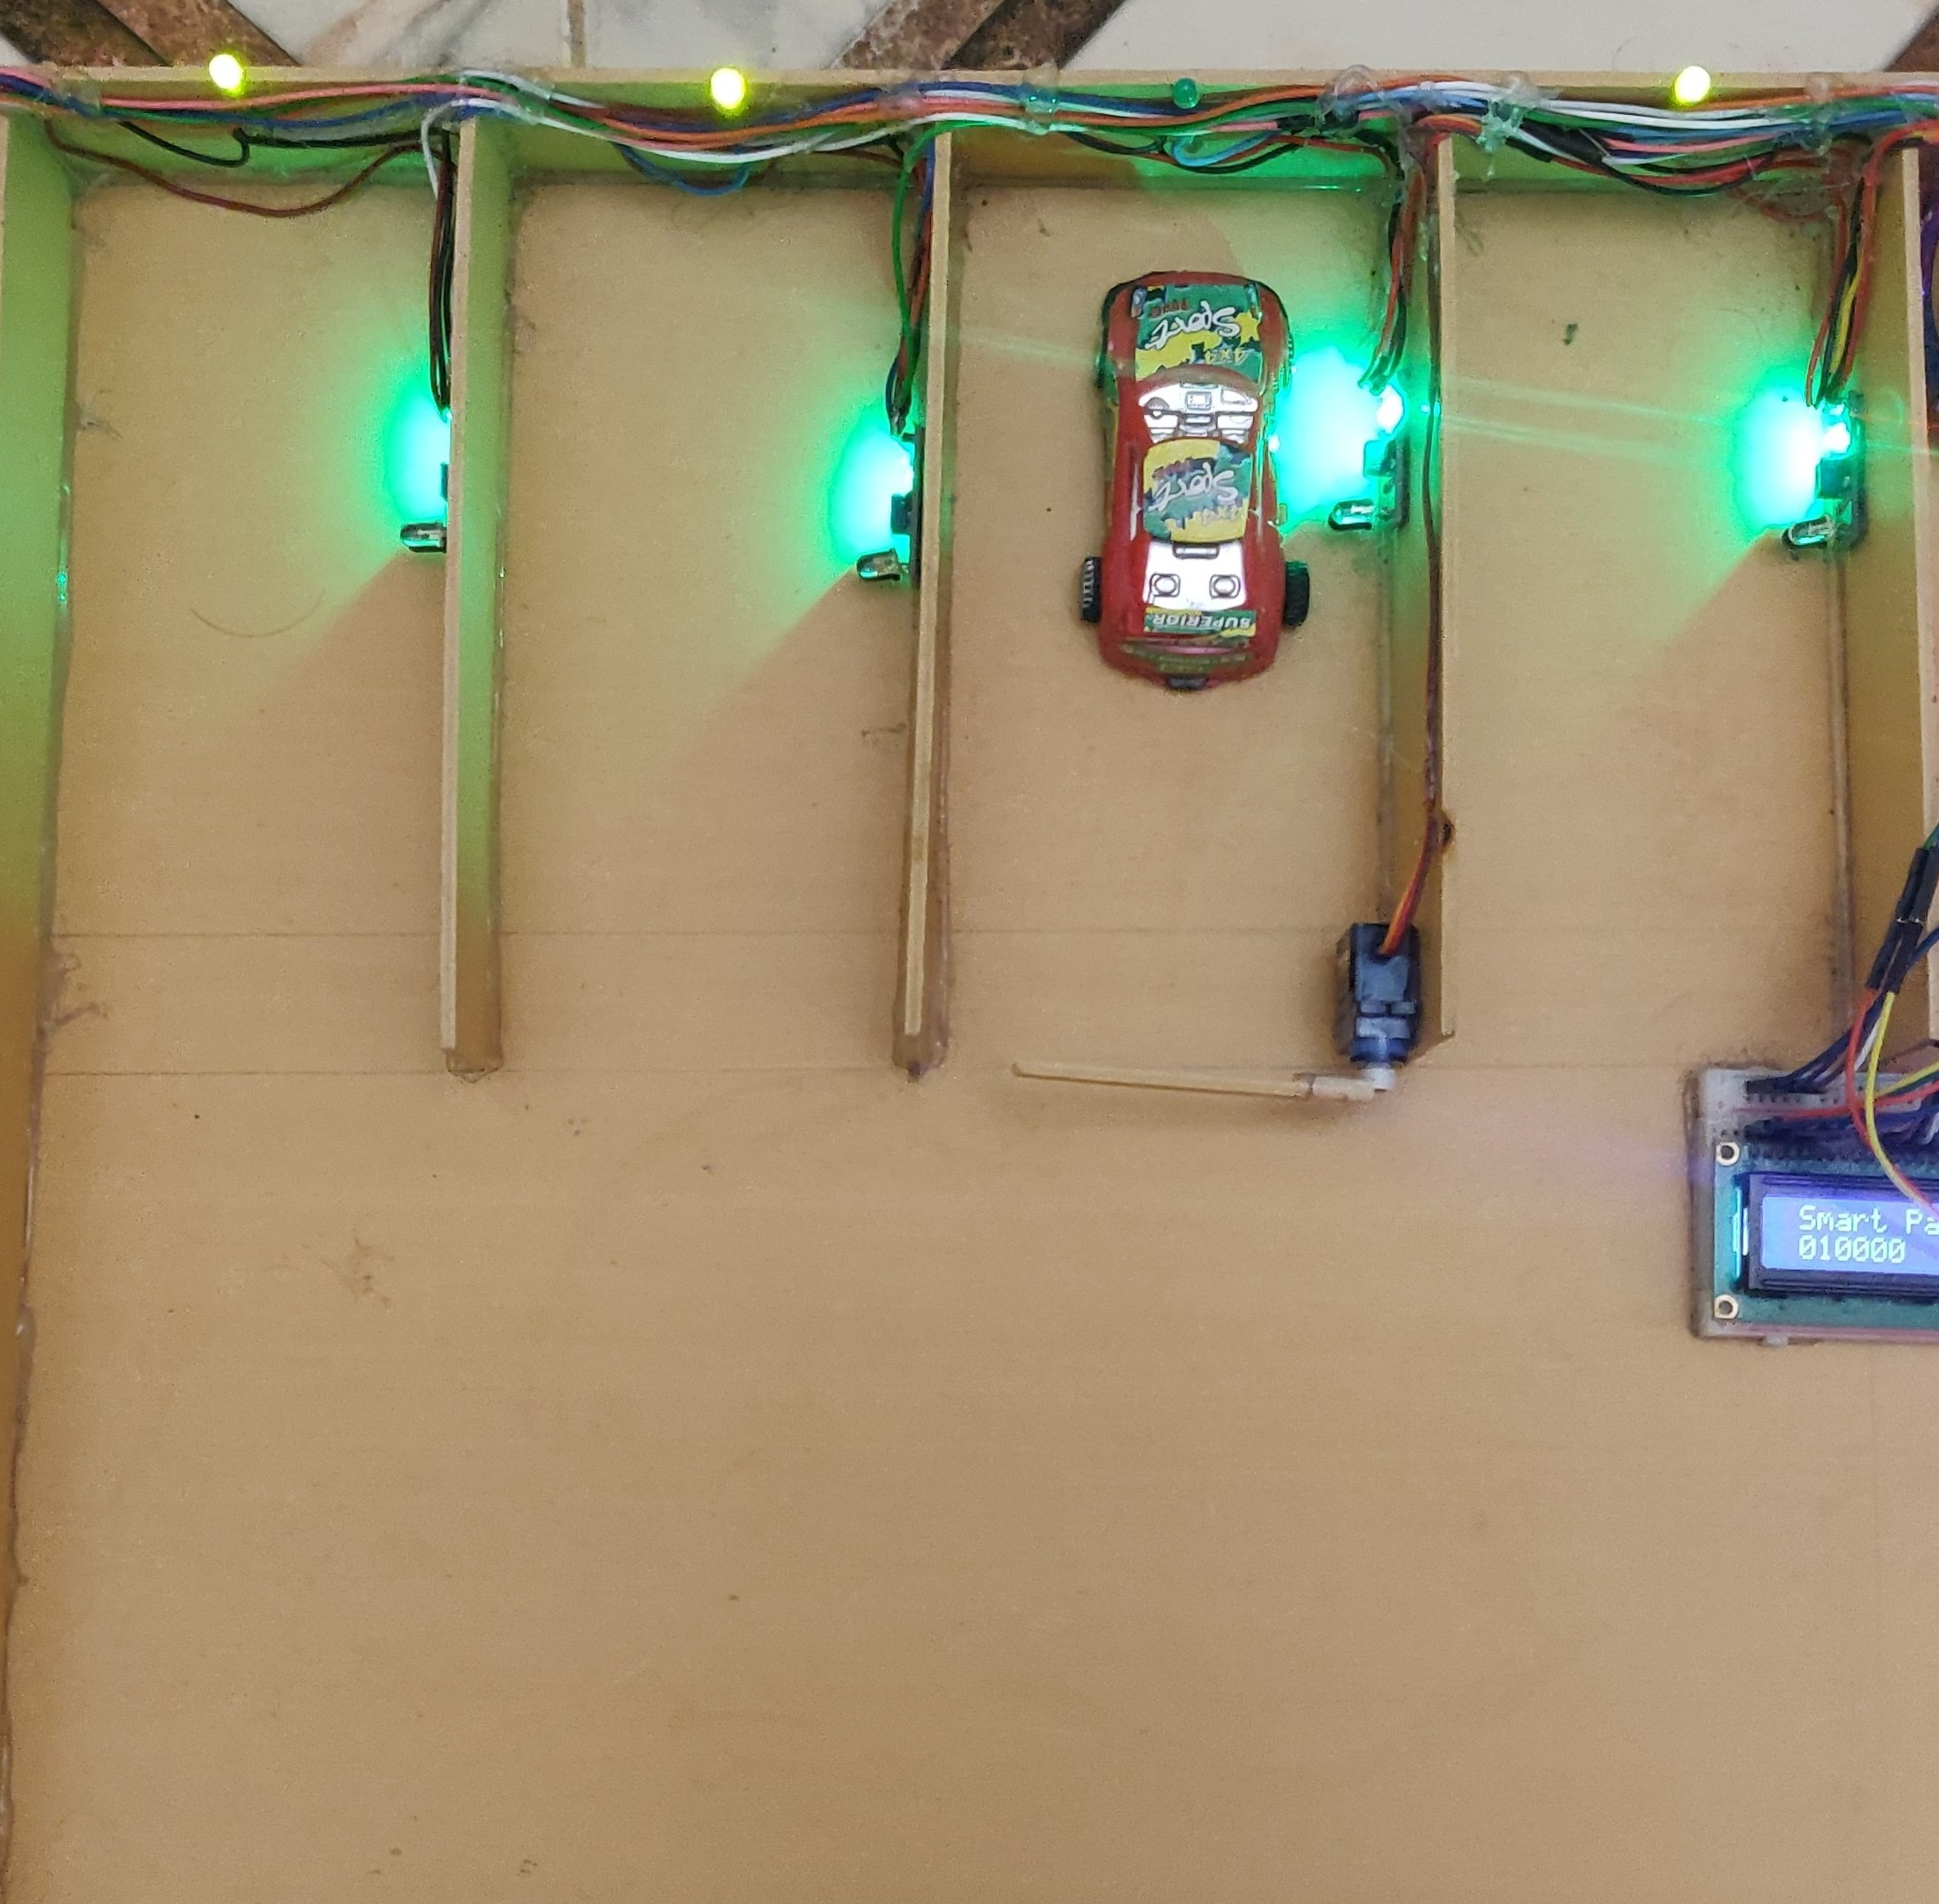
\includegraphics[width = 0.4\textwidth]{figures/E_ne.jpg}
\label{input_num}}
\caption{Submitting Slot Number }
\end{figure}

\subsection{Pin Verification and Slot Allocation}
When user requests for a slot from android application, a four digit pin code is generated and send to server \ref{password_generation}. User has to submit this pin code to smart parking systems keypad. If the password is matched spot main gate and slot gate opened for a fixed amount of time to park the car \ref{unlocked}. If not system displays that password not matched. After pin matched and parked the parked time and slot number is updated to profile at server \ref{Time_and_Slot_Updated_Server}. 

\begin{figure}[H]
\centering
\subfloat[Parked at Emergency Slot]{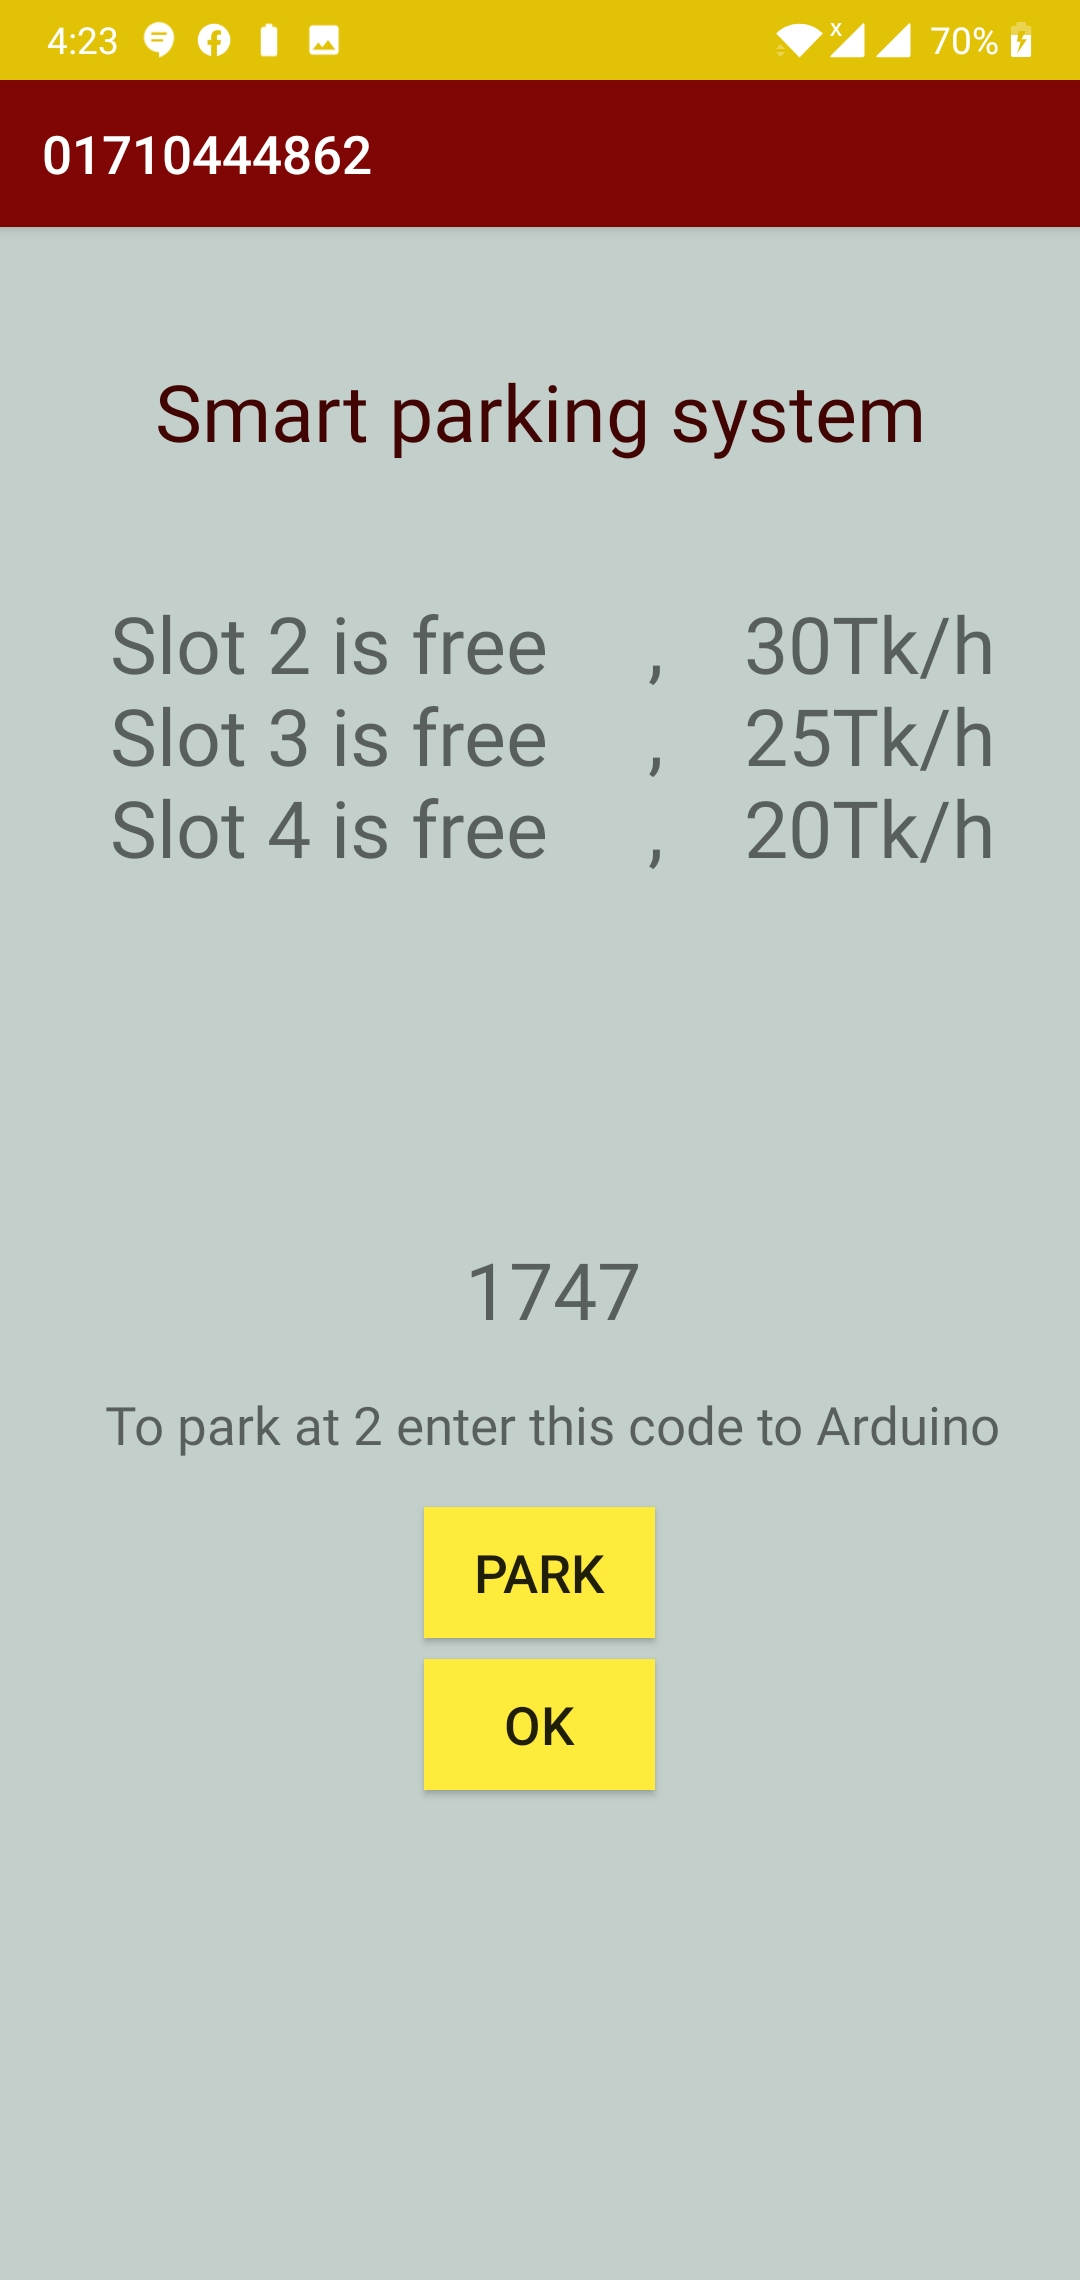
\includegraphics[width = 0.4\textwidth]{figures/password_generation_m.jpg}
\label{password_generation}}
\hspace{1cm}
\subfloat[Slot Number inputting]{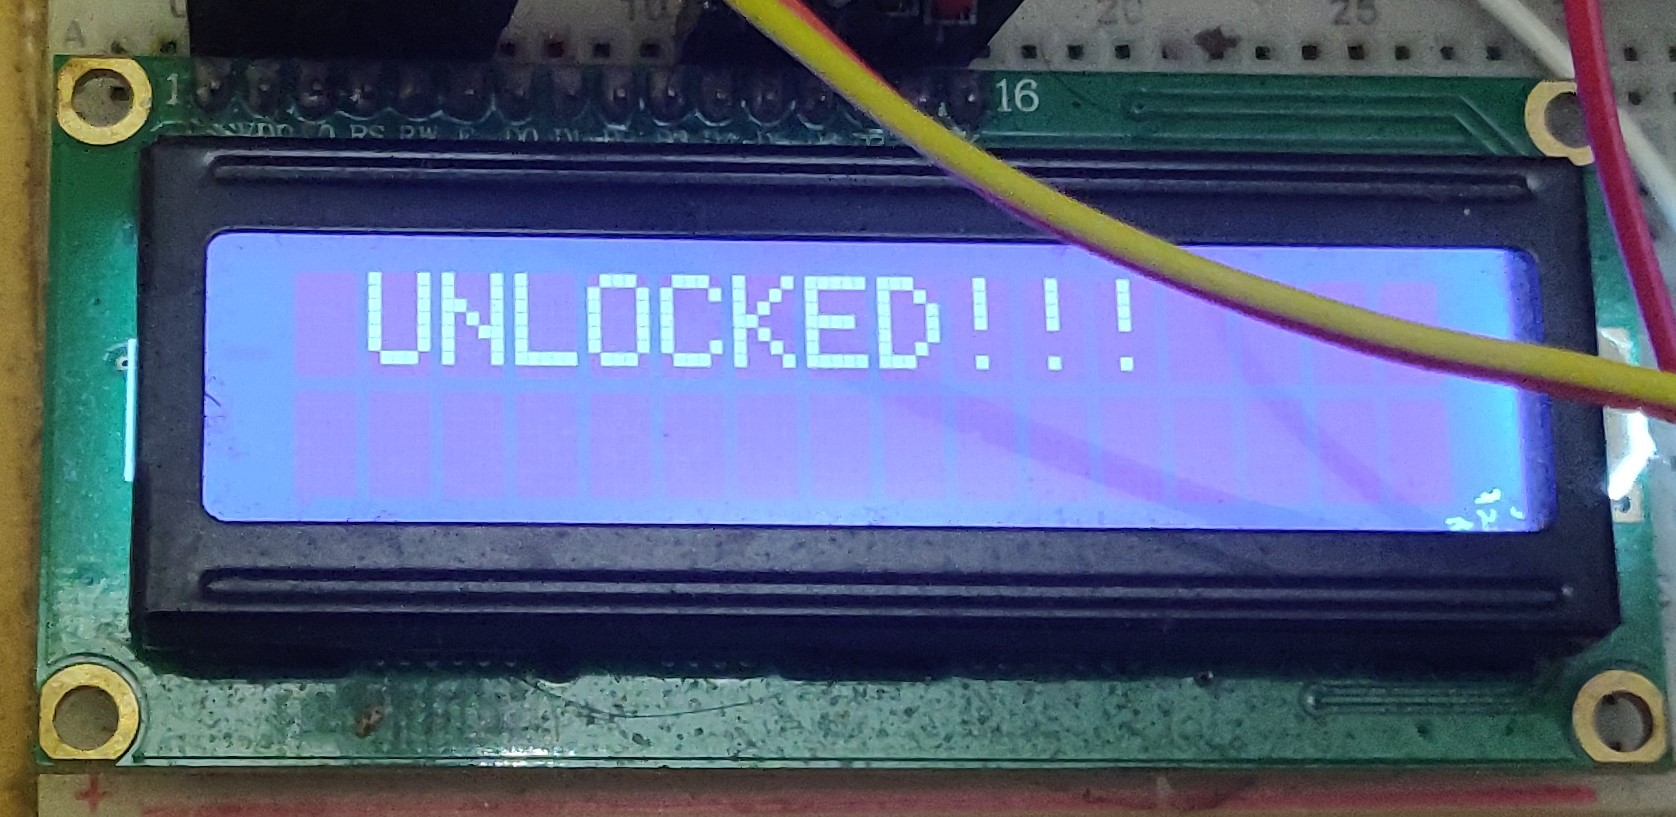
\includegraphics[width = 0.4\textwidth]{figures/unlocked.jpg}
\label{unlocked}}
\vspace{1cm}
\subfloat[Time and Slot Updated at Server]{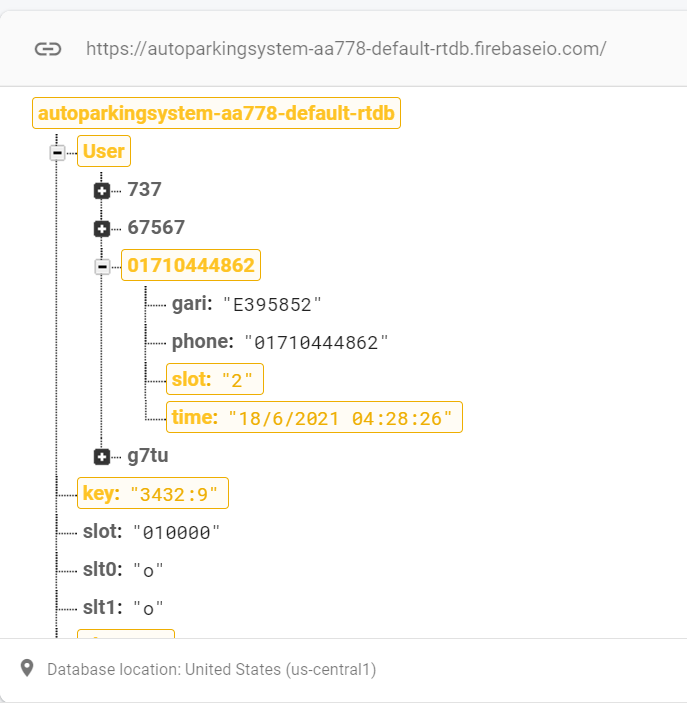
\includegraphics[width = 0.7\textwidth]{figures/time_updating1.png}
\label{Time_and_Slot_Updated_Server}}
\hspace{1cm}
\caption{Slot Allocation}
\end{figure}

\subsection{Car Security}
We developed car security feature which monitors parked car until unpark. To unpark only that application is to be used in which information is saved. Without logged in unparking can not be possible. At starting application checks that car is parked or not if car is parked, automatically unparked button activates \ref{parked_at_slo2}. During unparked at database it in his profile it is written that car parking time is not '0'. In this parked state if car is displaced without requesting unpark and paying for application, the system considers that someone is trying to steal the car. Also without requesting for unpark and completing payment procedure from application the gates can not be opened. The slot at which car was  parked is denoted by '1' and if not parked it denoted by '0'. If any slot status change from '1' to '0', arduino checks that the payment is completed or not. If not then it tells server that sealing is going on and an early alarm starts with buzzer. And using GSM module it sends warning message to the respective person \ref{warningsms}. At the same time android gets stealing information from server and makes an anti theft alarm even phone is in locked state \ref{alarmm}. This procedure is Shown in flow chart \ref{alarm_flow}.

\begin{figure}[H]
\centering
\subfloat[Alarm Making Flow Chart]{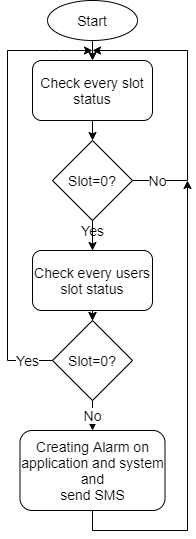
\includegraphics[width = 0.4\textwidth]{figures/Alarm_flow.png}
\label{alarm_flow}}
\hspace{1cm}
\subfloat[Parked at Slot 2]{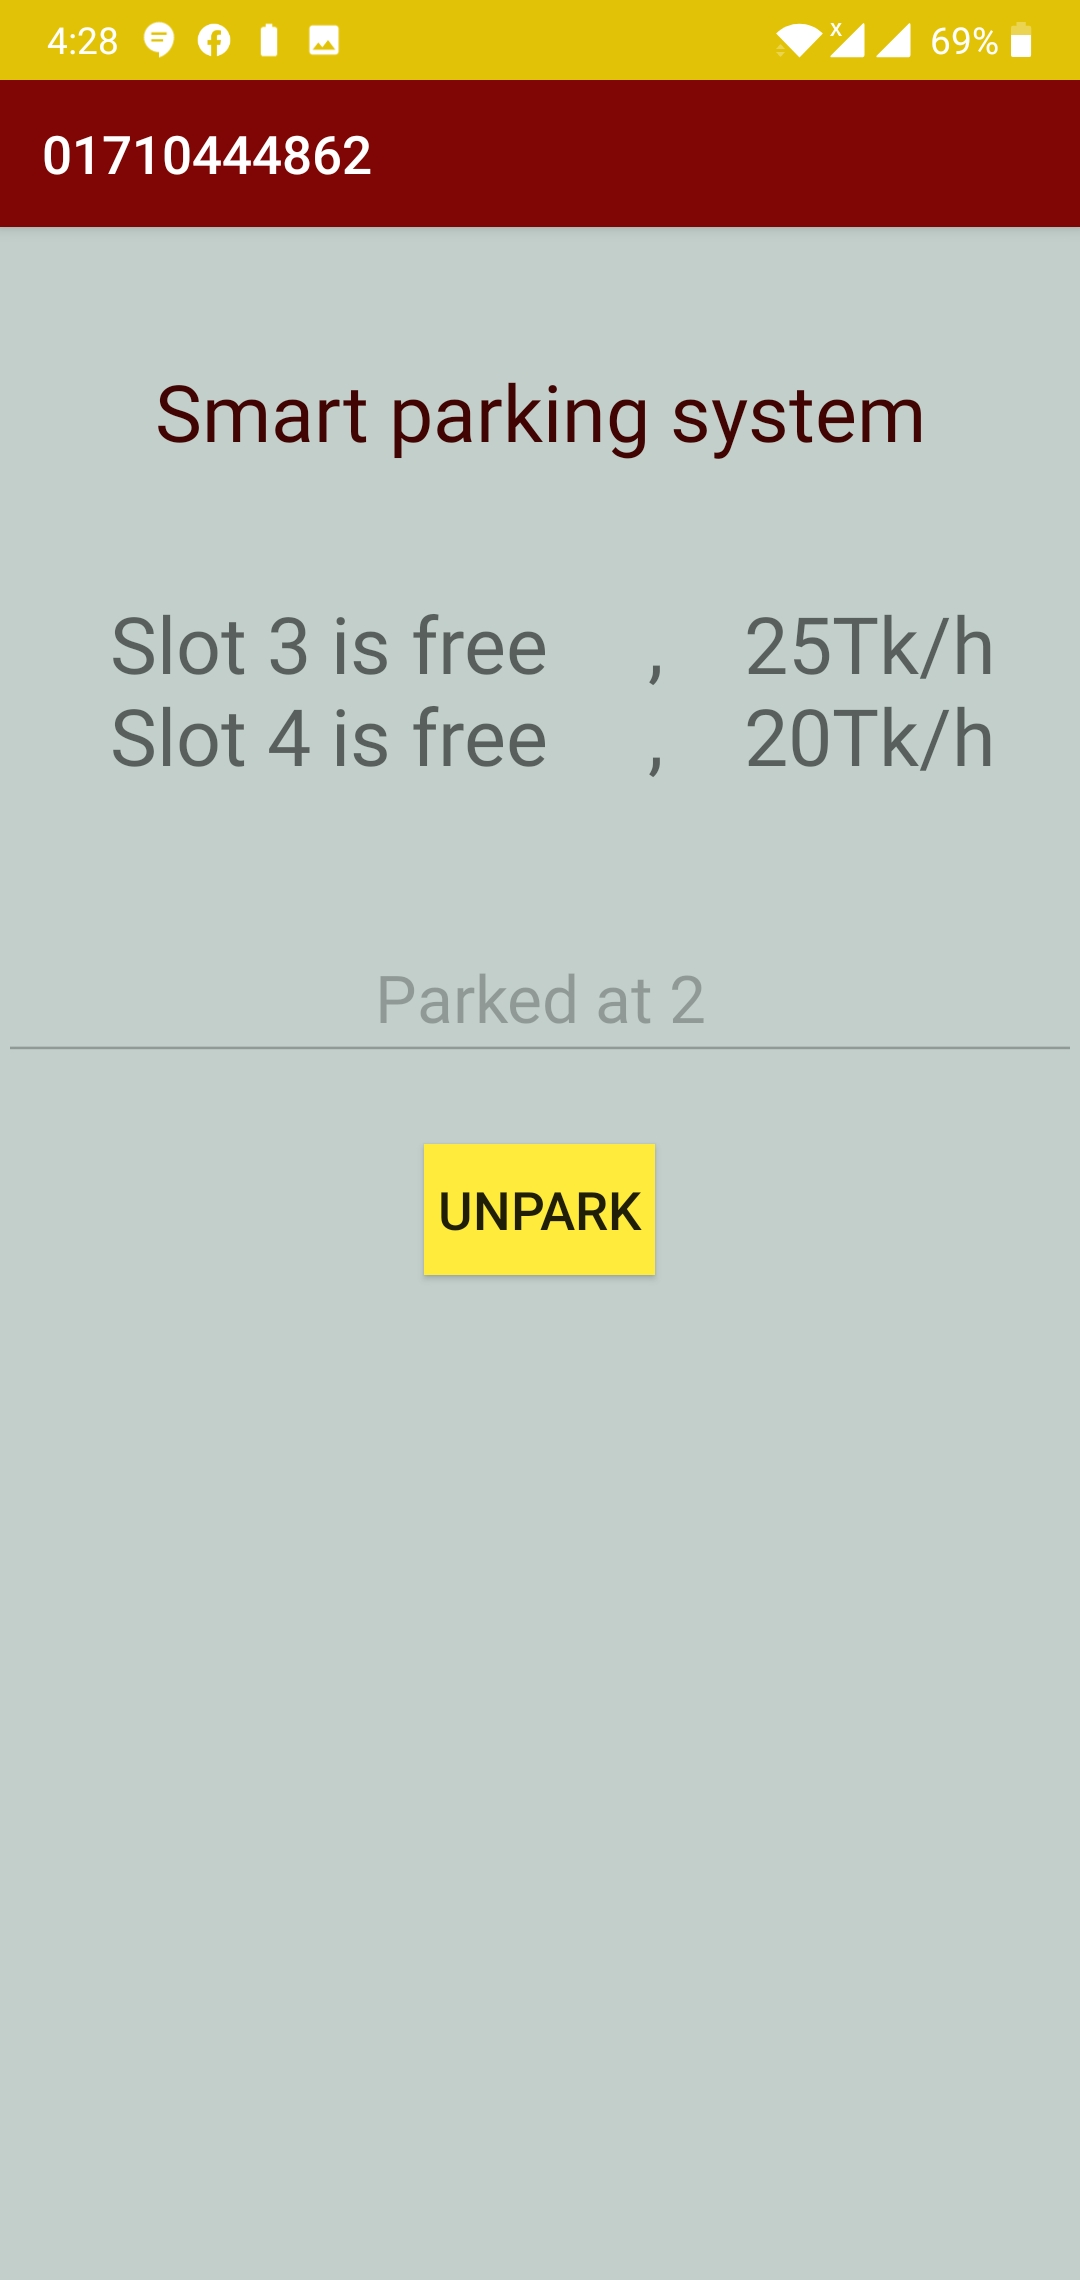
\includegraphics[width = 0.4\textwidth]{figures/parked2_m.jpg}
\label{parked_at_slo2}}
% \caption{Activated Unpark Button and Seurity Alarm}
\end{figure}

\begin{figure}[H]
\centering
\subfloat[Incoming Warning Message]{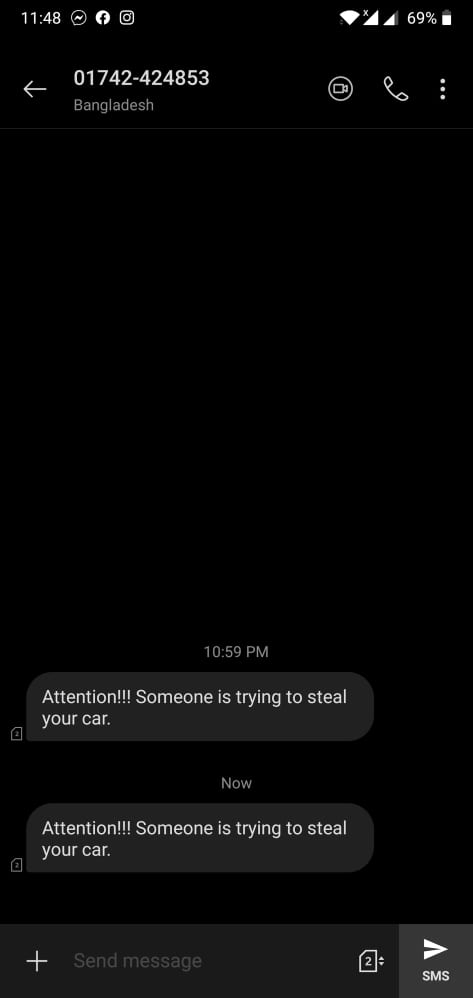
\includegraphics[width = 0.4\textwidth]{figures/incomming_sms.jpg}
\label{warningsms}}
\hspace{1cm}
\subfloat[Anti Theft Alarm on Application]{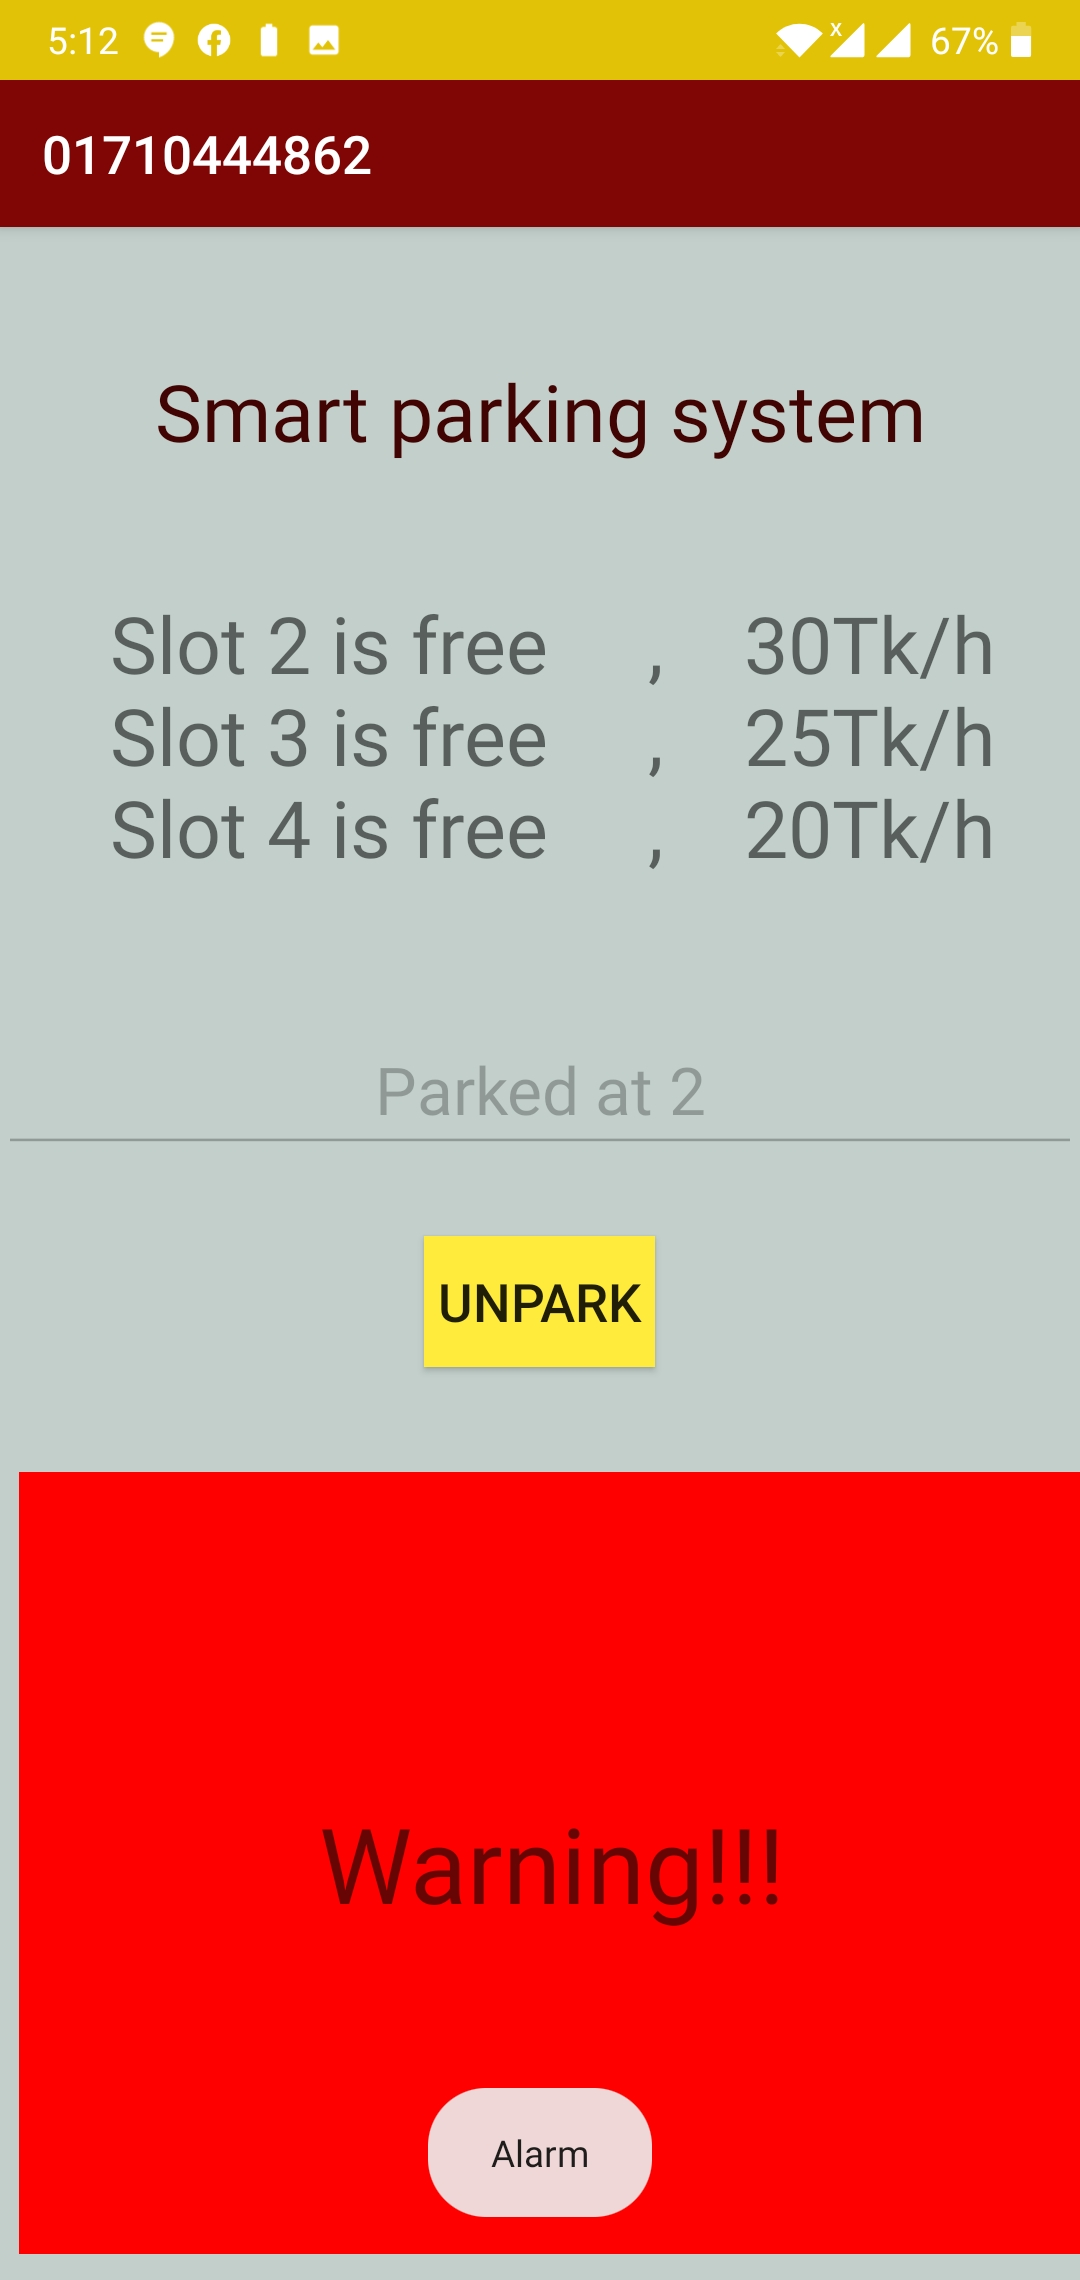
\includegraphics[width = 0.4\textwidth]{figures/Alarm.jpg}
\label{alarmm}}
\caption{Activated Unpark Button and Seurity Alarm}
\end{figure}

\subsection{Pricing and Payment}
We fixed different fare for different slot as different slot has different distance from entry gate\ref{price_slots}. Emergency slot has the highest price, and as the distance increases from gate the slot fare is decreases. We set pricing by hour. Emergency slot has 40 taka fare, and 2, 3, 4 has 30, 25, 20 taka accordingly. We added E-walet mobile banking Bkash and Nagod for finishing payment electronically from application automatically \ref{mobile_banking}. When requsts for unpark, application reads time and slot number from database, calculates the time in hour and multiplying fare with time it calculates the bill. Then application checks users account balance \ref{Bal_before}, if there is sufficient amount of money it deducts money automatically and opens gate for leaving the car. We can see the balance before unparking \ref{Bal_before}, deducted calculated money \ref{money_deduct} and new balance after deducting money \ref{Bal_after}. After successfully unparked information is updated on firebase realtime cloud server \ref{information_updates}.

\begin{figure}[H]
\centering
\subfloat[Price of Different slots]{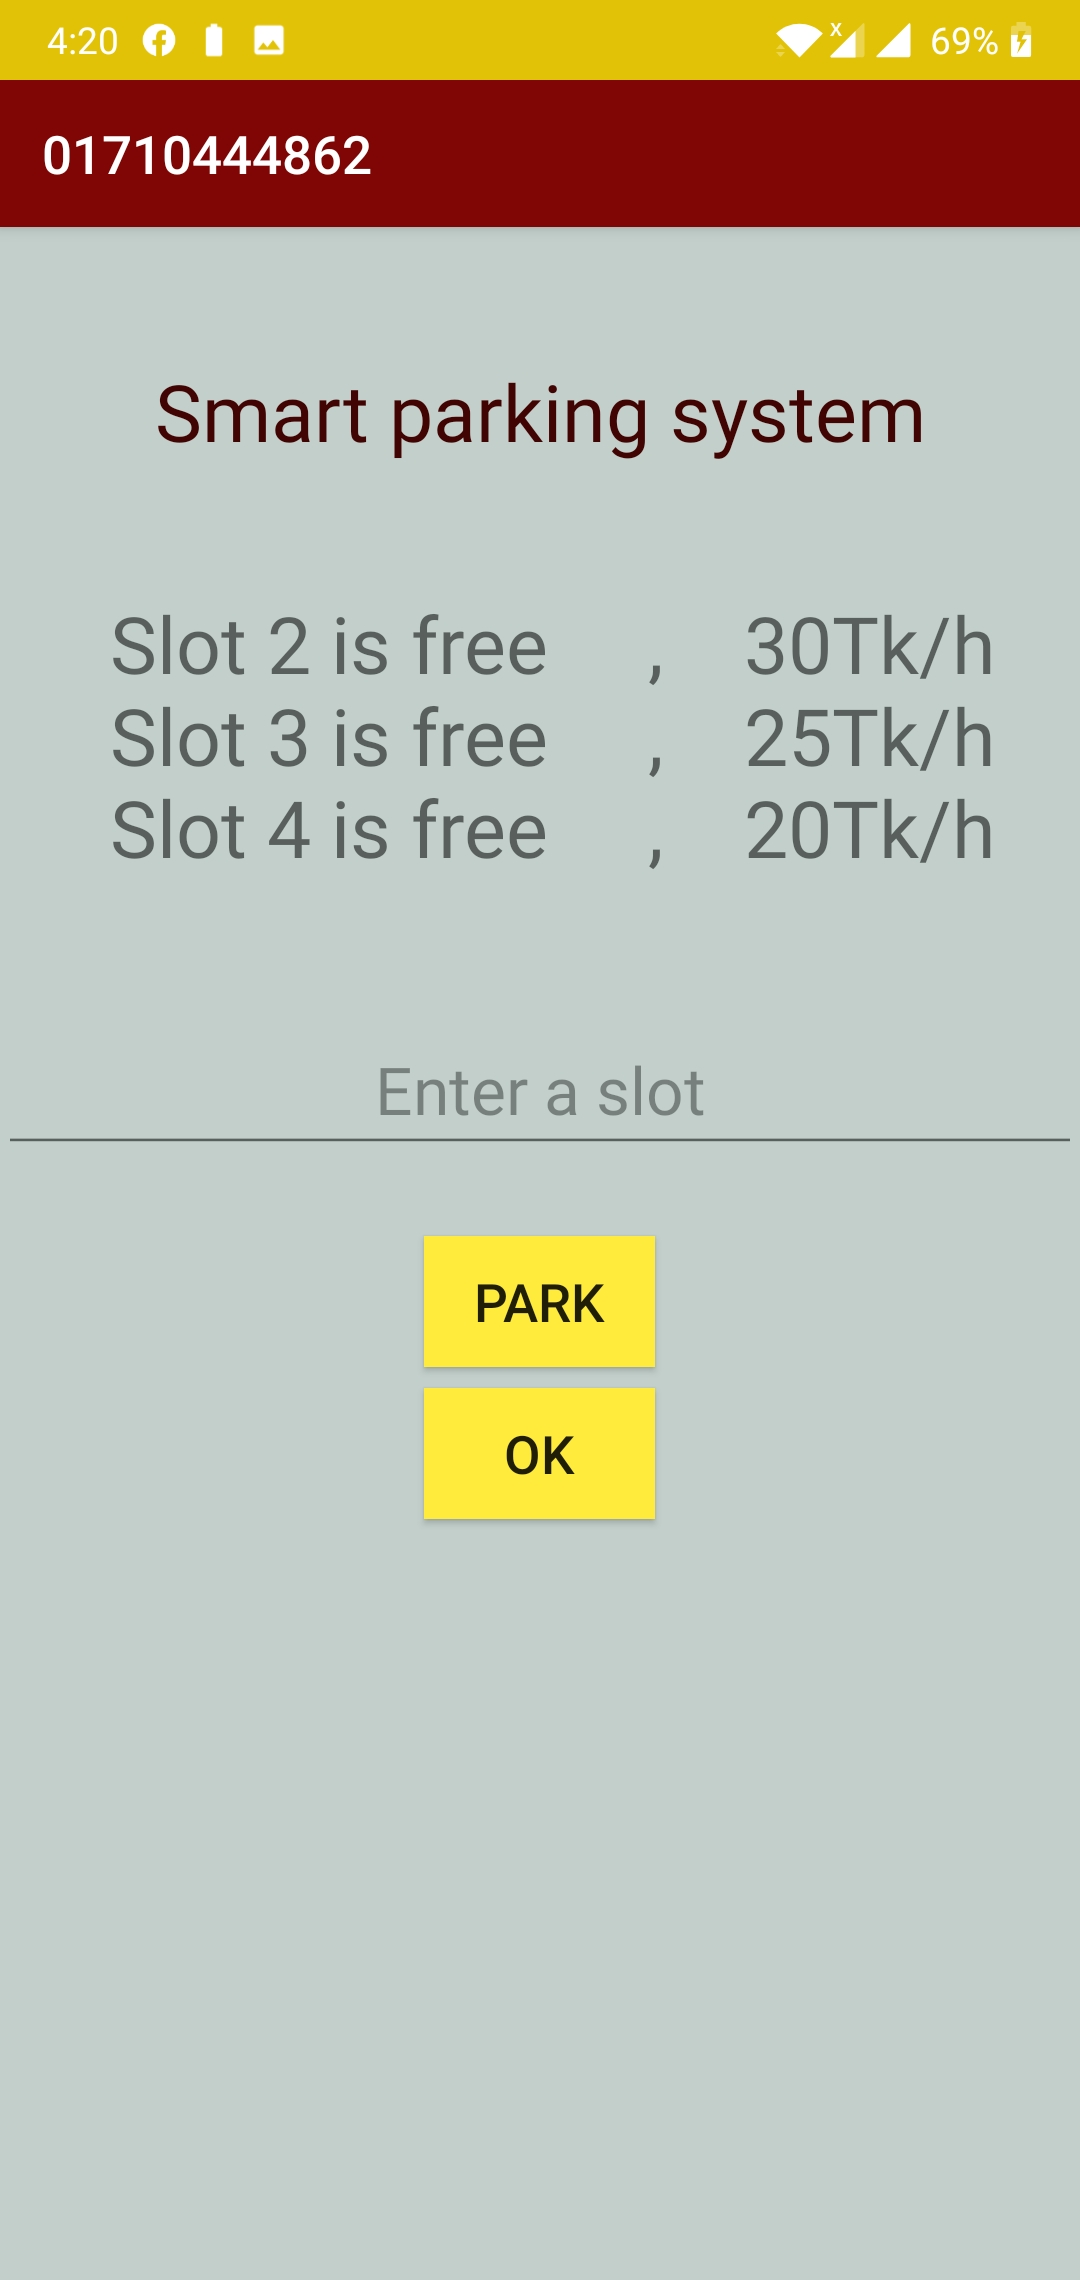
\includegraphics[width = 0.4\textwidth]{figures/non_slot_m.jpg}
\label{price_slots}} 
\hspace{1cm}
\subfloat[Mobile Banking]{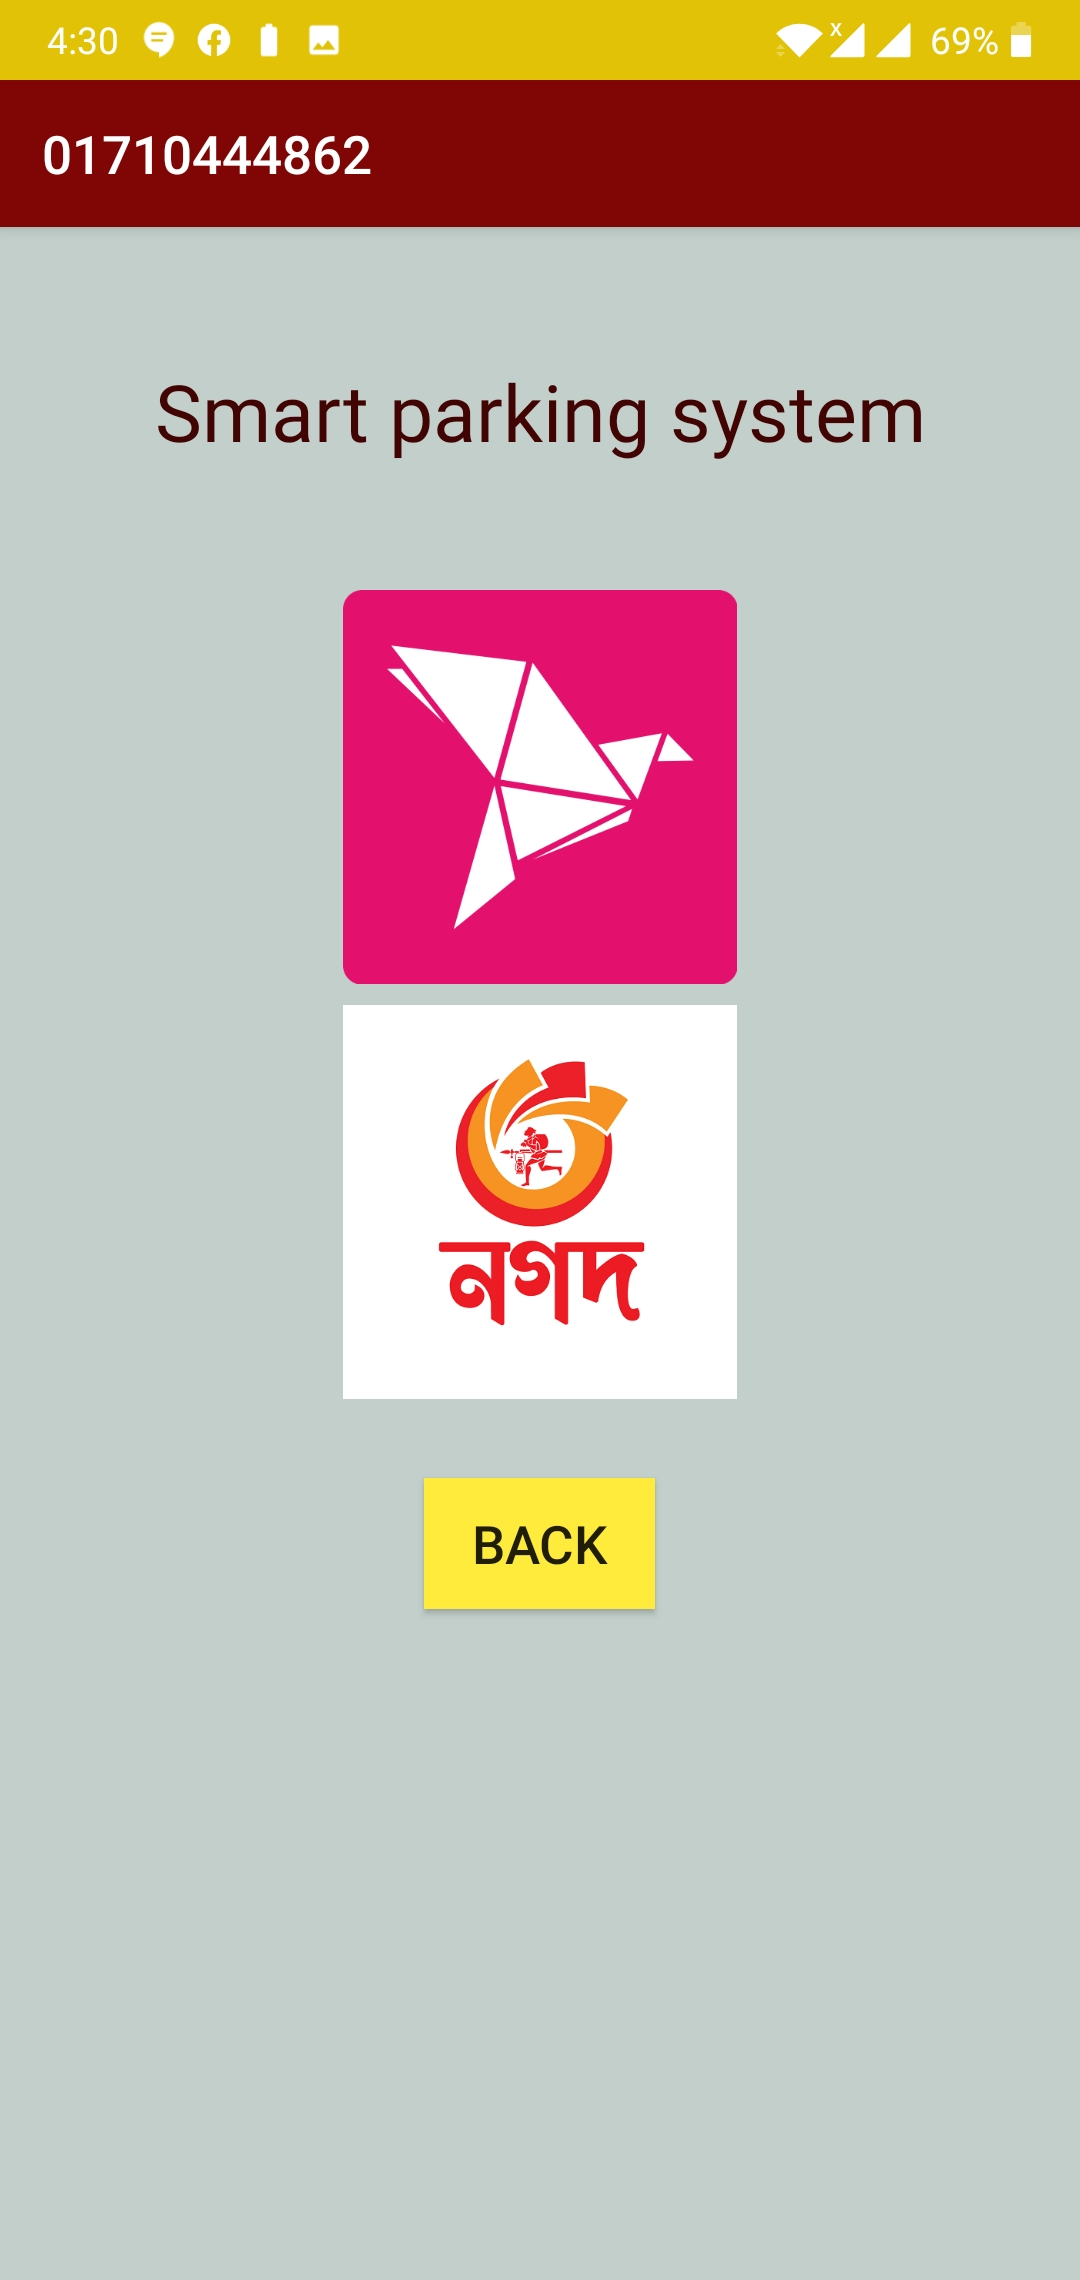
\includegraphics[width = 0.4\textwidth]{figures/bkash_nogod.jpg}
\label{mobile_banking}}
% \caption{Login Interface and Profile Creation}
\end{figure}

\begin{figure}[H]
\centering
\subfloat[Balance Before Unpark]{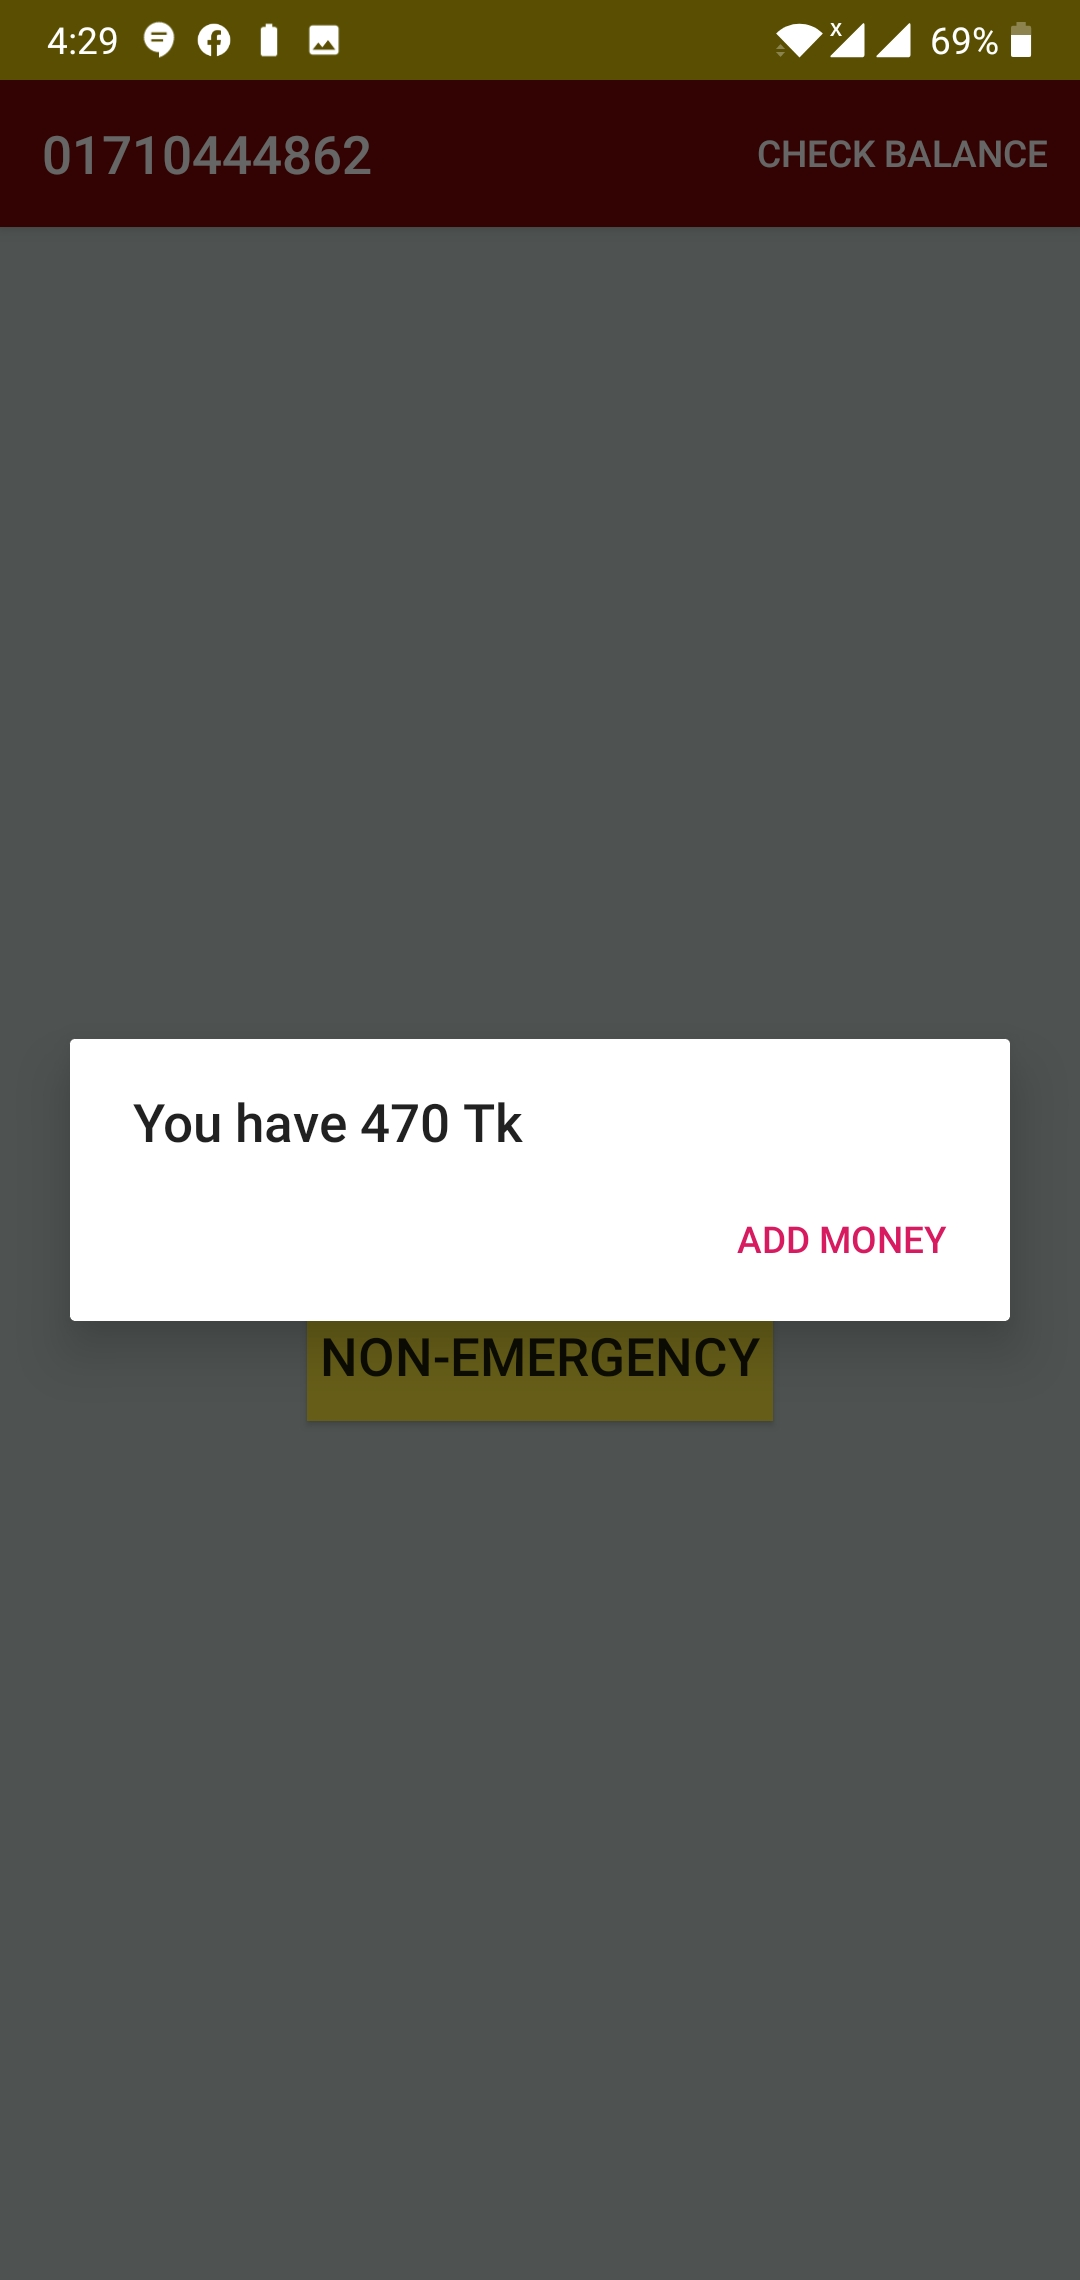
\includegraphics[width = 0.35\textwidth]{figures/balance_check_m.jpg}
\label{Bal_before}} 
\hspace{1cm}
\subfloat[Money deducted]{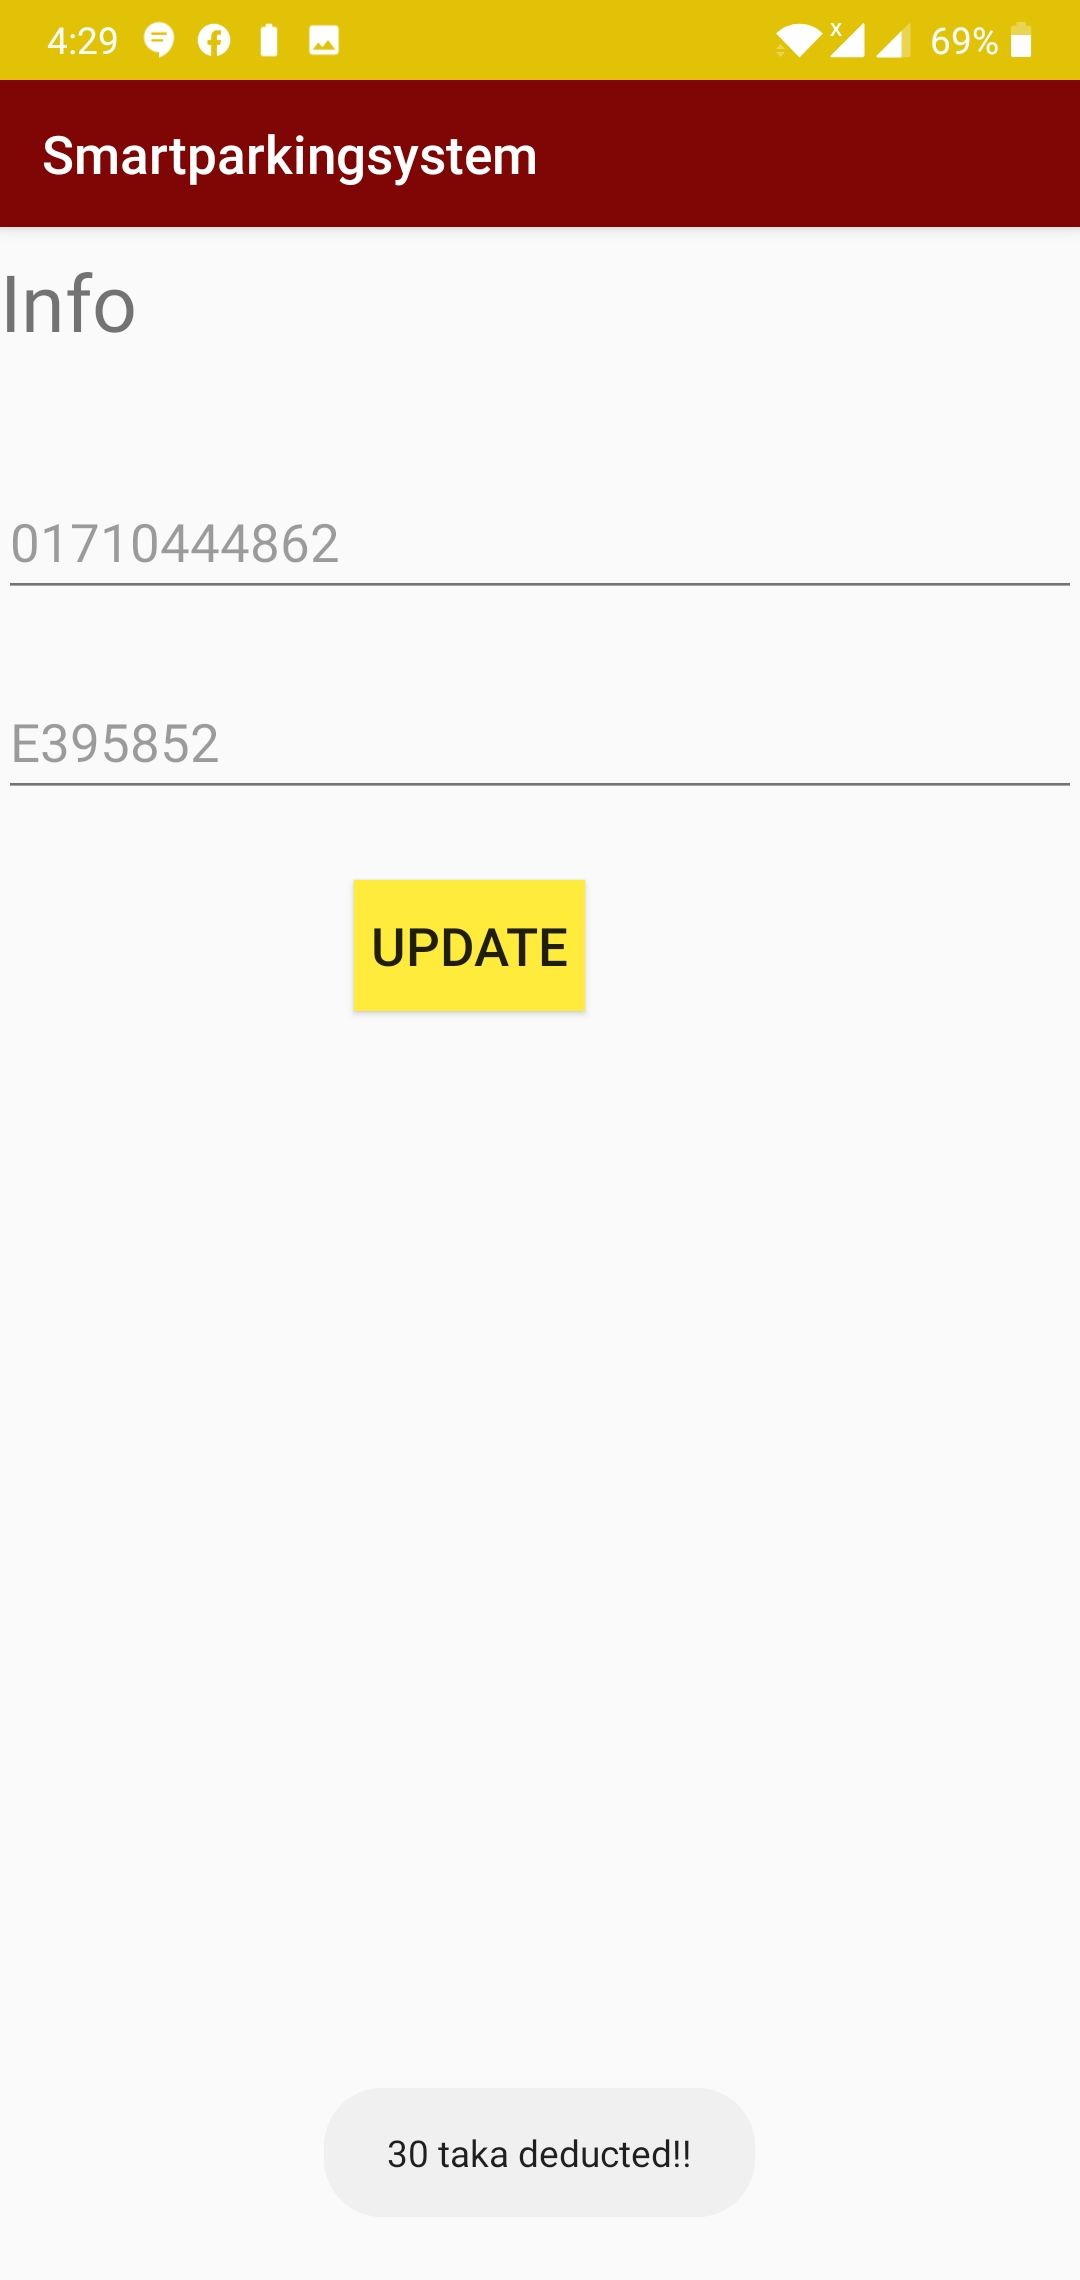
\includegraphics[width = 0.35\textwidth]{figures/taka_deducted.jpg}
\label{money_deduct}}
% \caption{Login Interface and Profile Creation}
\end{figure}

\begin{figure}[H]
\centering
\subfloat[Balance After Unpark]{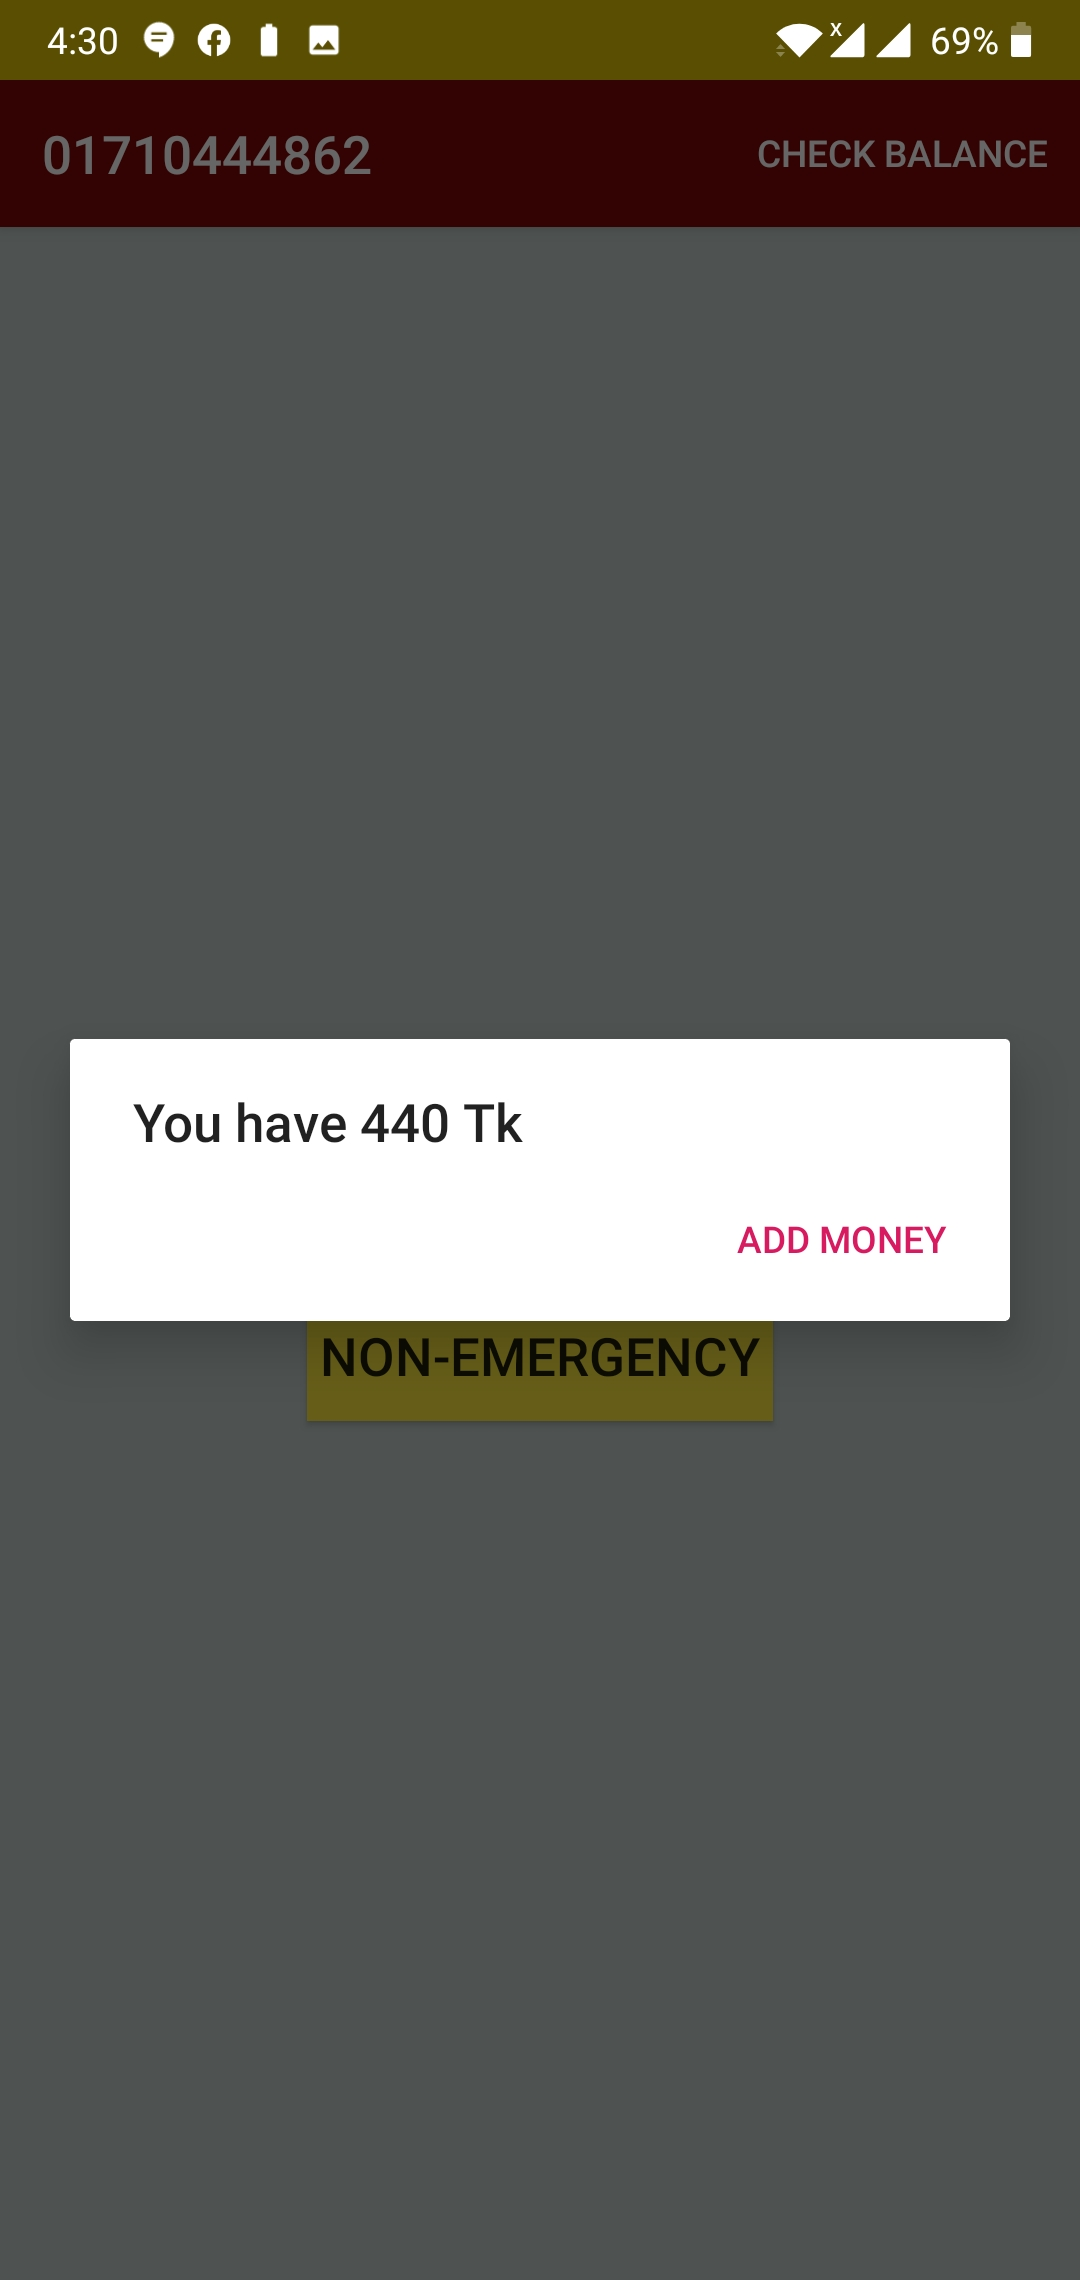
\includegraphics[width = 0.35\textwidth]{figures/new_balance_m.jpg}
\label{Bal_after}} 
\hspace{1cm}
\subfloat[Information updating]{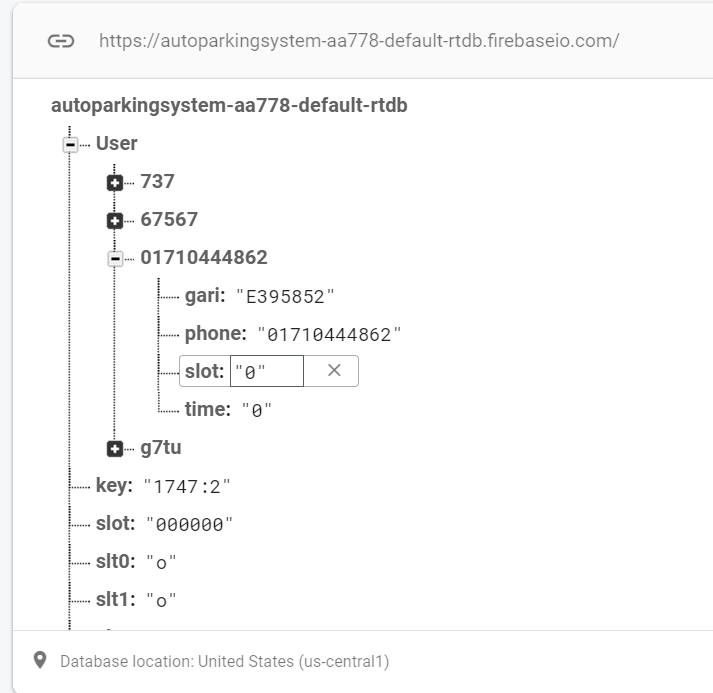
\includegraphics[width = 0.35\textwidth]{figures/time_updating2.png}
\label{information_updates}}
\caption{Pricing and payment Process}
\end{figure}

\subsection{Suggest Another Slot}
This system is designed focusing on real life car parking spot. Thus if the nearest parking spot is full then application will suggest the next nearest spot. 

\begin{figure}[H]
\centering
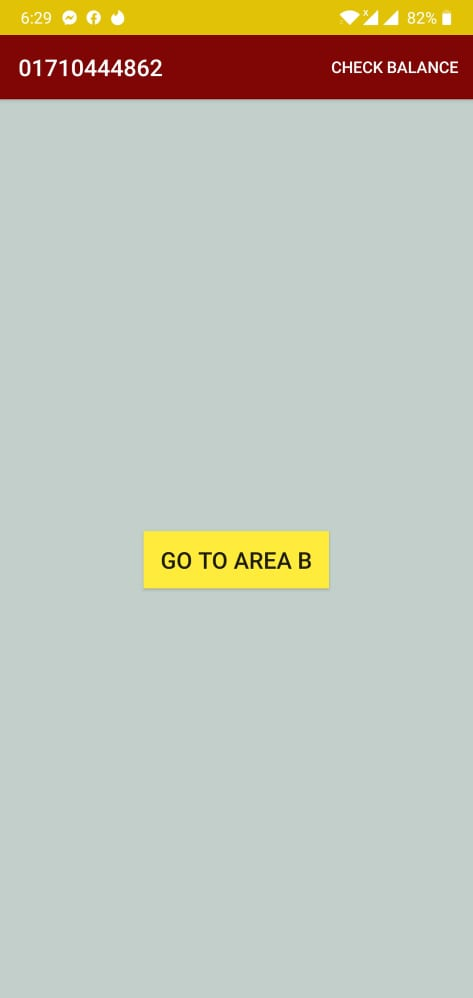
\includegraphics[width=0.5\textwidth]{figures/go2areab.jpg}
\caption{Suggest to Go to Next Nearest Spot}
\label{goto}
\end{figure}
Figure \ref{goto} represents that application suggests to go to the next nearest spot B as the nearest parking spot A has not any free slot.

\section{Conclusion}
In this section we discussed on the working principle, methodology, how hardware and software, database server collaborate with each other, how logics are implemented and features like reading slot status, requesting for slot, pin verification, emergency and non emergency slot's working mechanism, monitoring for security, automatically opening of gates, pricing and mobile payment are vastly described with figures, diagrams and flow charts here. In the following chapter we will discuss on the result and performance of our system. 
